%DIF 1a1
%DIF LATEXDIFF DIFFERENCE FILE
%DIF DEL /Users/duco/Documents/Thesis_Vorig/thesisDW.tex   Fri Nov 29 08:40:10 2013
%DIF ADD thesisDW.tex                                      Sun Dec  8 19:11:53 2013
\documentclass[titlepage,openright,11pt]{report} %titlepage,  ,twoside%&thesisdw %DIF > 
%DIF -------

%DIF 2d3
%DIF < \documentclass[titlepage,openright,11pt]{report} %titlepage,,twoside,
%DIF -------

%DIF 4d4
%DIF < %--------------------PREAMBLE----------------------------------------
%DIF -------

%DIF 6a5
%--------------------PREAMBLE---------------------------------------- %DIF > 
%DIF -------
\usepackage{setspace}% benodigd voor spacing commando
\usepackage[nottoc]{tocbibind}
\usepackage{titlesec}
%\usepackage{eucal}
\usepackage[usenames,dvipsnames]{xcolor} %
\usepackage{datetime} % gebruikt voor \pdfdate om juiste datum weergave te krijgen
\usepackage{fancyhdr}
\usepackage{graphicx}%[pdftex]
\usepackage[utf8]{inputenc} %f ̧r Windows %direct gebruik van accenten
\input{ix-utf8enc.dfu}% dit is om u ̃ te laden
%\usepackage[T1]{fontenc}
\usepackage{eurosym,tfrupee,supertabular} %tfrupee om het rupee symbool te maken 
\usepackage[a4paper]{geometry}
\usepackage{rotating}
%\usepackage{parskip}
\usepackage[small,bf,up]{caption}%[2004/07/16]
\usepackage{tablefootnote}
\usepackage{amsthm}% package om te assisteren bij Working Proposistions
\usepackage{url} % om urls goed weer te geven in voetnoten
\usepackage[toc,page,title]{appendix}
\usepackage[multiple,flushmargin,stable]{footmisc}
\usepackage{datatool} %databases laden in latex
\usepackage{booktabs}% om mooie tabellen te maken
%\usepackage{hanging}% provides the \hangpara command
%\usepackage{enumitem}
\usepackage{enumerate}
\usepackage{float} %gebruikt om floatplacement te activeren
\usepackage{tabularx,ragged2e} %in samenwerking met tabularx
\newcolumntype{Y}{>{\RaggedRight\arraybackslash}X} % modified "X" column
\usepackage{multirow}%
\RequirePackage[l2tabu, orthodox]{nag}
\usepackage{fixltx2e}% moet enkele latex fouten corrigeren
\usepackage{tikz} % tekenen van plaatjes
\usepackage{xspace} %correcte 'spaties' achter en voor comments en punten/comma'
\usepackage[protrusion=true,expansion]{microtype} %spacing tussen letters enzo 
\usetikzlibrary{arrows,shapes,decorations.pathmorphing,backgrounds,fit,positioning,shapes.symbols,chains}
\usetikzlibrary{external}
\tikzexternalize[prefix=TikzFigures/]
\tikzexternalize
%\usepackage{illcmolthesis} %dit maakt de titel pagina

\doublespacing%

    \definecolor{gray75}{gray}{0.75}
    \DeclareGraphicsExtensions{.png, .jpg, .pdf}%
    \pdfcompresslevel=9
    \graphicspath{{./Figures/}}

%\DeclareUnicodeCharacter{0169}{\~u} % make the character known
%\DeclareUnicodeCharacter{226}{\^a}

%--------------Layout van A4 document-----------------
\geometry{a4paper,
  %includefoot,
 % margin=2.5cm,
  %hdivide={ ,19cm, }  
}

%------------------Footnotes--------------------------
%\renewcommand{\footnotemargin}{1em}% onderdeel van footnotemisc
% changes the above and sets the footnote mark just right of the left margin border.

%\newcommand{\fn}[1]{\footnote{\hangpara{3em}{1} #1}}
% makes a new footnote command \fn{} with a hanging indent of 3em (hanging indent starts after the first line)

%------------Biblatex Optie 1---------------------------

%%\usepackage[backend=biber,style=authoryear-luh-ipw,isbn=false,url=false]%{biblatex} ,style=historian ,citestyle=apa
\usepackage[
backend=biber,
citestyle=authoryear-icomp,
bibstyle=authortitle,
sorting=nyt,
bibencoding=utf8,
dashed=false,
maxcitenames=1,
isbn=false,
url=false,
babel=hyphen,
hyperref=true,
doi=false]
{biblatex}

\let\cite\textcite


\renewcommand*{\nameyeardelim}{\addcomma\space}
\renewcommand*{\postnotedelim}{\addcolon\space}
\DeclareFieldFormat{postnote}{#1}
\DeclareFieldFormat{multipostnote}{#1}

\usepackage{xpatch}
\xpretobibmacro{date+extrayear}{\addperiod\space}{}{}
\xapptobibmacro{date+extrayear}{\nopunct}{}{}


% Citation Hyperlinks (not just years), thanks to Audrey.
\makeatletter
\renewbibmacro*{cite}{% Based on cite bib macro from authoryear-comp.cbx
  \iffieldundef{shorthand}
    {\ifthenelse{\ifnameundef{labelname}\OR\iffieldundef{labelyear}}
       {\printtext[bibhyperref]{% Include labelname in hyperlink
          \DeclareFieldAlias{bibhyperref}{default}% Prevent nested hyperlinks
          \usebibmacro{cite:label}%
          \setunit{\addspace}%
          \usebibmacro{cite:labelyear+extrayear}}%
          \usebibmacro{cite:reinit}}
       {\iffieldequals{namehash}{\cbx@lasthash}
          {\ifthenelse{\iffieldequals{labelyear}{\cbx@lastyear}\AND
                       \(\value{multicitecount}=0\OR\iffieldundef{postnote}\)}
             {\setunit{\addcomma}%
              \usebibmacro{cite:extrayear}}
             {\setunit{\compcitedelim}%
              \usebibmacro{cite:labelyear+extrayear}%
              \savefield{labelyear}{\cbx@lastyear}}}
          {\printtext[bibhyperref]{% Include labelname in hyperlink
             \DeclareFieldAlias{bibhyperref}{default}% Prevent nested hyperlinks
             \printnames{labelname}%
             \setunit{\nameyeardelim}%
             \usebibmacro{cite:labelyear+extrayear}}%
             \savefield{namehash}{\cbx@lasthash}%
             \savefield{labelyear}{\cbx@lastyear}}}}
    {\usebibmacro{cite:shorthand}%
     \usebibmacro{cite:reinit}}%
  \setunit{\multicitedelim}}
%--------Biblatex-------------------------------------

%\DeclareNameAlias{sortname}{first-last}

%\DeclareCiteCommand{\cite}[\mkbibbrackets]
 % {\usebibmacro{prenote}}
 % {\usebibmacro{citeindex}%
  % \usebibmacro{cite}}
%  {\multicitedelim}
%  {\usebibmacro{postnote}}

%\DeclareCiteCommand*{\cite}[\mkbibbrackets]
%  {\usebibmacro{prenote}}
 % {\usebibmacro{citeindex}%
%   \usebibmacro{citeyear}}
%  {\multicitedelim}
 % {\usebibmacro{postnote}}


%\newcounter{mymaxcitenames}
%\AtBeginDocument{%
 % \setcounter{mymaxcitenames}{\value{maxnames}}%
%}

%\renewbibmacro*{begentry}{%
 % \printtext[brackets]{%
  %  \begingroup%
 %   \defcounter{maxnames}{\value{mymaxcitenames}}%
  %  \printnames{labelname}%
 %   \setunit{\nameyeardelim}%
 %   \usebibmacro{cite:labelyear+extrayear}%
 %   \endgroup%
  %  }%
%  \quad% or \addspace
%}

%--------END Biblatex-------------------------------------



%------------Biblatex Optie 2---------------------------

\usepackage[
        natbib=true,
        citestyle=authoryear-comp,
        bibstyle=authoryear,
        hyperref=false,
        backend=biber,
        %bibencoding=auto,
        maxbibnames=99,
        uniquename=false,
        maxcitenames=1,
        dashed=false,
        url=false,
        doi=false,
        isbn=false,
        eprint=false
                    ]{biblatex}
 
\renewcommand{\cite}{\textcite} 

% remove "in:" from articles. Thanks to Herbert.
\renewbibmacro{in:}{%
  \ifentrytype{article}{}{%
  \printtext{\bibstring{in}\intitlepunct}}}

% increase vertical space between bibliography items.
\setlength\bibitemsep{0.5ex}
\setlength\bibnamesep{1.2ex}

% makes volume of journal bold and adds colon
\DeclareFieldFormat[article]{volume}{\textbf{#1}\addcolon\space}


%\renewcommand*{\textcitedelim}{\addcomma\space}% if you want another delimiter

%\newcommand*{\mywrapper}[1]{%
%    \ifthenelse{\value{textcitetotal}>1}
%    {\mkbibbrackets{#1}}
%    {#1}}
%
%\makeatletter
%\DeclareMultiCiteCommand{\cbx@textcites}[\mywrapper]{\cbx@textcite}{} 
%
%\DeclareCiteCommand{\cbx@textcite}[\mywrapper]
%  {\usebibmacro{cite:init}}
%  {\usebibmacro{citeindex}%
%   \usebibmacro{textcite}}
%  {}
%  {\usebibmacro{textcite:postnote}}
%
%\makeatother


% Dit is de juiste definitie voor het gebruik van de bibs
%----------------------------CSQuotes na Biblatex
\usepackage[babel]{csquotes}%
\usepackage[english]{babel}%
%------------------ FONT ----------------------------------------

 \usepackage{pifont}%gebruik van checkmarkt
 \usepackage{charter}%
% ALTERNATIVE
%\usepackage{lmodern}
%\usepackage{fouriernc}
%\usepackage{MinionPro}
%\usepackage[urw-garamond]{mathdesign}
%\usepackage[math]{iwona}
%\usepackage[default]{lato}
%\usepackage{venturis2}
%\usepackage[sf]{quattrocento}
%\usepackage{libertine}



%--------Hyperref zo laat mogelijk------------------------

\usepackage[   pdftex, 
               %  plainpages = false, 
               %  pdfpagelabels, 
                % pdfpagelayout = OneColumn, 
               %   display single page, advancing flips the page - Sasa Tomic
                % bookmarks,
               %  bookmarksopen = true,
                % bookmarksnumbered = true,
               %  breaklinks = true,
                % linktocpage,
                 colorlinks = false,
                % linkcolor = black,
                % urlcolor  = black,
                % citecolor = black,
                % anchorcolor = black,
                 hyperindex = true,
               %  pageanchor = false,
                % hyperfigures
                 ]{hyperref}% als laatste laden om conflicten te voorkomen 
%----------einde titel opmaak-------------------
\floatplacement{table}{htbp} 
\floatplacement{figure}{htbp}
\setlength{\columnseprule}{\headrulewidth}
\setcounter{tocdepth}{2}

%------------------ END FONT ------------------

\linespread{1.5} %\setlength{\parskip}{\baselineskip}
\setlength{\headheight}{43,3pt}
\setlength{\voffset}{0pt}

\fancypagestyle{plain}{\fancyhf{}\fancyfoot[R]{\thepage}
\renewcommand{\headrulewidth}{0.4pt}
\renewcommand{\footrulewidth}{0.4pt}
}

\pagestyle{fancy}
\fancyhf{}     % clear header & footer
\fancyhead[C]{\small\sffamily\nouppercase{\leftmark}}
%\fancyhead[L]{\includegraphics[width=.19\textwidth]{uva_logo_eng.eps}} %links logo
\fancyhead[R]{
\includegraphics[width=.19\textwidth]{uva_ENG.eps}}  %rechts logo
%\fancyfoot[L]{\thepage}
\fancyfoot[R]{\thepage}
\renewcommand{\headrulewidth}{0.4pt}
\renewcommand{\footrulewidth}{0.4pt}

\renewcommand{\captionfont}{\small\textit}

\renewcommand{\headrule}{{\color{gray}%
\hrule width\headwidth%
 height\headrulewidth \vskip-\headrulewidth}
 }

\renewcommand{\footrule}{{\color{gray}% 
  \vskip-\footruleskip\vskip-\footrulewidth%
\hrule width\headwidth height\footrulewidth\vskip\footruleskip}
}
\renewcommand{\chaptermark}[1]{\markboth{\textbf{\thechapter\ #1}}{}}
\renewcommand{\sectionmark}[1]{\markright{\thesection\ #1}{}}
\fancyheadoffset{0cm} % zorgt er voor dat de head en foot lijnen even breed zijn als de textbreedte


%%%%% by default first HYPERREF than Glossaries packgages
\usepackage[acronym,toc,xindy,nomain]{glossaries}% 
\glsdisablehyper%
\makeglossaries%
%____________THEOREM___________

\makeatletter

\newenvironment{subtheorem}[1]{%
  \def\subtheoremcounter{#1}%
  \refstepcounter{#1}%
  \protected@edef\theparentnumber{\csname the#1\endcsname}%
  \setcounter{parentnumber}{\value{#1}}%
  \setcounter{#1}{0}%
  \expandafter\def\csname the#1\endcsname{\theparentnumber.\Alph{#1}}%
  \ignorespaces
}{%
  \setcounter{\subtheoremcounter}{\value{parentnumber}}%
  \ignorespacesafterend
}
\makeatother
\newcounter{parentnumber}


%%%%%%%%%% stukje code voor oplopend versie nummer%%%%%%%%%%%%%

\newcounter{run}
\usepackage{catchfile}
\IfFileExists{\jobname.runs}{%
  \begingroup
    \CatchFileEdef\tmp{\jobname.runs}{\endlinechar=-1\relax}%
    \setcounter{run}{\tmp}%
  \endgroup
}{}
\stepcounter{run}

\usepackage{atveryend}
\usepackage{newfile}
\AtVeryEndDocument{%
  \newoutputstream{runs}%
  \openoutputfile{\jobname.runs}{runs}%
  \addtostream{runs}{\number\value{run}}%
  \closeoutputstream{runs}%
}


%%%%%%%%%%%% aanvulling voor Latex Diff  %%%%%%%%%%%%%%
%\providecommand{\DIFadd}[1]{{\protect\color{blue}#1}} %%%% Dit staat in thesisdw document
%\providecommand{\DIFdel}[1]{{\protect\color{red}#1}  %%%% Dit staat in thesisdw document
%\providecommand{\DIFadd}[1]{{\protect\color{blue}#1}} %DIF PREAMBLE  %%%% Dit staat in thesisdw document
%\providecommand{\DIFdel}[1]{{\protect\color{red}\protect\scriptsize{#1}}}  %%%% Dit staat in thesisdw document
%DIF 7c7
%DIF < %\endofdump %&thesisdw
%DIF -------
%\endofdump  %DIF > 
%DIF -------
%---------Bibliography--------------------------------
\bibliography{Biblio/Thesis_bib,Biblio/websites,Biblio/Bibliography_papers,Biblio/Westney}% 
%DIF 10-12c10-11
%DIF < % turn of those nasty overfull and underfull hboxes
%DIF < \hbadness=10000%
%DIF < \vbadness=10000%
%DIF -------
 %turn of those nasty overfull and underfull hboxes %DIF > 
\hbadness=10000 \vbadness=10000% %DIF > 
%DIF -------
%\hfuzz=40pt

%-------------Titel informatie----------------------
%DIF 16d15
%DIF < %Wordt in make title genereerd
%DIF -------
%\begin{titlepage}
\title{Effects of Institutions on International Business}
\subtitle{Does the WTO effect firms in advanced and emerging economies differently?}   

   \hypersetup{%    
    pdfinfo={%
    Title={Effect of Institutions on IB},
               %/Creator (TeX)
    Producer={pdfTeX},
    Author={Duco Wiertsema},
    CreationDate={D:20131015161832}, %format D:YYYYMMDDhhmmss
    ModDate={D:\pdfdate},
    Subject={Institutions and International Business},
    Keywords={Msc, Thesis, Duco Wiertsema},
              }
                 }
    \pdfcatalog { /PageMode (/UseOutlines)
                  /OpenAction (fitbh)  }

\author{\huge \href{mailto:duco@wiertsema.net}{Duco Wiertsema}\\ \large{6369332}}
\supervisor{Johan Lindeque}
\supervisor{Erik Driksen, Msc}
\date{\today}
 \FreeText{\small{Version: V0.9\therun}}


%---------BEGIN DOCUMENT----------------------------

\DTLloaddb[keys={Date,USD,JPY,BGN,CZK,DKK,GBP,HUF,LTL,LVL,PLN,RON, SEK,CHF,NOK,HRK,RUB,TRY,AUD,BRL,CAD,CNY,HKD,IDR,INR,KRW,MXN,MYR,NZD,PHP,SGD,THB,ZAR,ILS}]{Rates}{Appendices/eurofxref.csv}% Load database
%DIF 21d19
%DIF < 
%DIF -------
\DTLgetvalue{\ExRupee}{Rates}{1}{25}% \ExRupee is de exchange rate van de rupee
\DTLgetvalue{\ExDollar}{Rates}{1}{2}% \ExDollar is de exchange rate van de Dollar
\DTLgetvalue{\ExPound}{Rates}{1}{7}% \ExDollar is de exchange rate van de Pound
%DIF 25-27c22
%DIF < 
%DIF < 
%DIF < 
%DIF -------
% %DIF > 
%DIF -------
%\includeonly{Intro/Introduction}
\includeonly{LitReview/Literature_Review}
\includeonly{Metho/Methodology}
\includeonly{Resultaten/resultaten}
\includeonly{Discussion/Discussion}
%\includeonly{Conslusions/Conclusions}
\includeonly{Appendices/Appendix}
\makeglossaries %DIF > 
%DIF PREAMBLE EXTENSION ADDED BY LATEXDIFF
%DIF CTRADITIONAL PREAMBLE %DIF PREAMBLE
\RequirePackage{color}\definecolor{RED}{rgb}{1,0,0}\definecolor{BLUE}{rgb}{0,0,1} %DIF PREAMBLE
\RequirePackage[stable]{footmisc} %DIF PREAMBLE
\providecommand{\DIFadd}[1]{{\protect\color{blue} \sf #1}} %DIF PREAMBLE
\providecommand{\DIFdel}[1]{{\protect\color{red} [..\footnote{removed: #1} ]}} %DIF PREAMBLE
%DIF SAFE PREAMBLE %DIF PREAMBLE
\providecommand{\DIFaddbegin}{} %DIF PREAMBLE
\providecommand{\DIFaddend}{} %DIF PREAMBLE
\providecommand{\DIFdelbegin}{} %DIF PREAMBLE
\providecommand{\DIFdelend}{} %DIF PREAMBLE
%DIF FLOATSAFE PREAMBLE %DIF PREAMBLE
\providecommand{\DIFaddFL}[1]{\DIFadd{#1}} %DIF PREAMBLE
\providecommand{\DIFdelFL}[1]{\DIFdel{#1}} %DIF PREAMBLE
\providecommand{\DIFaddbeginFL}{} %DIF PREAMBLE
\providecommand{\DIFaddendFL}{} %DIF PREAMBLE
\providecommand{\DIFdelbeginFL}{} %DIF PREAMBLE
\providecommand{\DIFdelendFL}{} %DIF PREAMBLE
%DIF END PREAMBLE EXTENSION ADDED BY LATEXDIFF

\begin{document}
\DIFdelbegin %DIFDELCMD < \maketitle%%%
%DIF < 
\DIFdelend \cleardoublepage%
\DIFdelbegin %DIFDELCMD < \makeglossaries
%DIFDELCMD < %%%
\DIFdelend 

\DIFaddbegin \maketitle%DIF > 
\pagenumbering{roman}\setcounter{page}{1}  %DIF >   
\DIFaddend %%%%%%-----------COPYRIGHT-----------------
%locatie{preamble/copyright}

%------------------Foreword-------------------------     
\DIFdelbegin %DIFDELCMD < \pagenumbering{roman}                         %%%
%DIF < 
%DIF < locatie{Frontmatter/foreword}            %
%DIF < \addcontentsline{toc}{chapter}{Foreword}     %
\DIFdelend %DIF > \setcounter{page}{3}\chapter*{Acknowledgements}

First and foremost I would like to thank my supervisor Dr. J.P. Lindeque. 
His suggestions, patience and guidance gave me the right direction and has been invaluable for completion my thesis. 
Furthermore, I would like to thank everybody that has helped me in correcting and improving my thesis.

Last but not least I would like to thank my girlfriend Maartje, yes, \textbf{WE} graduated.
Without your support and sometimes not so subtle nudges I have could not have completed my thesis.\\
Thank you very very much!! \addcontentsline{toc}{chapter}{Acknowledgements}     %
%--------Abstract-----------------------------------
%locatie{Frontmatter/abstract}
%\addcontentsline{toc}{chapter}{Abstract}
%%%%%%%%%%%%%%%%%%%%%%%%%%%%%%%%%%%%%%%%%%%%%%%
%DIF < ------------Lists----------------------------------------------------------------

%DIF > ------------Lists----------------------------------------------------------------
\renewcommand{\contentsname}{Table of Contents}  % Original name = Contents
\begin{spacing}{1.2}  % Environment for 1.2 line spacing for contents and lists   |
\tableofcontents%
\DIFdelbegin %DIFDELCMD < \newpage
%DIFDELCMD < 

%DIFDELCMD < %%%
\DIFdelend \listoffigures %\addcontentsline{toc}{chapter}{List of Figures}%
\listoftables %\addcontentsline{toc}{chapter}{List of Tables}%
\printglossaries %\addcontentsline{toc}{chapter}{List of Acronyms}%
\cleardoublepage%                                                                 |
\end{spacing}%                                                                    |
%----------------------end--------------------------------------------------------

%%%%%%%%%%%%%%%%%%%%%%%%%%%%%%%%%%%%%%%%%%%%%%%
%   Arabic numbering after this               %
%%%%%%%%%%%%%%%%%%%%%%%%%%%%%%%%%%%%%%%%%%%%%%%
\newpage\thispagestyle{empty}\cleardoublepage%
\pagenumbering{arabic} \setcounter{page}{1}%

%------------Main Matter----------------------------
%% new commands \newcommand{name}[number of args][default argument values]{definition}

\DIFdelbegin %DIFDELCMD < \newacronym{RBV}{RBV}{Resource Based View\xspace}
%DIFDELCMD < \newacronym{RBT}{RBT}{Resource Based Theory\xspace}
%DIFDELCMD < \newacronym{IBV}{IBV}{Institutional Based View\xspace}
%DIFDELCMD < %%%
\DIFdelend \DIFaddbegin \newacronym{RBV}{RBV}{resource based view\xspace}
\newacronym{RBT}{RBT}{resource based theory\xspace}
\newacronym{IBV}{IBV}{institutional based view\xspace}
\DIFaddend \newacronym{IB}{IB}{international business\xspace}
\newacronym{IP}{IP}{intellectual property\xspace}
\DIFdelbegin %DIFDELCMD < \newacronym{MNE}{MNE\xspace}{multinational enterprises\xspace}
%DIFDELCMD < %%%
\DIFdelend \DIFaddbegin \newacronym{MNE}{MNE}{multinational enterprise\xspace}
\DIFaddend \newacronym{WTO}{WTO}{World Trade Organisation\xspace}
\newacronym{gatt}{GATT}{General Agreement on Tariffs and Trade\xspace}
\newacronym{IMF}{IMF}{International Monetary Fund\xspace}
\newacronym{WB}{World Bank}{World Bank\xspace}
\newacronym{FSA}{FSA}{firm specific advantage\xspace}
\newacronym{BoD}{BoD}{Boards of Directors\xspace}
\newacronym{NGO}{NGO}{Non-Governmental Organisation\xspace}
\DIFdelbegin %DIFDELCMD < \newacronym{InBV}{Industry Based View}{Industry Based View\xspace}
%DIFDELCMD < %%%
\DIFdelend \DIFaddbegin \newacronym{InBV}{InBV}{Industry Based View\xspace}
\DIFaddend \newacronym{NMA}{NMA}{Nederlandse Mededingings Authoriteiten\xspace}
\newacronym{OFT}{OFT}{Office of Fairtrade\xspace}
\newacronym{CMA}{CMA}{Competition and Markets Authority\xspace}
\newacronym{ACM}{ACM}{Autoriteit Consument en Markt\xspace}
\newacronym{gats}{GATS}{General Agreement on Trade in Services\xspace}
\newacronym{ito}{ITO}{International Trade Organisation\xspace}
\newacronym{IT}{IT}{information technology\xspace}
\newacronym{un}{UN}{United Nations\xspace}
\newacronym[longplural=emerging economies\xspace]{EE}{EE}{emerging economy\xspace}
\newacronym[longplural=advanced economies\xspace]{AE}{AE}{advanced economy\xspace}
\newacronym{ita}{ITA}{Information Technology Agreement\xspace}
\newacronym{trips}{TRIPs}{Trade Related Aspects of Intellectual Property Rights\xspace} 
\newacronym{DSU}{DSU}{Dispute Settlement Understanding\xspace}
\newacronym{API}{API}{Active Pharmaceutical Ingredient\xspace}
\newacronym{ndds}{NDDS}{Novel Drug Delivery Systems\xspace} 
\newacronym{EU}{EU}{European Union\xspace}
\newacronym{BPO}{BPO}{Business Process Outsourcing\xspace}
\newacronym{GNI}{GNI}{gross national income\xspace}
\newacronym{WEO}{WEO}{World Economic Outlook\xspace}
\newacronym{undp}{UNDP}{United Nations Development Programme\xspace}
\newacronym{HDI}{HDI}{Human Development Index\xspace}
\newacronym{EMGP}{EMGP}{Emerging Market Global Player\xspace}
\newacronym{tpm}{TPM}{total productive maintenance\xspace}
\newacronym{FDA}{FDA}{Food and Drug Administration\xspace}
\newacronym{EMA}{EMA}{European Medicines Agency\xspace}
\newacronym{GDP}{GDP}{gross domestic product\xspace}
\newacronym{nce}{NCE}{New Chemical Entities\xspace}
\newacronym{GSK}{GSK}{GlaxoSmithKline}
\newacronym{arv}{ARV}{anti retroviral}
\DIFaddbegin \newacronym[longplural=new molecular entities\xspace]{nme}{NME}{new molecular entity}
\newacronym{crams}{CRAMS}{contract research and manufacturing services\xspace}
\newacronym{VRIN}{VRIN}{\textbf{V}aluable, \textbf{R}are, \textbf{I}n-imitable, \textbf{N}on-substitutable}
\newacronym{VRIO}{VRIO}{\textbf{V}alue, \textbf{R}arity, \textbf{I}mitability, \textbf{O}rganisation}
\DIFaddend 

\newcommand{\glsfull}{\glsdesc}
\newcommand{\me}{multiple embeddedness\xspace}
\newcommand{\nego}{negotiations\xspace}
\newcommand{\wto}{\gls{WTO}}
\DIFdelbegin %DIFDELCMD < \newcommand{\mne}{\gls{MNE}}
%DIFDELCMD < %%%
\DIFdelend \DIFaddbegin \newcommand{\mne}{\glsfull{MNE}}
\DIFaddend \newcommand{\inbv}{\gls{InBV}}
\newcommand{\ibv}{\glsfull{IBV}}
\newcommand{\rbv}{\glsfull{RBV}}
\newcommand{\rbt}{\glsfull{RBT}}
\newcommand{\ib}{\gls{IB}}
\newcommand{\pcite}{\parencite}
\newcommand{\fsa}{\gls{FSA}}
\newcommand{\iso}{isomorphism\xspace}
\newcommand{\isos}{isomorphisms\xspace}
\newcommand{\pharma}{pharmaceutical\xspace}
\DIFaddbegin \newcommand{\pharmas}{pharmaceuticals\xspace}
\DIFaddend \newcommand{\manu}{manufacturing\xspace}
\newcommand{\ee}{\glsfull{EE}}
\newcommand{\de}{\glsfull{AE}}
\newcommand{\mcs}{multiple case study\xspace}
\newcommand{\litreview}{literature review\xspace}
\newcommand{\rr}{rules and regulations\xspace}
\DIFdelbegin %DIFDELCMD < 

%DIFDELCMD < %%%
\DIFdelend \DIFaddbegin \newcommand{\acq}{acquisition\xspace}
\newcommand{\acqs}{acquisitions\xspace}
\DIFaddend \newcommand{\ca}{competitive advantage\xspace}
\DIFdelbegin %DIFDELCMD < 

%DIFDELCMD < %%%
\DIFdelend \DIFaddbegin \newcommand{\cc}{changes and challenges\xspace}
\newcommand{\its}{IT services\xspace}
\newcommand{\wpro}{working proposition\xspace}
\newcommand{\wpros}{working propositions\xspace}
\DIFaddend \newtheorem{WP}{Working Proposition}%[section]


%\renewcommand{\cite}{\textcite}

 \newpage  \newpage \chapter{Introduction}

\DIFdelbegin \DIFdel{In an time of austerity and double dips in the economy, }%DIFDELCMD < \gls{IB} %%%
\DIFdel{is playing `the game' not only over products and customers but also with institutions~\cite{Forbes:2012}.
}\DIFdelend \DIFaddbegin \DIFadd{Trade has been as old as the Middle Palaeolithic (300.000 to 30.000 years ago) and originated with the start of communication in prehistoric times. 
}

\DIFadd{The first signs of trade have been discovered from around 150.000 years ago~\citep{Miller:2006,Watson:2005,Fernandez-Armesto:2003,Mayell:2003,Henahan:2002}. 
These first trades were in ochre, an earth pigment, used to dye fabrics. 
These trades were mainly in the form of bartered goods and services~\citep{OSullivan:2003} from each other, before the invention of the modern day currency~\citep{Watson:2005}. 
The invention of money mend that barter~}\footnote{\DIFadd{according to }\href{http://www.merriam-webster.com}{Merriam-Webster} \DIFadd{`barter' is: \emph{to trade by exchanging one commodity for another}}} \DIFadd{was not longer a necessity to trade goods or services. 
With money, a common medium between the supplier and the demander, became available. 
}

\DIFadd{This facilitated a wider market and created the possibility of mercantilism~\citep{Heckscher:1936}. 
That trade is an important aspect in our history, can be observed by the fact the \textit{silk route} is still a well known word, although this route has been out of commission in the way that was used in earlier times.
%DIF > After World War II much needed to change. The world had to come together. Hence two global albeit  of truly global organisations have For this purpose the \gls{IMF} and World Bank were founded in 1944.
}

%DIF > In some way money changed from a means to an objective. 
%DIF > From a trade perspective money is still a means
%DIF > As~\cite{Mises:2009} has defined: ``The function of money is to facilitate the business of the market by acting as a common medium of exchange``. By this line of thought the underlying motivation of money is the exchange of goods and  later services. 
%DIF > In this time of austerity and double dips in the economy, \gls{IB} is playing `the game' not only over products and customers but also with institutions~\citep{Forbes:2012}. 
\DIFadd{Amidst the financial turmoil that engulfed the world from 2008 untill 2013, one may assume that ''\emph{Money makes the world go round}''. The quote has been around for some time now, dating back to the musical \emph{Caberet} from the 1960s.
As~\cite{Mises:2009} has defined: ``The function of money is to facilitate the business of the market by acting as a common medium of exchange``. 
By this line of thought the underlying motivation of money is the exchange of goods and later services.
Next to money and trade a }\gls{IP} \DIFadd{is becoming more and more important in international business.
}\DIFaddend Companies like Apple and Samsung are fighting in court over~\gls{IP} in a multitude of countries~\DIFdelbegin \DIFdel{\cite{The-Wallstreet-Journal:2013,CNN:2013}}\DIFdelend \DIFaddbegin \DIFadd{\citep{The-Wallstreet-Journal:2013,CNN:2013}}\DIFaddend . 
The cell phone department of Motorola was bought by Google solely because \DIFdelbegin \DIFdel{of it 's }\DIFdelend \DIFaddbegin \DIFadd{it owned }\DIFaddend numerous \glspl{IP}~\DIFdelbegin \DIFdel{\cite{The-Wallstreet-Journal:2011}.
The }\DIFdelend \DIFaddbegin \DIFadd{\citep{The-Wallstreet-Journal:2011}.
The playing }\DIFaddend field not limited to \glspl{IP}. 
Next to the fight over \gls{IP} subsidies are at the forefront of the public debate as well. 
Boeing and Airbus have been fighting over subsidies for decades where on more than one occasion the \gls{WTO} has ruled on the validity of these subsidies~\DIFdelbegin \DIFdel{\cite{The-Economist:2009,The-Economist:2009}}\DIFdelend \DIFaddbegin \DIFadd{\citep{The-Economist:2009,The-Economist:2009}}\DIFaddend . 
More recently solar panels have become a topic of tariffs between the European Union and China~\DIFdelbegin \DIFdel{\cite{European-Commission:2013}.
}%DIFDELCMD < 

%DIFDELCMD < %%%
\DIFdelend \DIFaddbegin \DIFadd{\citep{European-Commission:2013}.
}\DIFaddend The field of play is governed by governments, trade blocks and the \gls{WTO} on the one hand and \gls{IB} on the other.
A multitude of forces are acting on this playing field and the different actors on this pitch have to cooperate~\DIFdelbegin \DIFdel{\cite{Meyer:2009ue}}\DIFdelend \DIFaddbegin \DIFadd{\citep{Meyer:2009ue}}\DIFaddend . 
Different \gls{MNE} will cope differently with the challenges that are set by the institutions and the environment that they are operating in. 
That this environment is of importance is explained by \gls{IBV}~\DIFdelbegin \DIFdel{\cite{Kostova:1999wt,Wang:2012ge}}\DIFdelend \DIFaddbegin \DIFadd{\citep{Kostova:1999wt,Wang:2012ge}}\DIFaddend .

\section{Research Area}


In this thesis the implications of WTO agreements\footnote{The legal ground-rules for international commerce that are negotiated and signed by a large majority of the world’s trading nations, and ratified in their parliaments~\DIFdelbegin \DIFdel{\cite{WTO:2013Whatis}}\DIFdelend \DIFaddbegin \DIFadd{\citep{WTO:2013Whatis}}\DIFaddend } on the choices that firms make will be researched.
\DIFdelbegin %DIFDELCMD < \\
%DIFDELCMD < %%%
\DIFdelend This will be done by looking closer at firms in different sectors and in two different economic regions.
Back in 1939 a differentiation was made as to different industries that are around. 
\cite{Fisher:1939} defined three \DIFdelbegin \DIFdel{different }\DIFdelend \DIFaddbegin \DIFadd{types of }\DIFaddend industries.
The firm selection has been done in accordance with the distinction of primary, secondary and tertiary industries\DIFaddbegin \DIFadd{~\citep{Fisher:1939}}\DIFaddend .
The two areas that have been selected are (\pharma) manufacturing as a `secondary' industry and (~\gls{IT}) services as a `tertiary' industry.\\
The second distinction that will be made\DIFdelbegin \DIFdel{is as said }\DIFdelend \DIFaddbegin \DIFadd{, is }\DIFaddend across economic regions.
\DIFdelbegin \DIFdel{There has been a lot written about }\DIFdelend \DIFaddbegin \DIFadd{A lot has been written on economic regions, }\DIFaddend especially emerging markets not only in papers~\DIFdelbegin \DIFdel{\cite{Nielsen:2011vq,Hoskisson:2000wd,Meyer:2009ue,Gao:2009df,Peng:2008tb}}\DIFdelend \DIFaddbegin \DIFadd{\citep{Nielsen:2011vq,Hoskisson:2000wd,Meyer:2009ue,Gao:2009df,Peng:2008tb}}\DIFaddend , but also by (\DIFdelbegin \DIFdel{economic}\DIFdelend \DIFaddbegin \DIFadd{financial}\DIFaddend ) newspapers~\DIFdelbegin \DIFdel{\cite{DW:2011,FT:2006,The-Economist:2013}}\DIFdelend \DIFaddbegin \DIFadd{\citep{DW:2011,FT:2006,The-Economist:2013}}\DIFaddend . 

The term \DIFdelbegin \DIFdel{``emerging market'' }\DIFdelend \DIFaddbegin \DIFadd{`emerging market' }\DIFaddend was introduced in back in 1981 by Antoine van Agtmael~\DIFdelbegin \DIFdel{\cite{The-Economist:2010,Bloomberg:2010} }\DIFdelend \DIFaddbegin \DIFadd{\citep{The-Economist:2010,Bloomberg:2010} who was, }\DIFaddend at that point\DIFaddbegin \DIFadd{, }\DIFaddend working at the World Bank\footnote{He was referring to the economies with stock markets in countries with a cutoff of \$10,000 in income per capita~\cite{Pennsylvania:2008}.
The reference made\DIFaddbegin \DIFadd{, }\DIFaddend was defined in terms of economics and levels of wealth~\cite{FT:2006}}.
The terms used \DIFdelbegin \DIFdel{do }\DIFdelend \DIFaddbegin \DIFadd{to }\DIFaddend define different economies is quite diverse. 
`Emerging markets' and `emerging economies' are often used to indicate the same countries or regions.\\
Similar \DIFaddbegin \DIFadd{problems }\DIFaddend can be found in the terms `developed' and `advanced' economies. 
\DIFaddbegin \DIFadd{These terms are often used interchangeably and could lead to confusion.
}\DIFaddend In this thesis the terms advanced, emerging and frontier economies will be used.
In Appendix~\ref{app:AEnEE} the classification of Advanced and Emerging Economies and the rationale for using economies instead of countries or markets will be explained.
A list of countries and regions that are included in the concepts of advanced and emerging economies are given in Appendix~\ref{app:AEnEE}.\\
The advanced economies that are considered in this thesis are the economies in the \gls{EU}.
The emerging economy that is considered is India.

%\begin{quotation}
%The main criteria used by the WEO to classify the world into advanced economies and emerging market and developing economies are (1) per capita income level, (2) export diversification—so oil exporters that have high per capita GDP would not make the advanced classification because around 70\% of its exports are oil, and (3) degree of integration into the global financial system. In the first criteria, we look at an average over a number of years given that volatility (due to say oil production) can have a marked year-to-year effect. Note, however, that these are not the only factors considered in deciding the classification of countries. As it says in the WEO Statistical Appendix, ``Rather than being based on strict criteria, economic or otherwise, this classification has evolved over time with the objective of facilitating analysis by providing a reasonably meaningful organization of data.'' Reclassification only happens when something marked changes or the case for change becomes overwhelming. For example, Malta joining the euro area was a significant change in circumstances that warranted a reclassification from an emerging market and developing economy to an advanced economy.
%\end{quotation}

With the use of~\gls{IB} strategy theories the possibilities that firms from the different economies have to respond to the different \rr will be investigated.
Currently IB strategy \DIFdelbegin \DIFdel{lit theories consist }\DIFdelend \DIFaddbegin \DIFadd{literature theories consists }\DIFaddend of three lines of thought namely \DIFdelbegin %DIFDELCMD < \gls{IBV}%%%
\DIFdel{, }%DIFDELCMD < \gls{RBV} %%%
\DIFdel{and }%DIFDELCMD < \gls{InBV}%%%
\DIFdelend \DIFaddbegin \glsfull{IBV}\DIFadd{, }\glsfull{RBV} \DIFadd{and }\glsfull{InBV}\DIFaddend ~\cite{Peng:2009vt}.\\
\DIFdelbegin \DIFdel{In short the }\DIFdelend \gls{InBV}, \DIFaddbegin \DIFadd{the first theory, }\DIFaddend as introduced by~\cite{Porter:1980to}, states that the industry that a firm is in, is the predominant factor in achieving sustainable competitive advantage. 
\DIFdelbegin \DIFdel{In this thesis the }\DIFdelend \DIFaddbegin \DIFadd{The }\DIFaddend premise is that firms are striving for sustained \ca. 
This goal drives them to make the choices they make.\\
The firms that are under investigation \DIFdelbegin \DIFdel{in this thesis }\DIFdelend are located in similar industries, across different economic areas (see Appendix~\ref{app:AEnEE})
\DIFdelbegin \DIFdel{In this research, the }\DIFdelend \DIFaddbegin \DIFadd{The }\DIFaddend responses of the firms (in the similar industries) to the changes in the \rr will be investigated and compared to responses of firms in that industry.\\
As the type of industry is the critical element in the theory by~\cite{Porter:1980to} this leaves that his theory is considered not relevant to the choices made by the companies for the comparison is done within the same industry.
In Appendix~\ref{Ch:Porter} the theory of~\cite{Porter:1980to} is briefly explained.

The second of the three IB strategy literature~\cite{Peng:2009vt} streams is~\gls{IBV}. 
This theory is the most recent of what~\cite{Peng:2009vt} calls the three IB strategy legs.
The theory has been conceived by~\cite{Peng:2002ef} and essentially states that context is of influence to the choices that firms make.
This context comes in the form of the influences that surround the firms in their `habitat'.
This context can have a number of shapes and sizes.
\DIFdelbegin \DIFdel{That said, as this thesis focusses }\DIFdelend \DIFaddbegin \DIFadd{The focus lies }\DIFaddend on responses to institutional~\rr\DIFdelbegin \DIFdel{, these }\DIFdelend \DIFaddbegin \DIFadd{.
These changes }\DIFaddend are equal to \DIFdelbegin \DIFdel{all }\DIFdelend \DIFaddbegin \DIFadd{organisations }\DIFaddend as the~\rr are created by a supranational institution \DIFaddbegin \DIFadd{such }\DIFaddend as the WTO\DIFaddbegin \@\DIFaddend .
Therefore the context is considered constant to the \DIFdelbegin \DIFdel{different }\DIFdelend \DIFaddbegin \DIFadd{various }\DIFaddend firms even is they are located in different economies.
Thus the theory by~\cite{Peng:2008b} is deemed not relevant to the part\DIFaddbegin \DIFadd{, }\DIFaddend that the firms under investigation\DIFaddbegin \DIFadd{, }\DIFaddend do not have to make their decisions spanning different contexts.
The \rr governed by the WTO should be applied equally with regard to the different (types of) firms.
Whether it are the firms in the services industry or the firms in the manufacturing industry the implementation of the \rr should not differ. 
A more detailed description of the theory of \gls{IBV} is provided in Appendix~\ref{ch:peng}.

\DIFdelbegin \DIFdel{This logic }\DIFdelend \DIFaddbegin \DIFadd{As neither the context or the industry types are variables in this research, the only variable that can be considered is the theory of~\cite{Barney:1991ur}.
This }\DIFaddend leaves the (internal) resources of the firm as the differentiating force in the decisions that firms make. 
Following this line of thought, the theory conceived by~\cite{Barney:1991ur} is vital in explaining possible differences between the firms.
\DIFaddbegin \DIFadd{The theory of~\cite{Barney:1991ur} is discussed extensively in~\ref{sec:Barney}.
}\DIFaddend %This is the direction that this thesis will take in researching and explaining the roads that the different firms take.
The theory by~\cite{Barney:1991ur} corresponds with the third and final theory identified by~\DIFdelbegin \DIFdel{\cite{Peng:2009vt}.
The }\DIFdelend \DIFaddbegin \DIFadd{\citep{Peng:2009vt}.
The mentioned }\DIFaddend theory by~\cite{Barney:1991ur} will be described in more detail in Section~\ref{sec:Barney}.



\DIFdelbegin \section{\DIFdel{Methodology used}}
%DIFAUXCMD
\addtocounter{section}{-1}%DIFAUXCMD
%DIFDELCMD < 

%DIFDELCMD < %%%
\DIFdelend \section{Research Question}

Does the \wto~effect firms from \DIFdelbegin \DIFdel{different }\DIFdelend \DIFaddbegin \DIFadd{various }\DIFaddend backgrounds differently? 
\DIFdelbegin \DIFdel{to }\DIFdelend \DIFaddbegin \DIFadd{To }\DIFaddend answer this question \DIFdelbegin \DIFdel{on }\DIFdelend \DIFaddbegin \DIFadd{one }\DIFaddend has to look at \DIFdelbegin \DIFdel{to view the institution of }\DIFdelend \DIFaddbegin \DIFadd{the view the institutions have on }\DIFaddend the \wto. 
Is \DIFdelbegin \DIFdel{it intact }\DIFdelend \DIFaddbegin \DIFadd{the WTO in fact }\DIFaddend an institution and what are its inner workings. 
When the \wto\DIFaddbegin \DIFadd{~}\DIFaddend issues a directive\DIFaddbegin \DIFadd{, }\DIFaddend the strategy of firms has to be adapted to this change in \DIFaddbegin \DIFadd{the institutional }\DIFaddend environment.
So the context in which the firm is operating is changing. 
With \DIFdelbegin %DIFDELCMD < \gls{IBV} %%%
\DIFdel{and Peng's strategy tripod }\DIFdelend \DIFaddbegin \gls{InBV} \DIFadd{and }\gls{RBT} %DIF > Peng's strategy tripod 
\DIFaddend some of the chooses by firms may be explained. 
\DIFdelbegin \DIFdel{This chapter will visit the strategy tripod }\DIFdelend \DIFaddbegin \DIFadd{The }\litreview \DIFadd{chapter will review }\gls{IB} \DIFadd{strategy }\DIFaddend and the theories that are the foundations of this \DIFdelbegin \DIFdel{tripod}\DIFdelend \DIFaddbegin \DIFadd{research}\DIFaddend .

Research Question: \textbf{Does the WTO effect firms in developed and emerging economies differently?}

\DIFaddbegin \section{\DIFadd{Methodology used}}
\DIFadd{The method of a }\mcs \DIFadd{has been chosen to do the research.
This study will try to address the research question through in-depth }\mcs \DIFadd{analysis of eight  multinational enterprises.
These eight companies are originating from two different economic regions.
Four companies are form }\gls{AE} \DIFadd{and the other four are from }\gls{EE}\DIFadd{.
The AE are represented by the European countries of Germany, Switzerland and Great Britain and France.
The EE is represented by India.
Next to the two different economic regions, two different industries have been included in the research.
One secondary and on tertiary (see~\cite{Fisher:1939} on this typology) type of industry has been researched.
To maximise the available choices the industries are the }\manu \DIFadd{and services companies.
To obtain current data for these companies, recent newspaper articles have been employed to gather the necessary information.
}


\DIFaddend \section{Structure of the Document}
\DIFaddbegin 

\DIFadd{The structure of this document is as follows. 
First the theoretical foundations of this research will be discussed. 
These theories include institutional theory, the structure of the WTO, and }\glsfull{RBT}\DIFadd{.
The paper will continue by discussing the methodology used in this research.
An in-depth }\mcs \DIFadd{design will be used to collect qualitative data 
The research will continue with a analysis on the data that has been obtained by a newspaper search.
Than the findings from the analysis are discussed in relation to the }\mcs \DIFadd{analysis.
Finally with the support of
research limitations, implications and recommendations for future research a conclusion will be drawn.
 }\DIFaddend \newpage 
\chapter{Literature Review}\DIFaddbegin \label{ch:LitReview}
\DIFaddend 

%DIF < %\section{IB Lit}

%Firms have to make choices.


%\newpage
%\section{tussen sectie}

%The WTO sets rules and regulations that the member states have to follow. These rules and regulations are identical for all member states. There are no differences on supranational level where it comes to the application of the rules and regulations.In this thesis the national level will be forgone  and the analysis will play out on a supranational level. In this instance the level of economic development has been chosen to as differentiating level.


%Though the WTO is made up of member nations trade blocks are of economic zones. These economic zones are The premise in this thesis is that the identical rules and regulations do dictate a different response from different  firms.In this thesis firms in different econ However the rules and regulations might differ from instustry to industry. 




\DIFdelbegin %DIFDELCMD < 

%DIFDELCMD < %%%
\DIFdelend \section{Introduction}

If one thinks of \DIFdelbegin %DIFDELCMD < \gls{IB} %%%
\DIFdel{and literature}\DIFdelend \DIFaddbegin \glsfull{IB} \DIFadd{and literature, }\DIFaddend a number of large firms and their business strategies spring to mind.
What choices did they make and what will they do in the future? 
\DIFdelbegin %DIFDELCMD < \\
%DIFDELCMD < %%%
\DIFdelend Many companies respond to \DIFdelbegin \DIFdel{the }\DIFdelend current events in the choices they make.
Even very large~\DIFdelbegin %DIFDELCMD < \mne%%%
\DIFdel{~}\DIFdelend \DIFaddbegin \gls{MNE}\DIFadd{, }\DIFaddend who have the resources to engage in scenario planning or other costly and time consuming methods to prepare for the eventual future\DIFaddbegin \DIFadd{, }\DIFaddend can be caught off guard.
This is illustrated by Microsoft having to announce~\DIFdelbegin \DIFdel{\cite{FT:2013} %DIF < (in 2013)
}\DIFdelend \DIFaddbegin \DIFadd{\citep{FT:2013} }\DIFaddend a broad reorganisation of the company to combat the decline in PC sales.  %DIF > (in 2013)
These are economic challenges, brought upon the company due to changes in consumer preference or consumer behaviour.
But what happens if the rules change? \\
The introduction of \gls{trips} should have had an effect on the way business was done \DIFdelbegin \DIFdel{around }%DIFDELCMD < \gls{IP} %%%
\DIFdelend \DIFaddbegin \DIFadd{with regard to }\glsfull{IP} \DIFaddend rights.
The change in rules was forced on the businesses. 
This change was imposed on the \DIFdelbegin %DIFDELCMD < \gls{IB} %%%
\DIFdelend \DIFaddbegin \glsfull{IB} \DIFaddend by institutions such as the~\wto. 
It were the institutions that created the new rules and companies had to live with these new rules.
Many more global impacting trade rules are set by the~\wto. 
In this section the~\wto~will be conceptualised as an institution with the aide of institutional theory.
The concept of institutional theory and institutions will be researched.
Also the predominant IB strategy literature will be visited to provide a basis for the reactions firms have to such changes that institutions as the~\wto~present to MNEs. 



%Does the \wto~ effect firms from different backgrounds differently? 

\section{Institutions, Organisations and Institutional Theory}\label{sec:InTh}

\newcommand{\inth}{institutional theory}
To grasp the concept of \inth~first institutions and organisations have to be clearly understood. These two are the basis for the concept of \inth.

\subsection{Institutions}

The term `institution' is defined in the dictionary as `an organisation founded for  religious, educational, professional, or social purpose' or `an established law or practice'\footnote{Oxford Dictionary of English 3rd edition}.
It is the concept of an `established law or practice' that is of interest here.\\
\DIFdelbegin \DIFdel{Also (IB ) }\DIFdelend \DIFaddbegin \DIFadd{IB }\DIFaddend literature is replete with definitions of what an \DIFdelbegin \DIFdel{institute }\DIFdelend \DIFaddbegin \DIFadd{institution }\DIFaddend construes.
Among sociologists such as Scott the definition of institutions is still a work in progress.
\DIFdelbegin \DIFdel{In }\DIFdelend \DIFaddbegin \DIFadd{Starting in }\DIFaddend 1995 Scott defines institutions as: 
\begin{quote}Institutions consist of cognitive normative and regulative structures and activities that provide stability and meaning to social behaviour. Institutions are transported by various carriers --cultures, structures and routines-- and they operate at multiple levels 
~\DIFdelbegin \DIFdel{\cite{Scott:1995}
}\DIFdelend \DIFaddbegin \DIFadd{\citep{Scott:1995}
}\DIFaddend \end{quote}
Then starting in 2008 Scott has a slightly different definition:
\begin{quote}
Institutions are social structures that have attained a high degree of resilience [and are] composed of cultural-cognitive, normative, and regulative elements that, together with associated activities and resources, provide stability and meaning to social life~\DIFdelbegin \DIFdel{\cite{Scott:2010us,Scott:2008}
}\DIFdelend \DIFaddbegin \DIFadd{\citep{Scott:2010us,Scott:2008}
}\DIFaddend \end{quote}

Fligstein, like Scott also with a sociology background, articulates\DIFaddbegin \DIFadd{:
 }\DIFaddend \begin{quote} ``rules and shared meanings \ldots that define social relationships, help define who occupies what position in those relationships and guide interaction by giving actors cognitive frames or sets of meanings to interpret the behaviour of others''~\DIFdelbegin \DIFdel{\cite{Fligstein:2001dj}}\DIFdelend \DIFaddbegin \DIFadd{\citep{Fligstein:2001dj}}\DIFaddend .
\end{quote}

North, being an economist, provides a somewhat different view on the concept of institutions as\DIFaddbegin \DIFadd{:
}\DIFaddend \begin{quote} The rules of the game in our society or more formal the humanly devised constraints that shape human interaction. In consequence they structure incentives in human exchange, wether political, social or economic~\DIFdelbegin \DIFdel{\cite{North:1990vl}
}\DIFdelend \DIFaddbegin \DIFadd{\citep{North:1990vl}
}\DIFaddend \end{quote}

\DIFdelbegin \DIFdel{North }\DIFdelend \DIFaddbegin \DIFadd{\cite{North:1990vl} }\DIFaddend summarised institutions as the `rules of the game'. 
This \DIFdelbegin \DIFdel{very short explanation }\DIFdelend \DIFaddbegin \DIFadd{apt summary }\DIFaddend is often used \DIFaddbegin \DIFadd{as an explanation for institutions }\DIFaddend in literature~\DIFdelbegin \DIFdel{\cite{Peng:2008b,Westney:2005vv,Jackson:2008cz,Newman:2000fc,vanEssen:2012cw,Hotho:2012uu}.
}%DIFDELCMD < \\
%DIFDELCMD < %%%
\DIFdelend \DIFaddbegin \DIFadd{\citep{Peng:2008b,Westney:2005vv,Jackson:2008cz,Newman:2000fc,vanEssen:2012cw,Hotho:2012uu}.
}\DIFaddend The latter of the definitions (by \DIFdelbegin \DIFdel{the economist North) has }\DIFdelend \DIFaddbegin \DIFadd{North) have }\DIFaddend a more economically orientated standpoint\DIFdelbegin \DIFdel{where as of the }\DIFdelend \DIFaddbegin \DIFadd{. The }\DIFaddend aforementioned definitions by\DIFdelbegin \DIFdel{Scott and Fligstein are, as they are, }\DIFdelend \DIFaddbegin \DIFadd{~\citep{Fligstein:2001dj,Scott:2008} are, }\DIFaddend of a more sociologist point of view.
A host of \DIFdelbegin \DIFdel{other }\DIFdelend \DIFaddbegin \DIFadd{others }\DIFaddend have also defined institutions. 
\DIFdelbegin \DIFdel{A list of them }\DIFdelend \DIFaddbegin \DIFadd{An overview of those definitions }\DIFaddend can be found in~\DIFdelbegin \DIFdel{\cite{Scott:2010us}}\DIFdelend \DIFaddbegin \DIFadd{\citep{Scott:2010us}}\DIFaddend . 
Their definition depends on their background and their varying attention to one \DIFdelbegin \DIFdel{verses another }\DIFdelend \DIFaddbegin \DIFadd{or the another side of the }\DIFaddend institutional element~\DIFdelbegin \DIFdel{\cite{Scott:2010us}}\DIFdelend \DIFaddbegin \DIFadd{\citep{Scott:2010us}}\DIFaddend .\\
Some scholars identified that \inth~could become an interdisciplinary turf battle~\DIFdelbegin \DIFdel{\cite{Peng:2009vt} }\DIFdelend \DIFaddbegin \DIFadd{\citep{Peng:2009vt} }\DIFaddend as \inth~has both sociological and economical aspects and hence the exact definition of the concept of the institution.
\DIFdelbegin \DIFdel{Peng }\DIFdelend \DIFaddbegin \DIFadd{\cite{Peng:2009vt} }\DIFaddend also adds to the institutional discussion by stating:
``More broadly speaking, institutions serve to reduce uncertainty for different actors by conditioning the ruling norms of firm behaviours and defining the boundaries of what is considered legitimate''~\DIFdelbegin \DIFdel{\cite[p.66]{Peng:2008us}.
}%DIFDELCMD < \\
%DIFDELCMD < %%%
\DIFdelend \DIFaddbegin \DIFadd{\citep[p.66]{Peng:2008us}.
}\DIFaddend No preference is given in this thesis to either of the \DIFdelbegin \DIFdel{conceptualisation }\DIFdelend \DIFaddbegin \DIFadd{conceptualisations }\DIFaddend of institutions. 

%In line with~\cite{Peng:2009vt} this thesis will ``use an integrative approach, drawing on the best insights from both economics and sociology as well as other allied disciplines''.

One commonality in the discussion surrounding institutions\DIFaddbegin \DIFadd{, }\DIFaddend is the identification of three different types of institutions. 
\cite{Scott:2005us} uses the \DIFdelbegin \DIFdel{term pillarsor elements }\DIFdelend \DIFaddbegin \DIFadd{terms `pillars' or `elements' to }\DIFaddend typify the different types of institutions.
The same three types of institutions have been identified by others such as~\cite{Peng:2008us} with the term \DIFdelbegin \DIFdel{dimensions.}%DIFDELCMD < \\
%DIFDELCMD < %%%
\DIFdel{Following the conceptions of ~\cite{Scott:1995} the }\DIFdelend \DIFaddbegin \DIFadd{`dimensions'.
}

\DIFadd{The following are the conceptualisations of Scott, his }\DIFaddend three pillars are:
\begin{description}\label{desc:pillars}
\item [regulative] Regulative elements stress rule-setting, monitoring, and sanctioning activities. 
 Regulative elements are more formalised, more explicit, more easily planned and strategically manipulated. 
 In this pillar laws, rules and regulations are set and enforced thorough force, fear or expedience~\DIFdelbegin \DIFdel{\cite{Scott:2005us,Scott:2010us,Scott:2008tk}}\DIFdelend \DIFaddbegin \DIFadd{\citep{Scott:2005us,Scott:2010us,Scott:2008tk}}\DIFaddend .
\item [normative] Normative elements introduce a prescriptive, evaluative, and obligatory dimension into social life.
Actors are viewed as social persons who care deeply about their relations to others and adherence to the guidelines provided by their own identity. 
These normative systems include both values and norms and define goals and objectives. 
Decisions are responsive not only to `instrumental’ considerations but to the logic of `appropriateness’~\DIFdelbegin \DIFdel{\cite{Scott:2005us,Scott:2010us,Scott:2008tk}}\DIFdelend \DIFaddbegin \DIFadd{\citep{Scott:2005us,Scott:2010us,Scott:2008tk}}\DIFaddend .
\item [cultural-cognitive] cultural-cognitive elements emphasise the “shared conceptions that constitute the nature of social reality and the frames though which meaning is made.
The elements are cultural because they are socially constructed symbolic representations.
they are cognitive in that they provide vital templates for framing individual perceptions and decisions~\DIFdelbegin \DIFdel{\cite{Scott:2005us,Scott:2010us,Scott:2008tk}}\DIFdelend \DIFaddbegin \DIFadd{\citep{Scott:2005us,Scott:2010us,Scott:2008tk}}\DIFaddend .
\end{description}

Concluding, institutions can have different forms, or pillars as Scott named them. 
The way in which one complies to these institutions and the mechanisms \DIFdelbegin \DIFdel{employe }\DIFdelend \DIFaddbegin \DIFadd{employed }\DIFaddend to comply with \DIFdelbegin \DIFdel{the }\DIFdelend \DIFaddbegin \DIFadd{institutions is }\DIFaddend explained in the \DIFdelbegin \DIFdel{sections on }%DIFDELCMD < \inth%%%
\DIFdelend \DIFaddbegin \DIFadd{section~\ref{sec:InstTheory}}\DIFaddend .

\subsection{Organisations} 

As seen, institutions \DIFaddbegin \DIFadd{can }\DIFaddend influence organisations. 
But what are these organisations?
The dictionary defines organisations as: `an organised group of people with a particular purpose, such as a business or government department'\footnote{Oxford Dictionary of English 3rd edition}. 
\DIFdelbegin %DIFDELCMD < \\
%DIFDELCMD < %%%
\DIFdel{\cite[p.14]{Scott:2005us} defines an organisations }\DIFdelend \DIFaddbegin \DIFadd{\citep[p.14]{Scott:2005us} defines an organisation }\DIFaddend as: ``organisations were recognised to be `rationalised' systems—sets of roles and associated activities laid out to reflect means-ends relationships oriented to the pursuit of specified goals''.\\
Among scholars of \inth~there has been \DIFaddbegin \DIFadd{a }\DIFaddend debate on the use of the term \DIFdelbegin \DIFdel{organisation, some }\DIFdelend \DIFaddbegin \DIFadd{`organisations'. 
Some }\DIFaddend prefer the term `organisational field'~\DIFdelbegin \DIFdel{\cite{DiMaggio:1983wt,Westney:2005vv}.
}%DIFDELCMD < \\
%DIFDELCMD < %%%
\DIFdelend \DIFaddbegin \DIFadd{\citep{DiMaggio:1983wt,Westney:2005vv}.
}\DIFaddend Here the purpose is\DIFaddbegin \DIFadd{, }\DIFaddend to have a clear understanding\DIFdelbegin \DIFdel{that the }\DIFdelend \DIFaddbegin \DIFadd{, that }\DIFaddend organisations can be the international firms ( \DIFdelbegin %DIFDELCMD < \mne%%%
\DIFdel{)that }\DIFdelend \DIFaddbegin \DIFadd{or }\glspl{MNE}\DIFadd{).
Firms }\DIFaddend are subject to the institutions that are governing their business fields \DIFdelbegin \DIFdel{.
The so called }\DIFdelend \DIFaddbegin \DIFadd{(fields of play).
The, so called, }\DIFaddend organisational fields are the set of organisations or companies that do business as suppliers and \DIFdelbegin \DIFdel{product }\DIFdelend \DIFaddbegin \DIFadd{(product) }\DIFaddend consumers.



\subsection{Institutional Theory}\label{sec:InstTheory}


Institutional theory begins with the premise that organisations are a social\DIFaddbegin \DIFadd{, }\DIFaddend as well as \DIFaddbegin \DIFadd{a }\DIFaddend technical phenomena~\DIFdelbegin \DIFdel{\cite{Westney:2005vv}}\DIFdelend \DIFaddbegin \DIFadd{\citep{Westney:2005vv}}\DIFaddend .
This means that the pressures \DIFdelbegin \DIFdel{that come }\DIFdelend from institutions (rules, regulations, norms etc.) \DIFdelbegin \DIFdel{is }\DIFdelend \DIFaddbegin \DIFadd{are }\DIFaddend not interpreted on their technical merit alone.
\DIFdelbegin \DIFdel{Organisations cannot be seen as rational~\cite{Westney:2005vv}.
}%DIFDELCMD < \\
%DIFDELCMD < %%%
\DIFdelend \DIFaddbegin \DIFadd{The shape and form of the pressures from institutions can differ.
\cite{Scott:2008tk} identifies this by saying that, the basis of order, the motives for compliance, the logics of action, the mechanisms and the indicators employed, differ among the institutional pillars. 
Organisations comply to the pressures of institutions (rules, norms and meanings)~\citep{Scott:2008tk}.
}\DIFaddend Institutional theory takes \DIFdelbegin \DIFdel{into account }\DIFdelend \DIFaddbegin \DIFadd{thus into account, }\DIFaddend the context of both the organisation and the institutional environment.
\DIFdelbegin \DIFdel{Instead of looking }\DIFdelend \DIFaddbegin \DIFadd{However one has to keep in mind that organisations cannot be seen as rational~\citep{Westney:2005vv}.
To counter these observations, }\inth\DIFadd{~does not look }\DIFaddend inside the organisation, \DIFdelbegin %DIFDELCMD < \inth%%%
\DIFdel{~}\DIFdelend \DIFaddbegin \DIFadd{it }\DIFaddend looks at the social context and focusses on ``\iso within the institutional environment''~\DIFdelbegin \DIFdel{\cite{Zucker:1987vn,Westney:2005vv}}\DIFdelend \DIFaddbegin \DIFadd{\citep{Zucker:1987vn,Westney:2005vv}}\DIFaddend .\\
\DIFdelbegin \DIFdel{The basis of order, motives for compliance, logics of action, mechanisms, and indicators employed differs among the institutional pillars~\cite{Scott:2008tk}
organisations comply to the pressures of rules, norms and meanings~\cite{Scott:2008tk}.
}%DIFDELCMD < \\
%DIFDELCMD < %%%
\DIFdel{Institutional theorists argue}\DIFdelend \DIFaddbegin \DIFadd{Institutional theory can thus contribute in, connecting the context of a firm to the type of responses firms use to act on pressure from institutions.
The form in which organisations respond to these institutions changes is often similar.
\cite{DiMaggio:1983wt} dubbed these similarities }\iso \DIFadd{and introduced the concept of isomorphic pressures for this process.
Isomorphic pressures refer to influences of conformity exerted on firms by the government, professional associations and other external constituents that define or prescribe socially acceptable economic behaviour~\citep{Scott:2001tt}.
The reason for this behaviour, institutional theorists argue, lies in the fact }\DIFaddend that organisations in the same population or industry tend toward similarity \DIFdelbegin \DIFdel{over time }\DIFdelend \DIFaddbegin \DIFadd{(}\isos\DIFadd{) over time, }\DIFaddend because they conform to many common influences and are interpenetrated by relationships that diffuse common knowledge and understandings~\DIFdelbegin \DIFdel{\cite{DiMaggio:1983wt,Meyer:1978if,Jepperson:1991tu,Oliver:1988un,Scott:1987uq}.
}%DIFDELCMD < \\
%DIFDELCMD < %%%
\DIFdelend \DIFaddbegin \DIFadd{\citep{DiMaggio:1983wt,Meyer:1978if,Jepperson:1991tu,Oliver:1988un,Scott:1987uq}.
}\DIFaddend It is the environment populated by organisations that has relationships, not simply transactions, that is the basis of organisations towards alternative ways of organising themselves, thereby influencing organisations towards \iso\footnote{\iso can be defined as `the adoption of structures and processes prevailing in other organisations within the relevant environment'~\DIFdelbegin \DIFdel{\cite{Zucker:1987vn}}\DIFdelend \DIFaddbegin \DIFadd{\citep{Zucker:1987vn}}\DIFaddend }~\DIFdelbegin \DIFdel{\cite{Westney:2005vv,DiMaggio:1983wt}. 
}%DIFDELCMD < \\
%DIFDELCMD < %%%
\DIFdel{Institutional }\DIFdelend \DIFaddbegin \DIFadd{\citep{Westney:2005vv,DiMaggio:1983wt,Zucker:1987vn}. 
Therefor institutional }\DIFaddend theory focuses on the reproduction or imitation of organisational structures, activities, and routines in response to state pressures, the expectations of professions, or collective norms of the institutional environment~\DIFdelbegin \DIFdel{\cite{DiMaggio:1983wt,Zucker:1987vn}.
}%DIFDELCMD < 

%DIFDELCMD < %%%
\DIFdelend \DIFaddbegin \DIFadd{\citep{DiMaggio:1983wt,Zucker:1987vn}.
}\DIFaddend The mechanisms that support this process of institutionalisation\DIFdelbegin \DIFdel{; }\DIFdelend \DIFaddbegin \DIFadd{, }\DIFaddend the social forces that energise the diffusion~\DIFdelbegin \DIFdel{\cite{DiMaggio:1983wt} }\DIFdelend \DIFaddbegin \DIFadd{\citep{DiMaggio:1983wt}, }\DIFaddend can be summarised in three~\isos.
\DIFdelbegin \DIFdel{Isomorphic pressures~\cite{DiMaggio:1983wt} refer to influences for conformity exerted on firms by the government, professional associations and other external constituents that define or prescribe socially acceptable economic behaviour~\cite{Scott:2001tt}.}%DIFDELCMD < \\
%DIFDELCMD < %%%
\DIFdelend The three \isos, the mechanisms through which organisations comply with the rules, norms and meanings, imposed by institutions are:
\DIFdelbegin %DIFDELCMD < \\
%DIFDELCMD < %%%
\DIFdel{First coercive }%DIFDELCMD < \iso%%%
\DIFdel{, }\DIFdelend \DIFaddbegin 


\begin{description}
\item[Coercive \iso] \DIFaddend organisational patterns are imposed on on organisations by a more powerful authority 
\DIFdelbegin \DIFdel{, normative }%DIFDELCMD < \iso%%%
\DIFdel{~}\DIFdelend \DIFaddbegin \item[normative \iso] \DIFaddend appropriate organisational patterns are championed by professional groups and organisations
\DIFdelbegin \DIFdel{, mimetic }%DIFDELCMD < \iso%%%
\DIFdel{~, }\DIFdelend \DIFaddbegin \item[mimetic \iso] \DIFaddend where organisations respond to uncertainty by adopting the patterns of other organisations that are deemed `successful' in that kind of environment~\DIFdelbegin \DIFdel{\cite{Westney:2005vv,DiMaggio:1983wt,Peng:2008us,Kostova:1999wt,Scott:2001tt}.
}\DIFdelend \DIFaddbegin \DIFadd{\citep{Westney:2005vv,DiMaggio:1983wt,Peng:2008us,Kostova:1999wt,Scott:2001tt}
}\end{description}
\DIFadd{The basis of choice for firms for either alternative }\isos \DIFadd{can be found in the basis of compliance (with the institutional change)~\citep{Scott:2005us}.
The three compliance possibilities that has Scott identified are:
}\begin{enumerate}
  \item \DIFadd{expedience
  }\item \DIFadd{social obligation
  }\item \DIFadd{on a taken for granted basis
}\end{enumerate}
\DIFadd{The relationship between the }\isos \DIFadd{their compliance basis is summarised in }\DIFaddend Table~\ref{tab:Pillars}\DIFaddbegin \DIFadd{. 
It also }\DIFaddend gives an overview of the pillars and their attributes with regard to compliance basis, mechanisms of~\iso\DIFdelbegin \DIFdel{~etc}\DIFdelend .
\cite{Scott:2005us} talks here about pillars of institutions.
\DIFdelbegin \DIFdel{This has been summarised in Table~\ref{tab:Pillars}.
}\DIFdelend \DIFaddbegin \DIFadd{Further information on how organisations internally deal with institutional pressure can be found in Section~\ref{sec:firmResponses}.
%DIF > This has been summarised in Table~\ref{tab:Pillars}.
These three compliance basis correspond nicely to the pillars of institutions~\ref{desc:pillars}.
}\DIFaddend 



\begin{table}[htp]
\setlength{\tabcolsep}{4pt}  % slight reduction from default value
\caption[Pillar of Institutions]{Pillar of Institutions (source:adapted from~\DIFdelbeginFL \DIFdelFL{\cite{Scott:1995}}\DIFdelendFL \DIFaddbeginFL \DIFaddFL{\citep{Scott:1995}}\DIFaddendFL )}\label{tab:Pillars}
\smallskip
\begin{tabularx}{\textwidth}{@{} l
  >{\hsize=0.92\hsize}Y      % One can vary widths of "X" column types, 
  >{\hsize=1.04\hsize}Y      % as long as the factors  add up to number of 
  >{\hsize=1.04\hsize}Y @{}} % columns of type "X" 
\toprule
 & Regulative & Normative& Cultural-cognitive \\ 
\midrule
Basis of compliance  &Expedience& Social obligation & Take-for-grantedness \linebreak Shared understanding\\
Basis of order & Regulative rules& Binding Expectations &Constitutive Schema\\
Mechanisms & Coercive     &Normative & Mimetic\\
Logic &instrumentally     & Appropriateness& Orthodoxy\\
Indicators & Rules \linebreak Laws  \linebreak Sanctions    &Certifications \linebreak Accreditation  & Common beliefs\linebreak Shared logic of action\\
Basis of legitimacy      &Legally sanctioned & Morally governed & Comprehensible \linebreak Recognisable \linebreak Culturally supported\\
Supported by &Economists  & Early Sociologists & Late Sociologists\\
Primary Propagandists     & North & Selznick & DiMaggio and Powell, Scott\\
Degree of formality       &Formal institutions &Informal institutions&Informal institutions\\
\bottomrule
\end{tabularx}
\end{table}
%DIF < The tendency of organisations to conform to these pressures stems from 
%DIF < In table~\ref{tab:Pillars} the mechanisms that organisations can use to conform to the institutional pressures are mentioned. 
\DIFdelbegin \DIFdel{More on how organisation internally deal with institutional pressure can be found in Section~\ref{sec:firmResponses}.
}\DIFdelend 

The \DIFdelbegin \DIFdel{three possibilities that Scott identified are:}%DIFDELCMD < \\
%DIFDELCMD < %%%
\DIFdel{(1) expedience }%DIFDELCMD < \\
%DIFDELCMD < %%%
\DIFdel{(2) social obligation}%DIFDELCMD < \\
%DIFDELCMD < %%%
\DIFdel{(3) on a taken for granted basis }%DIFDELCMD < \\
%DIFDELCMD < %%%
\DIFdel{These three compliance basis correspond to the already mentioned pillars of institutions\ref{desc:pillars}.
The basis of }\DIFdelend \DIFaddbegin \DIFadd{basis of }\DIFaddend compliance and the mechanisms (or~\iso) with which organisations employ themselves \DIFdelbegin \DIFdel{to }\DIFdelend are relative to the same pillars (see table~\ref{tab:Pillars}).
\DIFdelbegin %DIFDELCMD < \\
%DIFDELCMD < %%%
\DIFdel{Going back to~\cite{North:1990vl} he }\DIFdelend \DIFaddbegin \DIFadd{\cite{North:1990vl} }\DIFaddend also identified different institutions. 
However his distinction was along the line of formal and informal institutions.
The theories of North and Scott are somewhat complementary~\DIFdelbegin \DIFdel{\cite{Peng:2009vt}. 
Hence the fact that the terms }\DIFdelend \DIFaddbegin \DIFadd{\citep{Peng:2009vt}. 
For that fact, the concepts }\DIFaddend of North and Scott are presented in the same table \DIFaddbegin \DIFadd{(\ref{tab:Pillars})}\DIFaddend .
Where North's `formal' institutions refer to Scott\DIFaddbegin \DIFadd{'s }\DIFaddend laws, rules and regulations (regulative pillar), the informal are somewhat consistent with the normative and social-cognitive pillars of\DIFdelbegin \DIFdel{Scott.
}%DIFDELCMD < \\
%DIFDELCMD < %%%
\DIFdelend \DIFaddbegin \DIFadd{~\cite{Scott:1995}.
}

\DIFaddend The application of institutional theory is \DIFaddbegin \DIFadd{`}\DIFaddend on the rise\DIFdelbegin \DIFdel{~\cite{Westney:2011ih}}\DIFdelend \DIFaddbegin \DIFadd{'~\citep{Westney:2011ih}}\DIFaddend .
Not solely because it can be a highly insightful approach when probing into organisational strategies in Asia~\DIFdelbegin \DIFdel{\cite{Hoskisson:2000wd}}\DIFdelend \DIFaddbegin \DIFadd{\citep{Hoskisson:2000wd}}\DIFaddend , but also because is gives a handle why the same rules (regulations) have different outcomes when imposed on different societies~\DIFdelbegin \DIFdel{\cite{North:1990vl}.
}%DIFDELCMD < \\
%DIFDELCMD < %%%
\DIFdel{MNE }\DIFdelend \DIFaddbegin \DIFadd{\citep{North:1990vl}.
International firms can }\DIFaddend have these issues \DIFdelbegin \DIFdel{across the fact that }\DIFdelend \DIFaddbegin \DIFadd{because }\DIFaddend they have different \DIFaddbegin \DIFadd{`}\DIFaddend rules of the game\DIFaddbegin \DIFadd{' }\DIFaddend in different societies (countries \DIFdelbegin \DIFdel{) }\DIFdelend \DIFaddbegin \DIFadd{or regions), }\DIFaddend but also because they operate in different countries and under different \DIFaddbegin \DIFadd{(formal) }\DIFaddend rules and regulations. 
\DIFdelbegin %DIFDELCMD < \\
%DIFDELCMD < %%%
\DIFdelend The rise of institutional theory provided a way of interpreting these developments with an alternative to the model of the firm and its environment that has long dominated strategy research~\DIFdelbegin \DIFdel{\cite{Westney:2011ih}.
With this in mind one can derive }\DIFdelend \DIFaddbegin \DIFadd{\citep{Westney:2011ih}.
Applying this theory to }\glsfull{EE} \DIFadd{and }\glsfull{AE} \DIFaddend the following working propositions \DIFdelbegin \DIFdel{.}%DIFDELCMD < \\
%DIFDELCMD < %%%
\DIFdelend \DIFaddbegin \DIFadd{can be derived.
}\DIFaddend 

\begin{subtheorem}{WP} 
\begin{WP}\DIFaddbegin \label{wp:same_same}
\DIFaddend Firms in the same economic region and in similar industries (Services or Manufacturing) are likely to have a homogenise response to changes in the institutional environment%
\end{WP}
\begin{WP}\DIFaddbegin \label{wp:same_Eco_Diff_Ind}
\DIFaddend Firms in the same economic region, but in different industries (Services or Manufacturing) are likely to have a heterogenous response to changes in the institutional environment%
\end{WP}
\begin{WP}\DIFaddbegin \label{wp:same_Ind_Diff_Eco}
\DIFaddend Firms in the same industry (Services or Manufacturing) but in different economic regions are expected to have a heterogenous response to changes in the institutional environment%
\end{WP}
\end{subtheorem}

\subsection{Multiple embeddedness}

Globalisation impinges on MNEs and their complex interdependencies within and between multiple host locations as well as on their internal hierarchies~\DIFdelbegin \DIFdel{\cite{Meyer:2011vt}}\DIFdelend \DIFaddbegin \DIFadd{\citep{Meyer:2011vt}}\DIFaddend .
The intricate dependancies on the level of institutions, resources and home and host country are shown in figure\DIFdelbegin \DIFdel{/ref}%DIFDELCMD < {%%%
\DIFdel{fig:Meyer}%DIFDELCMD < }
%DIFDELCMD < %%%
\DIFdel{As such they }\DIFdelend \DIFaddbegin \DIFadd{~\ref{fig:Meyer}
As such the MNEs }\DIFaddend are likely to be subject to a selection of different and possibly contradictory influences\DIFaddbegin \DIFadd{, }\DIFaddend that originate from the different environments they operate in~\DIFdelbegin \DIFdel{\cite{Westney:2005vv}}\DIFdelend \DIFaddbegin \DIFadd{\citep{Westney:2005vv}}\DIFaddend .
Firms respond to these \iso pulls by setting up formal structures to cope with or replicate the environmental pressures~\DIFdelbegin \DIFdel{\cite{Westney:2005vv}. 
In other hand}\DIFdelend \DIFaddbegin \DIFadd{\citep{Westney:2005vv}. 
On the other hand, }\DIFaddend these differences over countries within one organisation can cause problems.
\mne must balance ‘internal’ embeddedness within the MNE network, with their ‘external’ embeddedness in the host milieu~\DIFdelbegin \DIFdel{\cite{Meyer:2011vt}}\DIFdelend \DIFaddbegin \DIFadd{\citep{Meyer:2011vt}}\DIFaddend .
These can be in the form of corporate legal departments \iso to law firms in the local domain or public relation offices staffed with former public officials~\DIFdelbegin \DIFdel{\cite{Westney:2005vv}}\DIFdelend \DIFaddbegin \DIFadd{\citep{Westney:2005vv}}\DIFaddend . 
The opportunity for clashes is not limited to \mne and external pressures.
Within the \mne there is the potential of clashes. 
Managers in the home country can be rooted in a different institutional context that can lead them to pursue different strategies for the firm, rather than adapt to these local settings~\DIFdelbegin \DIFdel{\cite{Jackson:2008cz}}\DIFdelend \DIFaddbegin \DIFadd{\citep{Jackson:2008cz}}\DIFaddend .
The resource constraints that firms face \DIFdelbegin \DIFdel{can be managerial, and this limit to growth is described }\DIFdelend \DIFaddbegin \DIFadd{could be managerial.
This might possible limit the growth of a company.
The phenomenon is has been by described by~\citep{Hutzschenreuter:2011bv} and is referred to }\DIFaddend as the ‘Penrose effect’\DIFdelbegin \DIFdel{~\cite{Hutzschenreuter:2011bv}}\DIFdelend . 
Limited resources mean that firms often experience a trade-off between product diversification and international diversification~\DIFdelbegin \DIFdel{\cite{Dunning:2008}}\DIFdelend \DIFaddbegin \DIFadd{\citep{Dunning:2008}}\DIFaddend .
The resulting clashes can create an endemic potential for strategic conflict~\DIFdelbegin \DIFdel{\cite{Jackson:2008cz}}\DIFdelend \DIFaddbegin \DIFadd{\citep{Jackson:2008cz}}\DIFaddend .

\begin{figure}[htbp] 
	\centering
	\includegraphics[width=0.8\textwidth]{meyer.png}
 	\caption[Multinational enterprises and local context]{Multinational enterprises and local context (source:~\cite{Meyer:2011vt})}\label{fig:Meyer}
\end{figure}

\DIFdelbegin \DIFdel{On }\DIFdelend \DIFaddbegin \DIFadd{Multiple embeddedness on }\DIFaddend the other hand\DIFaddbegin \DIFadd{, can assist }\DIFaddend the \mne\DIFaddbegin \DIFadd{.
International firms }\DIFaddend could organise themselves to take full advantage of the differences in local rules and regulations.
Firms need to manage not just their corporate networks, but also their external networks~\DIFdelbegin \DIFdel{\cite{Meyer:2011vt}}\DIFdelend \DIFaddbegin \DIFadd{\citep{Meyer:2011vt}}\DIFaddend . 
MNEs may therefore focus certain activities in their home country in order to utilise certain institutional resources~\DIFdelbegin \DIFdel{\cite{Jackson:2008cz}}\DIFdelend \DIFaddbegin \DIFadd{\citep{Jackson:2008cz}}\DIFaddend .\\
Or as~\DIFdelbegin \DIFdel{\cite{Meyer:2011vt} }\DIFdelend \DIFaddbegin \DIFadd{\citep{Meyer:2011vt} }\DIFaddend states: given that many larger MNEs are a complex aggregation of a large number of constituent subsidiaries, such multiple embeddedness generates trade-offs between external and internal embeddedness, since each subsidiary must reconcile the interests of its parent with those of its local business interests.
\DIFdelbegin %DIFDELCMD < \\ 
%DIFDELCMD < %%%
\DIFdel{Here the current status of the }\DIFdelend \DIFaddbegin \DIFadd{Here the }\DIFaddend tax-breaks \DIFaddbegin \DIFadd{(in 2013) }\DIFaddend that Apple profited from in Ireland and the US springs to mind.
This ability to create, transfer, recombine, and exploit resources across international borders is one of the key reasons for existence of the \mne, their value creation is based on international arbitrage~\DIFdelbegin \DIFdel{\cite{Meyer:2011vt}.
}%DIFDELCMD < \\
%DIFDELCMD < %%%
\DIFdelend \DIFaddbegin \DIFadd{\citep{Meyer:2011vt}.
}\DIFaddend The embeddedness that firms have to respond to may become a barrier to enterprise survival~\DIFdelbegin \DIFdel{\cite{Newman:2000fc}}\DIFdelend \DIFaddbegin \DIFadd{\citep{Newman:2000fc}}\DIFaddend , on the other hand \DIFdelbegin \DIFdel{the }\DIFdelend \me \DIFdelbegin \DIFdel{that }%DIFDELCMD < \mne %%%
\DIFdel{inherently have can providethem wit }\DIFdelend \DIFaddbegin \DIFadd{can provide}\glspl{MNE} \DIFadd{inherently with }\DIFaddend opportunities as well.
Due to the multiple embeddedness of many MNE's the homogeneity \DIFaddbegin \DIFadd{in firm responses }\DIFaddend is likely over different (economic) regions. 
This \DIFaddbegin \DIFadd{observation }\DIFaddend leads to the following working proposition.


\begin{WP}
Multiple embeddedness is expected to have a homogenising effect on the responses of firms in similar industries across different economic regions. 
\end{WP}


%---------------- Aantekeningen---------------------------------------------------------%%%%%%


%The central argument with regard to institutions is that “organisations conform to the rules and beliefs systems in the environment because this isomorphism (regulatory, cognitive and normative) earns them legitimacy.
%Not only have more scholars have come to realise that institutions matter and, that strategy research cannot just focus on industry conditions and firm resources alone~\cite{Powell:1991wn,Scott:2001tt}.
\DIFdelbegin %DIFDELCMD < 

%DIFDELCMD < %%%
\DIFdelend %The point is organisations consist of relations not of transactions~\cite{Westney:2005vv}. 
%This changes the dynamic of organisations.
%Institutions are pervasive in that they are capable of shaping the behaviours of multiple organisations (i.e. individuals, firms, industries, and~\glspl{NGO})~\cite{Peng:2008tb}.  
%\cite{North:1990vl} defines the same phenomena as:
%Institutional factors function as the formal and informal ``rules of the game'' that socially constrain contracting practices between the \gls{BoD} and executives.
\DIFdelbegin %DIFDELCMD < 

%DIFDELCMD < %%%
\DIFdelend %The formal and informal institutions can be summarised as in table~\ref{tab:Pillars}
%Firms do not only have to look at their resources and capabilities~\cite{Barney:1991ur}, but have to look at ``the rules of the game''~\cite{Scott:2001tt}. 
%These so called rules include the environment that the firm \mne~has to adhere to.
%Institutions are the formal and informal rules of the game~\cite{North:1990vl}. These institutions are influencing the decision making process in~\gls{IB}.
\DIFdelbegin %DIFDELCMD < 

%DIFDELCMD < %%%
\DIFdelend %Diffusion (zie Lawrence 2006)
%A range of institutional writings have located diffusion as a central dynamic in the institutionalization of a structure or practice (Greenwood et al., 2002; Tolbert \& Zucker, 1996; Zucker, 1987)
\DIFdelbegin %DIFDELCMD < 

%DIFDELCMD < %%%
\DIFdelend %When markets work smoothly in developed economies, ``the market-supporting institutions are almost invisible``.~\cite{McMillan:2008}
%The effect of institutions on strategy can be seen most obviously in the asian economies~\cite{Peng:2002}.
%Where \rbv~looked solely at the firm in a set environment \ibv~also takes the surroundings into account. These surroundings are the institutions that govern the environment the \mne~is playing the game. \\
\DIFdelbegin %DIFDELCMD < 

%DIFDELCMD < %%%
\DIFdelend %According to~\cite{Peng:2003} unfortunately, little is known about how organisations make strategic choices when confronting such large-scale institutional transitions.

\section{World Trade Organisation}

%Whether the \wto~can be seen as an institution is investigated based on various literature. 
\DIFaddbegin 

\DIFaddend To be able to define the \wto~one has to look at what the \DIFdelbegin %DIFDELCMD < \wto%%%
\DIFdel{~}\DIFdelend \DIFaddbegin \glsfull{WTO} \DIFaddend actually is.
A brief history of the \wto~will be presented \DIFaddbegin \DIFadd{in this chapter, }\DIFaddend as well as the various roles the \wto~has and the different life cycles that exist with in the rules setting environment \DIFdelbegin \DIFdel{in }\DIFdelend \DIFaddbegin \DIFadd{within }\DIFaddend the \wto.
\DIFdelbegin %DIFDELCMD < \\
%DIFDELCMD < %%%
%DIF < \subsection[WTO History]{\wto~History}   
%DIF < Little be known, the \gls{WTO} is a young organisation. 
\DIFdelend \DIFaddbegin 

\DIFaddend The \gls{WTO}~was only established on January 1st 1995 under the Uruguay multilateral trade rounds.
%DIF < After World War II much needed to change. 
%DIF < The world had to come together. 
%DIF < Hence global organisations were created tasked with rebuilding the world and ensuring its enduring peace. 
%DIF < For this grand purpose the~\gls{un} was founded in 1944 but also the~\gls{IMF} and World Bank.\\
%DIF < Around the same time an organisation,under the wings of the \gls{un}, tasked with was to be established named~\gls{ito}. 
%DIF < However the~\gls{ito} never saw the light of day for the treaty governing the \gls{ito} was not approved by the United States and a few other countries. 
%DIF < Instead, a provisional agreement on tariffs and trade rules, the \gls{gatt} was reached. 
%DIF < This agreement went into effect in 1948. 
\DIFaddbegin \DIFadd{After World War II much needed to change. 
The world had to come together. 
Hence global organisations were created tasked with rebuilding the world and ensuring its enduring peace. 
For this grand purpose the~}\gls{un} \DIFadd{was founded in 1944 but also the~}\gls{IMF} \DIFadd{and World Bank.}\\
\DIFadd{Around the same time an organisation, under the wings of the }\gls{un}\DIFadd{, tasked with trade was to be established named. 
This organisation has the name~}\gls{ito}\DIFadd{. 
However the~}\gls{ito} \DIFadd{never saw the light of day, for the treaty governing this }\gls{ito}\DIFadd{, was not approved by the United States and a few other countries. 
Instead, a provisional agreement on tariffs and trade rules, the }\gls{gatt} \DIFadd{was reached. 
This agreement went into effect in 1948.
}\DIFaddend Before the establishment of the~\wto, the \gls{gatt} was the primary body delegated with international trade. 
%DIF < The ``provisional''~\gls{gatt} treaty became the principal set of rules governing international trade until the \gls{WTO} .\\
\DIFaddbegin \DIFadd{\textcolor{red}{The ``provisional''~\gls{gatt} treaty became the principal set of rules governing international trade until the \gls{WTO}.}%DIF > \\
}\DIFaddend The \gls{WTO} incorporated many \DIFdelbegin \DIFdel{Uruguay Round }\DIFdelend \DIFaddbegin \DIFadd{`Uruguay Round' }\DIFaddend changes such as newly formed negotiated reforms, bodies to oversee the new trade agreements, a stronger dispute resolution procedure, a regular review of members’ trade policies and many other committees and councils. 
In contrast to the \gls{gatt}, the \gls{WTO} was created as a permanent structure, with \DIFdelbegin \DIFdel{``members'' instead of ``contracting parties''}\DIFdelend \DIFaddbegin \DIFadd{`members' instead of `contracting parties'}\DIFaddend ~\cite{Fergusson:2007ws}.\\
Nowadays\DIFaddbegin \DIFadd{, }\DIFaddend at its heart are the WTO agreements, negotiated and signed by the bulk of the world’s trading nations. 
The \wto~sets rules or legal agreements for international commerce and finally it helps to settle disputes~\cite{WTO:2012}.



\subsection[WTO Life cycles]{\wto~life cycles}
\DIFdelbegin %DIFDELCMD < 

%DIFDELCMD < %%%
\DIFdelend The WTO agreements are reached through a three step process. 
Understanding this process (the life cycles) is very relevant for\DIFaddbegin \DIFadd{, }\DIFaddend only at the formulation phase of the process\DIFaddbegin \DIFadd{, }\DIFaddend actual influence on the content of the rules of the agreement can be had~\DIFdelbegin \DIFdel{\cite{WTO:2012}}\DIFdelend \DIFaddbegin \DIFadd{\citep{WTO:2012}}\DIFaddend .
Within these life cycles the various roles\DIFaddbegin \DIFadd{, }\DIFaddend the~\wto~has, will become relevant.
\DIFdelbegin %DIFDELCMD < \\
%DIFDELCMD < \noindent
%DIFDELCMD < %%%
\DIFdelend The three phases of the decision-making lifecycle\DIFdelbegin \DIFdel{~\cite{Lawton:2009vw} }\DIFdelend \DIFaddbegin \DIFadd{, }\DIFaddend within the \wto\DIFdelbegin \DIFdel{~consists are:
}%DIFDELCMD < \\
%DIFDELCMD < %%%
\DIFdel{- the }\DIFdelend \DIFaddbegin \DIFadd{, consist of~\citep{Lawton:2009vw}:
}

\begin{itemize}
\item \DIFaddend formulation of trade rules
\DIFdelbegin %DIFDELCMD < \\
%DIFDELCMD < %%%
\DIFdel{- the }\DIFdelend \DIFaddbegin \item \DIFaddend implementation of those rules
\DIFdelbegin \DIFdel{and}%DIFDELCMD < \\
%DIFDELCMD < %%%
\DIFdel{- the }\DIFdelend \DIFaddbegin \item \DIFaddend enforcement of the rules
\DIFdelbegin %DIFDELCMD < \\
%DIFDELCMD < %%%
\DIFdelend \DIFaddbegin \end{itemize}
\DIFaddend 

\DIFaddbegin \DIFadd{Figure~\ref{fig:Lawton} gives an indication the relationships between the three phases. 
The phase where new members enter into the }\wto\DIFadd{~as is not mentioned, as this is considered not within scope.
}

\DIFaddend \begin{figure}
\centering
\tikzsetnextfilename{WTO_Live_Cycles}
\begin{tikzpicture}[scale=0.8, transform shape]
% STYLES
\tikzset{%
    force/.style={%
    node distance = 1cm, 
    %auto,
    rectangle,
    rounded corners, 
    fill=black!10,
    node distance=3cm,
    inner sep=5pt, 
    text width=4cm, 
    text badly centered, 
    minimum height=1.3cm}
    }
\tikzset{%
    dummy/.style={%
    node distance = 1cm, 
    %auto,
    %rectangle,
    %rounded corners, 
    %fill=black!10,
    %node distance=3cm,
    %inner sep=5pt, 
    %text width=4cm, 
    %text badly centered, 
    %minimum height=1.3cm
    }
             }
% Draw forces
\node [force] (NewMember) {New Member Accession};
\node [force, right=1cm of NewMember] (Rules) {Rule Formulation (Trade Rounds)};
\node [dummy, below=2cm of Rules] (dummy) {};
\node [force, left=1cm of dummy] (Enforcement) {Rule Enforcement};
\node [force, right=1cm of dummy] (Implement) {Rule Implementation};


% Draw the links between forces
\path[->,thick] 
(NewMember) edge (Rules)
(Rules) edge [bend left] (Implement)
(Implement) edge [bend left] (Enforcement)
(Enforcement) edge [bend left]  (Rules);

\end{tikzpicture} 

\caption[WTO life cycles]{\wto~lifecycles source:~\cite{Lawton:2009vw}}%
\label{fig:Lawton} %
\end{figure}


\DIFdelbegin %DIFDELCMD < \noindent
%DIFDELCMD < %%%
\DIFdel{Figure~\ref{fig:Lawton} indicates the relationship of the three phases. 
One phase is not mentioned. 
This is the phase where new members enter into the }%DIFDELCMD < \wto%%%
\DIFdel{~as is phase is not of concern in the research shown here we will forgo this phase and concentrate on the three phases that are present in every lifecycle in the }%DIFDELCMD < \wto%%%
\DIFdel{.
}%DIFDELCMD < 

%DIFDELCMD < %%%
\DIFdelend \subsubsection{Formulation Phase}\label{sec:WTO:formulation_phase}
\DIFdelbegin %DIFDELCMD < 

%DIFDELCMD < %%%
\DIFdelend In the formulation phase\DIFaddbegin \DIFadd{, }\DIFaddend the \wto~plays the role of facilitator. 
At this \DIFdelbegin \DIFdel{point }\DIFdelend \DIFaddbegin \DIFadd{moment }\DIFaddend in the cycle new agreements are being formulated through negotiations among members~\DIFdelbegin \DIFdel{\cite{WTO:2012}}\DIFdelend \DIFaddbegin \DIFadd{\citep{WTO:2012}}\DIFaddend .
It is widely acknowledged that \DIFdelbegin \DIFdel{business }\DIFdelend \DIFaddbegin \gls{IB} \DIFaddend and \gls{NGO} actors attempted to shape these agreements through engagement with their national governments~\DIFdelbegin \DIFdel{\cite{Lawton:2009vw}}\DIFdelend \DIFaddbegin \DIFadd{\citep{Lawton:2009vw}}\DIFaddend .
One example of the influence that firms imposed on the negotiations\footnote{These were the Uruguay Round (1986-1994) negotiations} through their own government were the agreements dictated in \gls{trips}~\DIFdelbegin \DIFdel{\cite{Lawton:2009vw}}\DIFdelend \DIFaddbegin \DIFadd{\citep{Lawton:2009vw}}\DIFaddend .\\
In \DIFdelbegin \DIFdel{this phasethe }\DIFdelend \DIFaddbegin \DIFadd{the formulation phase, the second }\DIFaddend role of the WTO is that of a \DIFdelbegin \DIFdel{as a }\DIFdelend negotiating forum~\DIFdelbegin \DIFdel{\cite{WorldTradeOrganization:2008tz}}\DIFdelend \DIFaddbegin \DIFadd{\citep{WorldTradeOrganization:2008tz}}\DIFaddend .
The \wto~\DIFdelbegin \DIFdel{is a place }\DIFdelend \DIFaddbegin \DIFadd{can act as a court }\DIFaddend where members can appear \DIFdelbegin \DIFdel{to try sorting out the }\DIFdelend \DIFaddbegin \DIFadd{before, to try and sort out }\DIFaddend trade problems they face with each other.
This \DIFdelbegin \DIFdel{entails a lot of }\DIFdelend \DIFaddbegin \DIFadd{can lead to numerous }\DIFaddend negotiations between the members. 
Everything the WTO does\DIFaddbegin \DIFadd{, }\DIFaddend is the result of negotiations~\DIFdelbegin \DIFdel{\cite{WorldTradeOrganization:2008tz}}\DIFdelend \DIFaddbegin \DIFadd{\citep{WorldTradeOrganization:2008tz}}\DIFaddend .
The WTO is currently \DIFdelbegin \DIFdel{the }\DIFdelend host to new \DIFdelbegin \DIFdel{negotiations}\DIFdelend \DIFaddbegin \DIFadd{negotiation rounds}\DIFaddend , under the “Doha Development Agenda” launched in 2001~\DIFdelbegin \DIFdel{\cite{WTO:2012}}\DIFdelend \DIFaddbegin \DIFadd{\citep{WTO:2012}}\DIFaddend .



\subsubsection{Implementation Phase}
Once the member nations have come to an agreement on the sets of rules and regulations, these \DIFaddbegin \DIFadd{(}\rr\DIFadd{) }\DIFaddend have to be implemented. 
\DIFdelbegin \DIFdel{This is a whole different }\DIFdelend \DIFaddbegin \DIFadd{The implementations are a separate }\DIFaddend process in itself~\DIFdelbegin \DIFdel{\cite{WTO:2013}}\DIFdelend \DIFaddbegin \DIFadd{\citep{WTO:2013}}\DIFaddend . 
The agreements need to be implemented and operationalised, this is a complex and nuanced process~\DIFdelbegin \DIFdel{\cite{Lawton:2009vw}.
}%DIFDELCMD < \\
%DIFDELCMD < %%%
\DIFdelend \DIFaddbegin \DIFadd{\citep{Lawton:2009vw}.
}\DIFaddend During the implementation phase\DIFaddbegin \DIFadd{, }\DIFaddend the firms are \DIFdelbegin \DIFdel{adjusting to }\DIFdelend \DIFaddbegin \DIFadd{experiencing }\DIFaddend the new rules and regulations \DIFdelbegin \DIFdel{. }\DIFdelend \DIFaddbegin \DIFadd{for the first time. 
%DIF > If certain firms find the new \rr not as desired, these have to  to enter be amended.
}\DIFaddend Amendments to the rules and regulations \DIFdelbegin \DIFdel{may }\DIFdelend \DIFaddbegin \DIFadd{can }\DIFaddend only be made once a regulation is challenged in the WTO disputes process~\DIFdelbegin \DIFdel{\cite{Lawton:2009vw}.
The }\DIFdelend \DIFaddbegin \DIFadd{\citep{Lawton:2009vw}.
The }\wto\DIFadd{~}\DIFaddend members have considerable latitude in the exact way in which they implement the aforementioned rules. 
Tariffs and anti-dumping \DIFaddbegin \DIFadd{are }\DIFaddend chief among those rules where latitudes are applied~\DIFdelbegin \DIFdel{\cite{Hoda:2001, Reynolds:2009kc}}\DIFdelend \DIFaddbegin \DIFadd{\citep{Hoda:2001, Reynolds:2009kc}}\DIFaddend .

The role of the WTO at this point in the process is that of a \DIFaddbegin \DIFadd{`}\DIFaddend set of rules\DIFdelbegin \DIFdel{. 
This }\DIFdelend \DIFaddbegin \DIFadd{'. 
This `}\DIFaddend set of rules\DIFaddbegin \DIFadd{' }\DIFaddend (negotiated agreements) are essentially contracts binding members to keep within the limits of these agreements on the topic of international trade.
The goal here is to facilitate and improve the flow of trade~\DIFdelbegin \DIFdel{\cite{WorldTradeOrganization:2008tz}.
}%DIFDELCMD < \\
%DIFDELCMD < %%%
\DIFdelend \DIFaddbegin \DIFadd{\citep{WorldTradeOrganization:2008tz}.
}\DIFaddend The \wto~has also been active in settings rules for a number of intellectual properties such as copyrights, patents, trademarks and geographical names used to identify products~\DIFdelbegin \DIFdel{\cite{WTO:2013b}}\DIFdelend \DIFaddbegin \DIFadd{\citep{WTO:2013b}}\DIFaddend .


\subsubsection{Enforcement Phase}

The final phase of the life cycle \DIFdelbegin \DIFdel{in }\DIFdelend \DIFaddbegin \DIFadd{within }\DIFaddend the WTO is the \DIFdelbegin \DIFdel{Enforcement Phase}\DIFdelend \DIFaddbegin \DIFadd{enforcement phase}\DIFaddend . 
Rules enforcement takes place at both the multilateral and national levels~\DIFdelbegin \DIFdel{\cite{Lawton:2009vw}. 
}%DIFDELCMD < \\
%DIFDELCMD < %%%
\DIFdelend \DIFaddbegin \DIFadd{\citep{Lawton:2009vw}. 
}\DIFaddend At the multilateral level\DIFaddbegin \DIFadd{, }\DIFaddend the WTO attempts to facilitate the diplomatic resolution of disputes between members over trade policies, but also provides a formal process for dispute \DIFdelbegin \DIFdel{settlement}\DIFdelend \DIFaddbegin \DIFadd{settlements}\DIFaddend \footnote{This process is established by the Understanding on Rules and Procedures Governing the Settlement of Disputes also known as the \gls{DSU} (WTO, 2003, 55)~\DIFdelbegin \DIFdel{\cite{Lawton:2009vw}}\DIFdelend \DIFaddbegin \DIFadd{\citep{Lawton:2009vw}}\DIFaddend }.
It are the members, hence the nations, that have standing in the \wto\DIFdelbegin \DIFdel{~so they have }\DIFdelend \DIFaddbegin \DIFadd{.
So only nations are allowed }\DIFaddend to bring foreword the complaints of their individual firms to the \wto. 
Firms\DIFdelbegin \DIFdel{have }\DIFdelend \DIFaddbegin \DIFadd{, at this point, }\DIFaddend play no part in the processes~\DIFdelbegin \DIFdel{\cite{WTO:2013c}}\DIFdelend \DIFaddbegin \DIFadd{\citep{WTO:2013c}}\DIFaddend .\\
On national level\DIFdelbegin \DIFdel{the responsibility falls to the }\DIFdelend \DIFaddbegin \DIFadd{, the }\DIFaddend national government (within the \wto~boundaries) \DIFaddbegin \DIFadd{is responsible }\DIFaddend to ensure a `level' playing field for domestic industries, primarily through the use of antidumping, countervailing duty and safeguard investigations. 
National level enforcement is the responsibility of member governments’ domestic bureaucracy~\cite{Lawton:2009vw}.

The WTO \DIFdelbegin \DIFdel{does have }\DIFdelend \DIFaddbegin \DIFadd{has also }\DIFaddend the role of enforcer. 
This enforcer \DIFdelbegin \DIFdel{or judicator }\DIFdelend \DIFaddbegin \DIFadd{(or judicator) }\DIFaddend role is very important to give the agreements the power they need~\cite{Bown:2010}.
When necessary, albeit the negotiated agreements, members can bring disputes before the \wto~\DIFdelbegin \DIFdel{\cite{WTO:2013c}}\DIFdelend \DIFaddbegin \DIFadd{\citep{WTO:2013c}}\DIFaddend . 
Settling these disputes is the pillar of the \wto~trading system. The rules set by the \wto~are not as effective when there is no system to enforce these rules. The set of rules is not designed to pass judgement, the priority is to settle disputes (through consultations if possible)~\DIFdelbegin \DIFdel{\cite{WTO:2013a}}\DIFdelend \DIFaddbegin \DIFadd{\citep{WTO:2013a}}\DIFaddend .  
In 2008 only about 136 of the nearly 369 cases had reached the full panel process. Most of the rest have either been notified as settled ``out of court'' or remain in a prolonged consultation phase -- some since 1995~\DIFdelbegin \DIFdel{\cite{WTO:2012GATT}}\DIFdelend \DIFaddbegin \DIFadd{\citep{WTO:2012GATT}}\DIFaddend .\\
The life-cycles \DIFaddbegin \DIFadd{and thier actors }\DIFaddend have been summarised \DIFdelbegin \DIFdel{the and actors }\DIFdelend in table~\ref{tab:lawton:2009}.

\begin{table}[htb]
  \centering
  \caption[Multilateralism and the Multinational Enterprise]{Multilateralism and the Multinational Enterprise. Source~\cite{Lawton:2009vw}}\label{tab:lawton:2009}%
\begin{tabularx}{0.99\textwidth}{lXXX} 
 % \toprule
Actors &
Formulation Phase &
Implementation Phase &
Enforcement of Rules Phase \\
  \toprule 
%  \midrule
 WTO &
Facilitates negotiations &
Monitors compliance, provides information &
Operates disputes process, sanctions trade retaliation \\

Nation States &
Participates in negotiations &
Reforms domestic laws as necessary &
Acts as plaintiff or defendant in cases; acts as interested third party in other cases\\ 

Firms &
Non-market strategy to secure preferred policy outcomes of rules formulation &
Adjustment to the rules &
Adjustment to the rules \newline
Non-market strategy to gain redress for perceived unfairness by using the rules or amend the rules\\ 
  \bottomrule
\end{tabularx}
\end{table}









\subsection[Institutions and the WTO]{Institutions and the~\wto}\label{sec:institutions}  % conceptualisation of the WTO

The WTO\DIFaddbegin \DIFadd{, }\DIFaddend with its explicit accentuation of a ‘rules-based approach’, supported by norms of behaviour \DIFaddbegin \DIFadd{and }\DIFaddend in their implementation\DIFaddbegin \DIFadd{, }\DIFaddend can be and has been conceptualised 
by a number of authors through an institutional lens~\DIFdelbegin \DIFdel{\cite{Wilkinson:2013,Kim:2002wc,Herschinger:2012uk,Sokol:2009wr,Reich:2004tf,Bhagwati:2003,Irwin:2003}}\DIFdelend \DIFaddbegin \DIFadd{\citep{Wilkinson:2013,Kim:2002wc,Herschinger:2012uk,Sokol:2009wr,Reich:2004tf,Bhagwati:2003,Irwin:2003}}\DIFaddend .
The rules and norms distinctions \DIFdelbegin \DIFdel{is helpfully }\DIFdelend \DIFaddbegin \DIFadd{can be }\DIFaddend conceptualised using~\cite{North:1990vl} \DIFaddbegin \DIFadd{in }\DIFaddend formal and informal institutional categories (see also table~\ref{tab:Pillars}). 
In this paper, above all, the formal institutions are of interest. 
According to~\DIFdelbegin \DIFdel{\cite{North:1990vl} }\DIFdelend \DIFaddbegin \DIFadd{\citep{North:1990vl} }\DIFaddend these formal institutions are \DIFdelbegin \DIFdel{the }\DIFdelend laws, regulations and rules. 
These regulatory codes (laws, regulations and rules) are set by the governing institutions.
\DIFdelbegin %DIFDELCMD < \\
%DIFDELCMD < %%%
\DIFdel{The codes }\DIFdelend \DIFaddbegin \DIFadd{The codes though }\DIFaddend can be set at different levels.
Take the \gls{EU}, here the codes can be set on regional, national and even European level. \DIFaddbegin \\
\DIFaddend Belgium for example has a federal structure of government. 
Hence on codes are set on regional\DIFdelbegin \DIFdel{(federal ) }\DIFdelend \DIFaddbegin \DIFadd{, thus federal level }\DIFaddend (in Flanders and Wallonia) \DIFdelbegin \DIFdel{level and a }\DIFdelend \DIFaddbegin \DIFadd{and on }\DIFaddend national level. 
Both have their own governments and impose codes independently. 
Superseding the national level, Belgium has to adhere to the European laws, rules and regulations. 
\DIFdelbegin %DIFDELCMD < \\
%DIFDELCMD < %%%
\DIFdelend \DIFaddbegin 

\DIFaddend On a global level\DIFdelbegin \DIFdel{and }\DIFdelend \DIFaddbegin \DIFadd{, }\DIFaddend where trade is concerned\DIFaddbegin \DIFadd{, }\DIFaddend the~\wto~is the body that has the final say in the rules and regulations. 
The \wto~formulate and enforce the global trade rules and this should reduce uncertainty for organisations~\DIFdelbegin \DIFdel{\cite{Peng:2002ef}}\DIFdelend \DIFaddbegin \DIFadd{\citep{Peng:2002ef}}\DIFaddend .
The uncertainty reduction is one of the key elements in the functioning of institutions and the primary raison d'être of many of them.
Clearly the \wto~tries to reduce the uncertainty for organisations by not only setting the rules but enforcing them as well.\\
Obviously the actions of institutions influence the decision making of organisations. 
This is also observed by~\cite{Peng:2002ef} and shown in figure~\ref{fig:Peng2000}. 
\DIFdelbegin \DIFdel{Here~\cite{Peng:2000ut} talks about }\DIFdelend \DIFaddbegin \DIFadd{\cite{Peng:2000ut} discusses }\DIFaddend strategic choices in the form of the decision making.
\DIFdelbegin \DIFdel{According to~\cite{Hotho:2012uu} institutions affect which governance arrangements are most efficient, but they have little impact on how the game is played other than through the }\DIFdelend %DIF > According to~\cite{Hotho:2012uu} institutions affect governance arrangements are most efficient, but they have little impact on how the game is played other than through the establishment of rules and regulations. 
\DIFaddbegin \DIFadd{The }\DIFaddend establishment of rules and regulations \DIFdelbegin \DIFdel{. 
So it is the establishment of rules and regulations that is the }\DIFdelend \DIFaddbegin \DIFadd{can be seen as the }\DIFaddend primary concern of institutions. 
Here we \DIFdelbegin \DIFdel{see }\DIFdelend \DIFaddbegin \DIFadd{can observe }\DIFaddend that the rule setting role of the \wto~seamlessly fits within the confines of what~\cite{Hotho:2012uu} defines as institutions. 
Also according to~\DIFdelbegin \DIFdel{\cite{Hotho:2012uu,Jackson:2008cz} }\DIFdelend \DIFaddbegin \DIFadd{\citep{Hotho:2012uu,Jackson:2008cz} }\DIFaddend ``institutions, such as the \wto~are conceived of as factors that independently constrain or impact [\ldots] the cost of \gls{IB} activity''.\\
In the differentiation defined by~\cite{Scott:2001tt} the \wto~is seen as a Regulatory (or Coercive) (see table~\ref{tab:Pillars}) system or institution. 
Again the rules setting role of the \wto~give the \wto~the status of an institution according to~\cite{Scott:2001tt}.



\section{Firm responses}\label{sec:firmResponses}

\subsection{Responses to institutions}
As seen \inth in Section~\ref{sec:InstTheory} is a powerful tool.
In order to understand the influence of the \wto~on IB in the region of \gls{AE} and \gls{EE} in particular it is of importance to understand how firm react to `institutional change'.
According to~\cite{North:1990vl} institutional change may result from changes in the character and content of either or both of these, or their relevant enforcement mechanisms.

\subsubsection{First and second order changes}
Literature makes a distinction in first and second order changes when it comes to firm responses~\DIFdelbegin \DIFdel{\cite{Meyer:1995td}}\DIFdelend \DIFaddbegin \DIFadd{\citep{Meyer:1995td}}\DIFaddend .
First order changes involve changes in processes, systems and or structures. These changes happen in periods of relative calm and tend to span extended periods of time~\DIFdelbegin \DIFdel{\cite{Dutton:1991gk,FoxWolfgramm:1998vu,Tushman:1985}}\DIFdelend \DIFaddbegin \DIFadd{\citep{Dutton:1991gk,FoxWolfgramm:1998vu,Tushman:1985}}\DIFaddend .\\
Second order change however is associated with more radical, transformational and fundamental change.
It alters the \DIFaddbegin \DIFadd{business }\DIFaddend organisation at it's core~\DIFdelbegin \DIFdel{\cite{Meyer:1982ug,Meyer:1995td,Tushman:1985,Newman:2000fc}}\DIFdelend \DIFaddbegin \DIFadd{\citep{Meyer:1982ug,Meyer:1995td,Tushman:1985,Newman:2000fc}}\DIFaddend .
This leads to the next working proposition.

\begin{WP}\DIFaddbegin \label{WP:WTO_rr_2nd-change}
\DIFaddend The WTO~\rr are expected to incur only second order changes 
\end{WP}
Traditionally firms have to respond to changes in the business landscape due to market driven changes~\DIFdelbegin \DIFdel{\cite{Chittoor:2008cj}}\DIFdelend \DIFaddbegin \DIFadd{\citep{Chittoor:2008cj}}\DIFaddend .\\
Now the change is initiated by institutions and this can lead to these aforementioned second order changes~\DIFdelbegin \DIFdel{\cite{Chittoor:2009jh}}\DIFdelend \DIFaddbegin \DIFadd{\citep{Chittoor:2009jh}}\DIFaddend .
So in this case\DIFaddbegin \DIFadd{, }\DIFaddend it is not the market that forced the change\DIFaddbegin \DIFadd{, }\DIFaddend however is the market that as a whole has to adapt to (the same) change.
There is a relative paucity of research on how organisations transform themselves in the face of institutional transitions~\DIFdelbegin \DIFdel{\cite{Chittoor:2008cj}}\DIFdelend \DIFaddbegin \DIFadd{\citep{Chittoor:2008cj}}\DIFaddend .\\

\subsubsection{Strategic Responses}
\cite{Cantwell:2009hg} provides a very intriguing insight in the different coping mechanism that firms employ in the face of institutional change.
According to~\cite{North:1990vl} institutional change may result from changes in the character and content of either or both of these, or their relevant enforcement mechanisms.
Among scholars notable contributions on the conception of how firm react to changes have been make by~\DIFdelbegin \DIFdel{\cite{Oliver:1991tm,Cantwell:2009hg}}\DIFdelend \DIFaddbegin \DIFadd{\citep{Oliver:1991tm,Cantwell:2009hg}}\DIFaddend .
The broadest being~\cite{Oliver:1991tm} as seen in table~\ref{tab:Oliver:1991}, gives five basic reaction types.
The reactions are categorised from from passivity to increasing active resistance: acquiescence, compromise, avoidance, defiance, and manipulation~\DIFdelbegin \DIFdel{\cite{Oliver:1991tm}}\DIFdelend \DIFaddbegin \DIFadd{\citep{Oliver:1991tm}}\DIFaddend .

%%%%%%%%%%%%%%%%%%%%%%%%%%%%%%%%%%%
\DIFdelbegin %DIFDELCMD < \begin{table}[htdp]
%DIFDELCMD <   %%%
\DIFdelend \DIFaddbegin \begin{table}[htdp!]
  \DIFaddendFL \caption[Strategic responses to institutional processes]{Strategic responses to institutional processes (source~\cite{Oliver:1991tm})}\label{tab:Oliver:1991}
\centering
\begin{tabular}{lll} 
  \toprule
	Strategies & Tactics & Examples \\ 
	\midrule
	          &Habit        &Following invisible, taken-for-granted norms\\
Acquiesce     &Imitate      &Mimicking institutional models\\
	          &Comply       &Obeying rules and accepting norms\\
	\\
	          &Balance       &Balancing the expectations of multiple constituents\\
Compromise    &Pacify        &Placating and accommodating institutional elements\\
	          &Bargain       &Negotiating with institutional stakeholders\\
	\\
	          &Conceal       &Disguising nonconformity\\
Avoid         &Buffer        &Loosening institutional attachments\\
              &Dismiss       &Ignoring explicit norms and values\\
    \\
              &Escape        &Changing goals, activities, or domains\\
Defy          &Challenge     &Contesting rules and requirements\\
              &Attack        &Assaulting the sources of institutional pressure\\
   \\  
              &Co-opt        &Importing influential constituents\\
Manipulate    & Influence    &Shaping values and criteria\\
              &Control       &Dominating institutional constituents and processes\\
	\bottomrule
\end{tabular}
\end{table}
%%%%%%%%%%%%%%%%%%%%%%%%%%%%%%%%%%%

Organisations commonly accede to institutional pressures~\DIFdelbegin \DIFdel{\cite{Oliver:1991tm}}\DIFdelend \DIFaddbegin \DIFadd{\citep{Oliver:1991tm}}\DIFaddend , however there are some instances where an alternative is followed. 
Some forms relevant to the thesis at hand will be discussed here.\\
Imitate (as a form of acquiescence) can be seen as consistent with the concept of mimetic isomorphism, refers to either conscious or unconscious mimicry of institutional models, including, for example, the imitation of successful organisations and the acceptance of advice from consulting firms or professional associations~\DIFdelbegin \DIFdel{\cite{DiMaggio:1983wt}}\DIFdelend \DIFaddbegin \DIFadd{\citep{DiMaggio:1983wt}}\DIFaddend .
Compliance is considered more active than habit or imitation, to the extent that an organisation consciously and strategically chooses to comply with institutional pressures in anticipation of specific self-serving benefits that may range from social support to resources or predictability~\DIFdelbegin \DIFdel{\cite{DiMaggio:1983wt,Meyer:1978if,Pfeffer:2003wp}}\DIFdelend \DIFaddbegin \DIFadd{\citep{DiMaggio:1983wt,Meyer:1978if,Pfeffer:2003wp}}\DIFaddend .

%%importeren van de referenties en dit koppelen aan isomorphisms en artikel van lawton over firm responses naar de WTO
%Eerst breed dan smaller
Firms hardly follow the changes willingly.  
Under certain circumstances, organisations may attempt to balance, pacify, or bargain with external constituents,~\DIFdelbegin \DIFdel{\cite{Oliver:1991tm} }\DIFdelend \DIFaddbegin \DIFadd{\citep{Oliver:1991tm} }\DIFaddend they might seek a compromise in the (enforced) changes. 
This might be expressed by behaviours such as balancing. 
Here balancing is meant as the organisational attempt to achieve parity among or between multiple stakeholders and internal interests~\DIFdelbegin \DIFdel{\cite{Oliver:1991tm}}\DIFdelend \DIFaddbegin \DIFadd{\citep{Oliver:1991tm}}\DIFaddend .
An even stronger negative response can be found in the form of avoidance. \\
Avoidance is defined here as the organisational attempt to preclude the necessity of conformity; organisations achieve this by concealing their nonconformity, buffering themselves from institutional pressures, or escaping from institutional rules or expectations~\DIFdelbegin \DIFdel{\cite{Oliver:1991tm}.
The }\DIFdelend \DIFaddbegin \DIFadd{\citep{Oliver:1991tm}.
An }\DIFaddend even more active form of resistance \DIFdelbegin \DIFdel{in defianceand the outright manipulation}\DIFdelend \DIFaddbegin \DIFadd{is defiance.
The outright manipulation, }\DIFaddend or exerting power\DIFaddbegin \DIFadd{, }\DIFaddend actively to change or exert power over the content of the expectations themselves or the sources that seek to express or enforce them \DIFdelbegin \DIFdel{~\cite{Oliver:1991tm}  }\DIFdelend are two forms \DIFdelbegin \DIFdel{that are }\DIFdelend \DIFaddbegin \DIFadd{of resistance~\citep{Oliver:1991tm}.
These are considered to be }\DIFaddend not in scope for the purpose of this thesis.
\cite{Cantwell:2009hg} provides a very intriguing insight in the different coping \DIFdelbegin \DIFdel{mechanism }\DIFdelend \DIFaddbegin \DIFadd{mechanisms }\DIFaddend that firms employ in the face of institutional change\DIFdelbegin \DIFdel{in }\DIFdelend \DIFaddbegin \DIFadd{.
He formulates }\DIFaddend the distinction that firms \DIFdelbegin \DIFdel{have }\DIFdelend \DIFaddbegin \DIFadd{can opt for }\DIFaddend three basic responses to changes in the institutional environment.

\begin{itemize}
  \setlength{\itemsep}{5pt}
\item Avoidance
\item Adaption
\item Coevolution
\end{itemize}

Typically avoidance of the institutional rules takes place in weak institutional environment, characterised by a lack of accountability and political instability, poor regulation and deficient enforcement of the rule of law~\DIFdelbegin \DIFdel{\cite{Cantwell:2009hg}}\DIFdelend \DIFaddbegin \DIFadd{\citep{Cantwell:2009hg}}\DIFaddend .
Firms tend to take the (external) institutional environment as a given~\DIFdelbegin \DIFdel{\cite{Cantwell:2009hg}}\DIFdelend \DIFaddbegin \DIFadd{\citep{Cantwell:2009hg}}\DIFaddend . 
The attitude of some Indian \pharma companies and the Indian government in the 1990's towards \gls{IP}\DIFdelbegin \DIFdel{~\cite{Chittoor:2009jh,Times:2013} }\DIFdelend can be seen as modern avoidance techniques\DIFaddbegin \DIFadd{~\citep{Chittoor:2009jh,Times:2013}}\DIFaddend .\\
The second form of witch~\cite{Cantwell:2009hg} speaks is institutional adaptation. 
With institutional adaptation the \mne seeks to adjust its own structure and policies to better fit the environment. 
This can be done using the techniques of political influence, bribery or emulate the behaviour, commercial culture and institutional artefacts that are most desirable in that country. 
This line of thought is related to what~\cite{Oliver:1991tm} refers to as imitate (as a form of acquiescence) and later is also referred to as~\iso.
These two forms of firm responses can be considered exogenous. \\
The final form of adaption is partly endogenous in that the~\mne is engaged in a process of coevolution.
Here the objective of the firm is no longer simply to adjust, but to affect change in the local institutions\DIFdelbegin \DIFdel{�}\DIFdelend \DIFaddbegin \DIFadd{, }\DIFaddend be they formal or informal~\DIFdelbegin \DIFdel{\cite{Cantwell:2009hg}}\DIFdelend \DIFaddbegin \DIFadd{\citep{Cantwell:2009hg}}\DIFaddend .
The process of coevolution can only take place in the ``Enforcement of Rules Phase'' (see table~\ref{tab:lawton:2009} on the different life cycle phases of the \wto). 
In the implementation phase the \mne (through their home country) cannot influence the rules setting process.
Off course the~\mne can try to influence the proceedings in the first phase (see section~\ref{sec:WTO:formulation_phase}). 


\subsubsection{Different responses in economic regions}
Once a set of rules and regulations has been agreed upon and phased-in in the different (member) countries, the effect that these rules have, varies \DIFaddbegin \DIFadd{significantly }\DIFaddend between~\gls{AE} and~\gls{EE} countries\DIFdelbegin \DIFdel{significantly (\cite{Seligman:2008,Shenkar:2006})}\DIFdelend \DIFaddbegin \DIFadd{~\citep{Seligman:2008,Shenkar:2006}}\DIFaddend . 
It is also the heritage of the firm that will contribute to the kind of response that the company will choose~\DIFdelbegin \DIFdel{\cite{Carney:2003un}}\DIFdelend \DIFaddbegin \DIFadd{\citep{Carney:2003un}}\DIFaddend .\\
It are especially the \gls{EE} firms that choose a defensive strategy or exit (fail) in their response to institutional changes~\DIFdelbegin \DIFdel{\cite{Chittoor:2008cj}}\DIFdelend \DIFaddbegin \DIFadd{\citep{Chittoor:2008cj}}\DIFaddend .
This response of fighting the changing environment can be attributed to the administrative heritage of firms in \gls{EE}~\DIFdelbegin \DIFdel{\cite{Bartlett:1989vl,Carney:2003un}}\DIFdelend \DIFaddbegin \DIFadd{\citep{Bartlett:1989vl,Carney:2003un}}\DIFaddend .\\
The observations by~\DIFdelbegin \DIFdel{\cite{Bartlett:1989vl,Carney:2003un,Chittoor:2008cj} }\DIFdelend \DIFaddbegin \DIFadd{\citep{Bartlett:1989vl,Carney:2003un,Chittoor:2008cj} }\DIFaddend lead to the following working 
proposition.

 \begin{WP}\DIFaddbegin \label{WP:history}
 \DIFaddend Firms are more likely to adopt to change in a \DIFdelbegin \DIFdel{mannor }\DIFdelend \DIFaddbegin \DIFadd{manor }\DIFaddend they have grown accustomed to over time (they use strategies they have used in the past).
\end{WP}
The role of institutions is more salient in emerging economies because the rules are being fundamentally and comprehensively changed, and the scope and pace of institutional transitions are unprecedented~\DIFdelbegin \DIFdel{\cite{Peng:2003uh}}\DIFdelend \DIFaddbegin \DIFadd{\citep{Peng:2003uh}}\DIFaddend .
This mainly has to do with the fact that in~\gls{EE} the domestic rules and regulations are not as developed as in~\gls{AE}. 
%The firm-specific advantages of many emerging economy firms are valuable only in their home country and may also not be sustainable~\cite{chittoor:2008}.
Western \mne in contrast have superior resources and capabilities to adapt their competitive strategies in the face of institutional upheaval~\DIFdelbegin \DIFdel{\cite{Chittoor:2008cj,Newman:2000fc,Prahalad:2003th}}\DIFdelend \DIFaddbegin \DIFadd{\citep{Chittoor:2008cj,Newman:2000fc,Prahalad:2003th}}\DIFaddend . 
The ability to adapt is engrained longer in their company DNA and therefor the response comes more natural~\DIFdelbegin \DIFdel{\cite{Chittoor:2009jh}}\DIFdelend \DIFaddbegin \DIFadd{\citep{Chittoor:2009jh}}\DIFaddend .\\
The reaction of especially \gls{EE} \mne to fight the changes is rather futile since firms have to adhere to the agreements that have been agreed upon during the formulation phase~\DIFdelbegin \DIFdel{\cite{Lawton:2005wo}.
And only }\DIFdelend \DIFaddbegin \DIFadd{\citep{Lawton:2005wo}.
Only }\DIFaddend when the agreements have been implemented and the enforcement phase is reached, \DIFdelbegin \DIFdel{the option for firms}\DIFdelend \DIFaddbegin \DIFadd{firms have the option}\DIFaddend , (through their \DIFdelbegin \DIFdel{respected }\DIFdelend \DIFaddbegin \DIFadd{respective }\DIFaddend governments) to make amendments to the agreements\DIFdelbegin \DIFdel{becomes an option~\cite{Lawton:2005wo} }\DIFdelend \DIFaddbegin \DIFadd{~\citep{Lawton:2005wo} }\DIFaddend (see also table~\ref{tab:lawton:2009}).\\
So \DIFdelbegin \DIFdel{changes in response to institutional }\DIFdelend \DIFaddbegin \DIFadd{the responses, to changes in the institutional environment }\DIFaddend and in this case\DIFaddbegin \DIFadd{, change to }\DIFaddend \wto~ \DIFdelbegin \DIFdel{change }\DIFdelend \DIFaddbegin \rr\DIFadd{~}\DIFaddend are limited to either product, \DIFdelbegin \DIFdel{spacial or internal change}\DIFdelend \DIFaddbegin \DIFadd{spatial or internal responses}\DIFaddend .\\

\begin{subtheorem}{WP}  
 \begin{WP}%DIF < [Choice patterns over time]
\DIFaddbegin \label{WP:AE_lower_inst_cha}
\DIFaddend Advanced economy firms are expected to face a lower degree of institutional change compared to emerging economy firms with respect to (changes in) WTO \rr 
 \end{WP}
  \DIFdelbegin %DIFDELCMD < 

%DIFDELCMD <   %%%
\DIFdelend \begin{WP}\DIFaddbegin \label{WP:greater_diff_heterogeneous_responses}
    \DIFaddend The greater the difference in institutional change between regions in response to WTO \rr the more likely heterogeneous responses are from firms in the same industry in their respective regions
  \end{WP}
\end{subtheorem}  

\subsection{Firm responses to WTO \rr}\label{sec:firm_responses_WTO}
%%%%%%%%%%%%%% Changes en de WTO

Looking at firm reactions, \DIFdelbegin \DIFdel{not to institutions in general but more closely to the changes imposed by the }%DIFDELCMD < \wto%%%
\DIFdel{~agreements }\DIFdelend one can delve even further \DIFdelbegin \DIFdel{in }\DIFdelend \DIFaddbegin \DIFadd{into }\DIFaddend the specific options that are available to firms to adapt or change.
\DIFdelbegin \DIFdel{Typically firm }\DIFdelend \DIFaddbegin \DIFadd{Firms }\DIFaddend have the opportunity to respond to changes in a number of ways:
In their paper~\cite{Lawton:2009vw} \DIFdelbegin \DIFdel{looked specificallyat }\DIFdelend \DIFaddbegin \DIFadd{examined, specifically, }\DIFaddend the types of changes firms make in the wake of changes initiated by the \wto. 
They concluded that firms can (a) adjust their product; (b) initiate a spatial adjustment; or (c) make an internal adjustment~\DIFdelbegin \DIFdel{\cite{Lawton:2005wo,Lawton:2009vw}}\DIFdelend \DIFaddbegin \DIFadd{\citep{Lawton:2005wo,Lawton:2009vw}}\DIFaddend .
~\cite{Chittoor:2008cj} adds to this to divest and exit that specific business.
Where as~\cite{Chittoor:2008cj} provide the fifth option to ``a defensive strategy aimed at defending, protecting and consolidating the position'' or as~\cite{Lawton:2005wo} calls it rule adjustment (harmonisation of trade rules to eliminate regulatory arbitrage).
The responses that firms can have are not mutually exclusive as one can follow the other~\DIFdelbegin \DIFdel{\cite{Chittoor:2008cj,Lawton:2009vw}}\DIFdelend \DIFaddbegin \DIFadd{\citep{Chittoor:2008cj,Lawton:2009vw}}\DIFaddend .

\subsubsection{Internal adjustment}
\DIFdelbegin \DIFdel{Internal adjustment can be found in increasing productivity. 
}\DIFdelend This internal adjustment can also be described as a process \DIFdelbegin \DIFdel{of firms aligning }\DIFdelend \DIFaddbegin \DIFadd{where firms aligne }\DIFaddend their business activities with the multilateral trade rules~\DIFdelbegin \DIFdel{\cite{Lawton:2009vw}.
}\DIFdelend \DIFaddbegin \DIFadd{\citep{Lawton:2009vw}.
Internal adjustment can be found in, for example, increasing productivity. 
}\DIFaddend The possibilities on how to achieve this increased productivity stretches beyond the scope of this thesis.\\
The process can be seen as a specialised form of (internal) adoption described according to~\DIFdelbegin \DIFdel{\cite{Cantwell:2009hg}}\DIFdelend \DIFaddbegin \DIFadd{\citep{Cantwell:2009hg}}\DIFaddend .

\subsubsection{\DIFdelbegin \DIFdel{Spacial }\DIFdelend \DIFaddbegin \DIFadd{Spatial }\DIFaddend adjustment}
\DIFdelbegin \DIFdel{Spacial }\DIFdelend \DIFaddbegin \DIFadd{Spatial }\DIFaddend adjustment can be achieved by \DIFdelbegin \DIFdel{moving plants }\DIFdelend \DIFaddbegin \DIFadd{for example moving plants, }\DIFaddend through foreign direct investment, outsourcing, or alliances. 
The Indian government’s agreement to~\gls{trips} forced a restructuring of the Indian industry~\DIFdelbegin \DIFdel{\cite{Lawton:2009vw}}\DIFdelend \DIFaddbegin \DIFadd{\citep{Lawton:2009vw}}\DIFaddend .\\
The process can also be seen as a specialised form of (internal) \DIFdelbegin \DIFdel{adoption described }\DIFdelend \DIFaddbegin \DIFadd{adaption }\DIFaddend according to~\DIFdelbegin \DIFdel{\cite{Cantwell:2009hg}}\DIFdelend \DIFaddbegin \DIFadd{\citep{Cantwell:2009hg,Hoekman:2004wa}}\DIFaddend .
This meant that the old was out and new ways to remain competitive.
The new patent regime (the Indian legislation incorporating \gls{trips}) has also made it imperative that for its sustained future growth, the Indian \pharma industry has to undertake its own innovative research into~\DIFdelbegin %DIFDELCMD < \glspl{nce} %%%
\DIFdelend \DIFaddbegin \gls{nce} \DIFaddend and~\gls{ndds}~\DIFdelbegin \DIFdel{\cite{Lawton:2009vw}}\DIFdelend \DIFaddbegin \DIFadd{\citep{Lawton:2009vw}}\DIFaddend .\\

\subsubsection{Product adjustment}
Product adjustment provides firms the opportunity to switch out of some product lines and into others~\cite{Ferreira:2010tp} sums this up nicely in stating that product adjustment (or adaption) is found in the form of expansion into new product-markets, including perhaps different customers, the exploration of new market opportunities and possibly development of new resources to tap into the new market.\\
Not only can one see a differentiation in the kind of response firms have to institutional change. 
This response could be dependant on the type of industry.
One can imagine that firms that have large investments in the plant and such are less likely to opt for a spatial change in the form of moving a plant to a different country with more favourable (say patent) laws.\\ 
Here one can observe the combination of a coevolution and an adjustment strategy as defined by~\DIFdelbegin \DIFdel{\cite{Cantwell:2009hg}}\DIFdelend \DIFaddbegin \DIFadd{\citep{Cantwell:2009hg}}\DIFaddend .
By changing the product or the entire environment the firm is operating in may well change.
This the case for suppliers and other firms that deliver to that company.
Also it could mean companies and local authorities cooperate in creating incentives for sustainable or R\&D activities~\DIFdelbegin \DIFdel{\cite{Bloomberg:2006,Deloitte:2013}}\DIFdelend \DIFaddbegin \DIFadd{\citep{Bloomberg:2006,Deloitte:2013}}\DIFaddend .
This knowledge can lead to the following:

\begin{WP}\DIFaddbegin \label{adjustement_heterogeneous}
  \DIFaddend The preferred mode of adjustment to WTO~\rr for MNE in different industries is likely to be heterogeneous
\end{WP}


\section{\DIFdelbegin \DIFdel{IB }\DIFdelend \DIFaddbegin \DIFadd{International }\DIFaddend Strategy\DIFdelbegin \DIFdel{and Firm Specific Resources}\DIFdelend }
%DIF > Using the examples of Google, Apple, Samsung, Boeing and Airbus strategies of the large~\mne~have extended. 
%DIF > It is no longer just resources and industries that dictate the strategies that companies employ. 
%DIF > According to~\cite{Peng:2009vt}, the market-based institutional framework has been taken for granted, and formal institutions (such as laws and regulations) and informal institutions (such as cultures and norms) have been assumed away as``background''.\\
%DIF > This trend has given rise to what~\cite{Peng:2009vt} calls the `third leg' of the strategy tripod.
%DIF > ~\Gls{IBV} has been an addition to the theories of~\gls{RBV} introduced by~\cite{Barney:1991ur} and industry based view by~\cite{Porter:1980to}. 

\DIFaddbegin \DIFadd{Since being introduced by~\citep{Porter:1980to} Industry based view and~\citep{Barney:1991ur}~}\gls{RBV} \DIFadd{have gained a lot of momentum in the international business community.
Strategic management (theory) or strategy in short has become a household name.
In the following sections the theories of~\cite{Barney:1991ur,Barney:2011jp} will be discussed briefly, followed by a more extensive discussion on~}\ibv\DIFadd{.
}\DIFaddend As the \rbt~is the prevailing theory in this thesis an more detailed view will be given of this theory.
As however \rbt~ is not the only important IB theory and \rbt~is closely linked to \inbv~and to a lesser extend \ibv~both theories are discussed in Appendix \ref{Ch:Porter} and \ref{ch:peng} respectively.

%DIF < \section{\glsentrytext{InBV}}\label{Ch:Porter}

\begin{figure}
\centering
\tikzsetnextfilename{5Forces}
\begin{tikzpicture}[scale=0.8, transform shape]
% STYLES
\tikzset{%
    force/.style={%
node distance = 1cm, 
%auto,
rectangle,
rounded corners, 
fill=black!10,
node distance=3cm,
inner sep=5pt, 
text width=4cm, 
text badly centered, 
minimum height=1.3cm
                          }
             }
% Draw forces
\node [force] (rivalry) {Rivalry among existing competitors};
\node [force, above of=rivalry] (substitutes) {Threat of substitutes};
\node [force, left=1cm of rivalry] (suppliers) {Bargaining power of suppliers};
\node [force, right=1cm of rivalry] (users) {Bargaining power of users};
\node [force, below of=rivalry] (entrants) {Threat of new entrants};

% Draw the links between forces
\path[->,thick] 
(substitutes) edge (rivalry)
(suppliers) edge (rivalry)
(users) edge (rivalry)
(entrants) edge (rivalry);
\end{tikzpicture} 
\caption[Porter's Five Forces Diagram]{Five Forces Diagram source:~\cite{Porter:1980to}}%
\label{fig:5forces} %
\end{figure}

To understand the early thinking in strategy research we have to look at Porter's diamond model (See figure~\ref{fig:diamond}) and his five forces (see figure~\ref{fig:5forces}).  


%% Forces
The five forces model shows how to determine a company's competitive environment, and thus it's \ca, which affects profitability. 
The bargaining power of buyers and suppliers affect ability to increase prices and manage costs, respectively. 
Vise versa, a supplier can have bargaining power over its customers. Low-entry barriers attract new competition, while high-entry barriers discourage it. 
Industry rivalry is likely to be higher when several companies are vying for the same customers, and intense rivalry tend to have a price eroding effect.

\begin{figure}
\centering
\tikzsetnextfilename{Strategy_Diamond}
\begin{tikzpicture}[scale=0.7, transform shape]
% STYLES
\tikzset{%
    force/.style={%
        rectangle,rounded corners, minimum width=100pt,
        align=center,node distance=3cm,fill=black!10,inner sep=5pt,
        text width=3cm,minimum height=1.75cm,>=stealth,text badly centered
    }
}
% Draw forces
\node (rivalry) {};
\node [force, above of=rivalry] (top) {Firm strategy, structure and rivalry};
\node [force, left=1cm of rivalry] (left) {Factor \\ Conditions};
\node [force, right=1cm of rivalry] (right) {Demand \\ Conditions};
\node [force, below of=rivalry] (bottom) {Related and Supporting industries};
% Draw the links between forces
\path[<->,thick]
    (left) edge (right)
    (left) edge (top)
    (left) edge (bottom)
    (top) edge (right)
    (bottom) edge (right);
    (bottom) edge (top);
\end{tikzpicture}

\caption[Porter's Diamond Model]{Porter's Diamond source:~\cite{Porter:1980to}}%
\label{fig:diamond} 
\end{figure}

%Diamond
%Government policies can influence the components of the diamond model. For example, some economists suggest that lower income taxes stimulate consumer demand, which leads to higher sales and profits. 
The four blocks in Porter's `Diamond' show the factors at work that shape the~\ca of different industries in various nations.
Factor endowments refer to resources that are available for the companies. 
This is not just the human part of resources but also natural resources (such as oil in Saudi Arabia or Educated people in India)
Countries that invest in education have a skilled workforce, which helps companies engage in research and development. 
The presence of supporting industries can act as an catalyst for related industries
Supporting industries include raw materials suppliers and component manufacturers. 
A competitive industry structure is also important because companies that can survive tough competition at home are usually able to withstand even tougher competition in a global business environment.
Finally, there should be domestic demand. 
At least in the pre-internet era firms were born locally and than internationalised. The local demand can propel industries to new nights before going global. %LitReview/Strategy Lit/
\DIFdelbegin %DIFDELCMD < 

%DIFDELCMD < %%%
\DIFdelend \subsection{\DIFdelbegin %DIFDELCMD < \rbt%%%
\DIFdelend \DIFaddbegin \DIFadd{Resourced Based Theory}\DIFaddend }\label{sec:Barney} % Section voor Barney

\Gls{RBV} came as a response to \gls{InBV} by~\cite{Porter:1980to}\DIFdelbegin \DIFdel{and }\DIFdelend \DIFaddbegin \DIFadd{.
This }\DIFaddend was introduced by among others~\cite{Barney:1991ur,Wernerfelt:1984hx}
Nowadays more and more scholars are using the term \rbt.
\begin{quote}
  scholars are increasingly using the term resource-based theory instead of
resource-based view.
This reflects the fact that resource-based research has reached a level of
precision and sophistication such that it more closely resembles a theory than a 
view~\DIFdelbegin \DIFdel{\cite{Barney:2011jp}}\DIFdelend \DIFaddbegin \DIFadd{\citep{Barney:2011jp}}\DIFaddend .
\end{quote}
\DIFdelbegin \DIFdel{This logic will be continued }\DIFdelend \DIFaddbegin \DIFadd{The term }\rbt \DIFadd{for the theory of~\cite{Barney:1991ur,Barney:2011jp} will also be used }\DIFaddend in this thesis.
\DIFaddbegin 

\DIFaddend Contrary to~\cite{Porter:1980to}, \rbt researched the link between firm's internal characteristics and it's performance~\DIFdelbegin \DIFdel{\cite{Barney:1991ur}}\DIFdelend \DIFaddbegin \DIFadd{\citep{Barney:1991ur}}\DIFaddend .\\
Key in all this is that \rbt assumes that (a) firms across one industry may be heterogeneous with respect to strategic resources and (b) that resources are not perfectly mobile across firms\DIFaddbegin \DIFadd{, }\DIFaddend hence heterogeneity may be long lasting~\DIFdelbegin \DIFdel{\cite{Barney:1991ur}}\DIFdelend \DIFaddbegin \DIFadd{\citep{Barney:1991ur}}\DIFaddend .
%The key assumptions in \rbt (and thus \rbv) are that (a) firms within an industry may be heterogeneous with respect to the strategic resources they control and (b) these resources are may not be perfectly mobile across firms.
%This makes that the heterogeneity can be long lasting~\cite{Barney:1991ur}.
%\Gls{RBV} argues that a firms strategic advantage is depended on it's heterogeneous resources (a bundle of all assets, knowledge, and capabilities) which have to be the following:

The \DIFdelbegin %DIFDELCMD < \acrlong{RBT} %%%
\DIFdelend \DIFaddbegin \glsfull{RBT} \DIFaddend argues that firms posses resources, a subset of which enables them to achieve competitive advantage and a further subset which leads to superior long-term performance~\DIFdelbegin \DIFdel{\cite{Barney:1991ur,Wernerfelt:1984hx,Grant:1991wg}}\DIFdelend \DIFaddbegin \DIFadd{\citep{Barney:1991ur,Wernerfelt:1984hx,Grant:1991wg}}\DIFaddend .
Studies of firm performance using \DIFdelbegin %DIFDELCMD < \acrfull{RBV} %%%
\DIFdelend \DIFaddbegin \glsfull{RBT} \DIFaddend have found differences not only between firms in similar industry but also within narrower groups within 
industries~\DIFdelbegin \DIFdel{\cite{Hansen:1989um,Cool:1988vw}}\DIFdelend \DIFaddbegin \DIFadd{\citep{Hansen:1989um,Cool:1988vw}}\DIFaddend .
The resources that are mentioned are defined as \textit{assets and capabilities that are available and useful in detecting and responding to market opportunities or threats}~\DIFdelbegin \DIFdel{\cite{sanchez:1996,Wade:2004wf}}\DIFdelend \DIFaddbegin \DIFadd{\citep{sanchez:1996,Wade:2004wf}}\DIFaddend .
Where \textit{assets} are anything tangible or intangible the firm can use in it's processes for creating, producing and/or offering it's products (or services) to a 
market~\DIFdelbegin \DIFdel{\cite{sanchez:1996}}\DIFdelend \DIFaddbegin \DIFadd{\citep{sanchez:1996}}\DIFaddend .
And \textit{capabilities} are repeatable patterns of actions in the use of assets to create produce and/or offer products to a market~\DIFdelbegin \DIFdel{\cite{sanchez:1996}}\DIFdelend \DIFaddbegin \DIFadd{\citep{sanchez:1996}}\DIFaddend .

\begin{enumerate}[(a)]
   \setlength{\itemsep}{1pt}
\item must be valuable, in the sense that it exploit opportunities and/or neutralises threats in a firm’s environment
\item must be rare among a firm’s current and potential competition 
\item must be imperfectly imitable
\item  there cannot be strategically equivalent substitutes for this resource that are valuable but neither rare or imperfectly imitable 
\end{enumerate} 
The list of that is itemised is also known as the VRIN framework~\DIFdelbegin \DIFdel{\cite{Barney:1991ur}}\DIFdelend \DIFaddbegin \DIFadd{\citep{Barney:1991ur}}\DIFaddend .


Later~\cite{Oliver:1997wj} added to the \rbt~by providing the following definition:
\begin{quote}
A resource-based view proposes that resource selection and accumulation are a function of both within-firm decision-making and external strategic factors~\DIFdelbegin \DIFdel{\cite{Oliver:1997wj}}\DIFdelend \DIFaddbegin \DIFadd{\citep{Oliver:1997wj}}\DIFaddend .
\end{quote}
This unique combination of resources will lead to~\ca~\DIFdelbegin \DIFdel{\cite{Barney:1991ur}}\DIFdelend \DIFaddbegin \DIFadd{\citep{Barney:1991ur}}\DIFaddend . \\
\rbt is not without it's critiques~\DIFdelbegin \DIFdel{\cite{Narayanan:2005wy,Kraaijenbrink:2009bu,Priem:2001vd,Dung:2012wh}}\DIFdelend \DIFaddbegin \DIFadd{\citep{Narayanan:2005wy,Kraaijenbrink:2009bu,Priem:2001vd,Dung:2012wh}}\DIFaddend .
Some more detail on the critiques on~\DIFdelbegin \DIFdel{\cite{Barney:1991ur} }\DIFdelend \DIFaddbegin \DIFadd{\citep{Barney:1991ur} }\DIFaddend can be found in Appendix\DIFaddbegin \DIFadd{~}\DIFaddend \ref{app:critiques_barney}.\\
In his paper 2011 paper~\cite{Barney:2011jp} concludes that \rbt~and therefore also \rbv~is not on the decline.
The fact that \rbt~is still in use in recently published papers perhaps speaks more volume on the fact that the theory can still be considered relevant~\DIFdelbegin \DIFdel{\cite{Mukherjee:2013vz,Hoskisson:2012jk,Lockett:2013jr}}\DIFdelend \DIFaddbegin \DIFadd{\citep{Mukherjee:2013vz,Hoskisson:2012jk,Lockett:2013jr}}\DIFaddend .

\begin{figure}[htbp] 
	\centering
	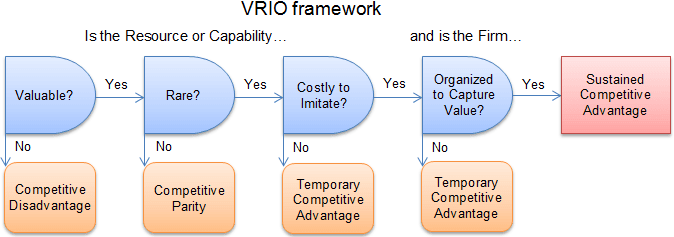
\includegraphics[width=0.8\textwidth]{vrio_framework}
 	\caption[The VRIO framework]{The VRIO framework. Adapted from~\DIFdelbeginFL \DIFdelFL{\cite{rothaermel2012strategic}}\DIFdelendFL \DIFaddbeginFL \DIFaddFL{\citep{rothaermel2012strategic}}\DIFaddendFL } \label{fig:VRIO}
\end{figure}

The VRIN framework developed in~\cite{Barney:1991ur} was also extended and improved upon~\cite{Barney:1995tz} just as he had improved on the terminology of \rbt.
\cite{Barney:1995tz} introduced the concept of \DIFdelbegin \DIFdel{VRIO.
}\DIFdelend \DIFaddbegin \acrshort{VRIO} \DIFadd{to improve on }\acrshort{VRIN}
\DIFaddend \begin{description} 
   \setlength{\itemsep}{1pt}
\item[The Question of Value] Resources are valuable if they help organisations to increase the value offered to the customers. This is done by increasing differentiation or/and decreasing the costs of the production. The resources that cannot meet this condition, lead to competitive disadvantage.

\item[The Question of Rarity] Resources that can only be acquired by one or few companies are considered rare. When more than few companies have the same resource or capability, it results in competitive parity.

\item[The Question of Imitability] A company that has valuable and rare resource can achieve at least temporary competitive advantage. However, the resource must also be costly to imitate or to substitute for a rival, if a company wants to achieve sustained competitive advantage.

\item[The Question of Organisation] The resources itself do not confer any advantage for a company if it’s not organised to capture the value from them. Only the firm that is capable to exploit the valuable, rare and imitable resources can achieve sustained competitive advantage\footnote{adopted from~\DIFdelbegin \DIFdel{\cite{Strategic-management-insight:2013}}\DIFdelend \DIFaddbegin \DIFadd{\citep{Strategic-management-insight:2013}}\DIFaddend }.
\end{description}

The key improvement to the VRIO (see also \ref{fig:VRIO}) framework from the VRIN framework is the addition of the question if the organisation is ready and capable to exploit all the resources~\DIFdelbegin \DIFdel{\cite{Barney:1995tz,Strategic-management-insight:2013}}\DIFdelend \DIFaddbegin \DIFadd{\citep{Barney:1995tz,Strategic-management-insight:2013}}\DIFaddend .
The point is that all this should again lead to~\ca through \glspl{FSA}~\DIFdelbegin \DIFdel{\cite{Barney:1991ur,Barney:2001tj,Barney:2011jp}}\DIFdelend \DIFaddbegin \DIFadd{\citep{Barney:1991ur,Barney:2001tj,Barney:2011jp}}\DIFaddend . 
The frameworks by~\cite{Barney:1991ur,Barney:1995tz} lead to the following:

\begin{WP}\DIFaddbegin \label{wp:rbt}
  \DIFaddend The diversity in internal resources (humans and knowledge) within firms could be responsible for the heterogeneity of firms responses to changes institutional environment
\end{WP}

\subsection{Firm specific resources}

A key concept of~\DIFdelbegin \DIFdel{\cite{Barney:1991ur,Barney:2001tj} }\DIFdelend \DIFaddbegin \DIFadd{\citep{Barney:1991ur,Barney:2001tj} }\DIFaddend is that the different (internal) resources lead to~\glspl{FSA}.
The resources of MNE are by definition located in the host and home country of that MNE. 
\cite{Barney:1991ur,Barney:1995tz} suggests that ``resources within the firm are not perfectly mobile across firms and that heterogeneity can be long lasting''~\DIFdelbegin \DIFdel{\cite{Barney:1991ur}}\DIFdelend \DIFaddbegin \DIFadd{\citep{Barney:1991ur}}\DIFaddend .
Whether this assumption holds true is a matter of discussion.
The fact that resources might be (perfectly) mobile given certain constraints has been brought up~\DIFdelbegin \DIFdel{\cite{Lavie:2006up,Priem:2001vd} }\DIFdelend \DIFaddbegin \DIFadd{\citep{Lavie:2006up,Priem:2001vd} }\DIFaddend already.\\
\cite{Hu:1995vg} identified that the firm's advantages are indeed transferable, be it with varying amounts of success (certain constraints).
The success are visible through the expansion of Hong Kong firms in East Asia~\DIFdelbegin \DIFdel{\cite{Hu:1995vg}}\DIFdelend \DIFaddbegin \DIFadd{\citep{Hu:1995vg}}\DIFaddend .
However these similar firms expanding to the US or Great Britain yielded a different story~\cite{Hu:1995vg}.\\
The same holds for (high-tech) Korean firms expanding to \glsfull{EE} and \glsfull{AE}. 
Here a difference strategies was observed while sill dealing with comparable MNEs~\DIFdelbegin \DIFdel{\cite{Erramilli:1997wu}}\DIFdelend \DIFaddbegin \DIFadd{\citep{Erramilli:1997wu}}\DIFaddend .
The same firm specific resources were employed in different capacities relative to the market that was entered.\\
Not only the economic regions that are entered are relevant to the methods and impact resources have on the MNE.
The type of resource has a profound effect on its capacity to be either internationally mobile or immobile~\DIFdelbegin \DIFdel{\cite{Tseng:2007wm}}\DIFdelend \DIFaddbegin \DIFadd{\citep{Tseng:2007wm}}\DIFaddend .\\
Some \fsa have in the form of resources have different characteristics in general. 
\cite{Rugman:2001ti} differentiates between three types of resources.
\begin{enumerate}[(a)]
   \setlength{\itemsep}{1pt}
\item Non location bound \fsa
\item Location bound \fsa 
\item Subsidiary specific advantages
\end{enumerate}
Where the (non) location bound \fsa are in it self to be exploited globally and easy to diffuse locally (a) or hard to exploit globally and provide local national responsiveness (b) the subsidiary specific advantages are a different animal by itself. 
They are easy to deploy globally but difficult to exploit internally~\DIFdelbegin \DIFdel{\cite{Rugman:2001ti}}\DIFdelend \DIFaddbegin \DIFadd{\citep{Rugman:2001ti}}\DIFaddend .
The subsidiary specific advantages display characteristics of perfectly mobile resources as they are very mobile across firms, but not within firms or MNEs.\\
The observations above relax the statement of~\cite{Barney:1991ur} somewhat as to the perfect mobility of resources.
According to~\DIFdelbegin \DIFdel{\cite{Rugman:2001ti,Tseng:2007wm,Erramilli:1997wu,Hu:1995vg,Rugman:1992uj} }\DIFdelend \DIFaddbegin \DIFadd{\citep{Rugman:2001ti,Tseng:2007wm,Erramilli:1997wu,Hu:1995vg,Rugman:1992uj} }\DIFaddend some consideration has to be given to the fact that resources are perfectly immobile according to \rbt.
This may not be always a certainly.
This depends off course on a case by case basis as indicated above.

%The theory of Barney is \emph{introspective}. 
%It takes into account what is happening inside the firm.
%What knowledge is available, the people matter. 
%Processes that have been created over time are a contributing factor. 
%In the 1970's Toyota engineered \gls{tpm} for it's factories this gave them \gls{CA} over their US rivals as production cost were lower for their products.
%Only if these resources cannot be imitated in an other country and location this can create a \gls{CA}.
%In contrast to~\gls{RBV} the theory of~\cite{Porter:1980to} is thus~\emph{extrospective} and does not consider the company itself.\\
%Actually both theories are not mutually exclusive. They are very well capable of existing simultaneously. 
%DIF < This line of thought give rise to the fact that there might be a third pillar in strategy thinking. %LitReview/Strategy Lit/
%DIF > This line of thought give rise to the fact that there might be a third pillar in strategy thinking.

%DIF < \section{Institutional Based View}\label{ch:peng}

Context and institutions are the prevalent terms when it comes to~\ibv. %\rbv and \inbv.
This~\ibv considers not only the firms (similar to~\cite{Porter:1980to}) and resources (similar to~\cite{Barney:1991ur}) but also engages in considering the institutional constraints.

The \ibv~dictates that firms performance and choices do not only depend on resources and the industry the firm is competing in, but also depends on the (a) environment (institutional constraints) in which managers and firms pursue their interest~\citep{Peng:2008b}.%
The institutional framework can have a positive effect on innovations (in the US for example) and a negative effect in Japan. 
In this case old drug are more profitable than new drugs in Japan~\citep{Peng:2008b}. \\
On the other hand~\ibv proposed that (b) formal and informal institutions combine to govern firm behaviour, in situations where formal constraints fail, informal constraints play a larger role in reducing uncertainty and providing consistency to managers and firms~\citep{Peng:2008b}. \\
Both effects (a) and (b) can be summarised in the word `context'. Context is the third leg~\cite{Peng:2009vt} that influences the various decisions that firms have decide on in~\ib. 
The institutions (which are part of the context) present themselves in two forms `formal' and `informal'~\citep{Peng:2002ef}. 
The latter are things like accepted social behaviour and come into play when formal constraints fail~\citep{North:1990vl,DiMaggio:1983wt,Scott:2001tt}.
The first include political rules, judicial decisions, and economic contracts. 
More on the theory of institutions will be investigated in Section~\ref{sec:InTh}.

So~\ibv~takes into account not only strategic choices driven by industry conditions and firm-specific resources, that traditional strategy research emphasises (\cite{Porter:1980to,Barney:1991ur}), but are also a reflection of the formal and informal constraints of a particular institutional framework that decision makers confront (\cite{Oliver:1997wj,Scott:2001tt}). Given the influence of institutional frameworks on firm behaviour, any strategic choice that firms make is inherently affected by the formal and informal constraints of a given institutional framework (\cite{North:1990vl,Oliver:1997wj}). 

\begin{figure}
\centering
\tikzsetnextfilename{Peng_2000}
\begin{tikzpicture}[scale=0.75, transform shape]
% STYLES
\tikzset{
    ellips/.style={ellipse, draw, minimum width=100pt,
    align=center,node distance=3cm,inner sep=5pt,text width=2.5cm,minimum    
    height=2.0cm,>=stealth}%fill=black!10
}

\node [ellips](Choices) {Strategic Choices};
\node [above=2cm of Choices](dummy) {};
\node [ellips, left=1.5cm of dummy] (Institutions) {Institutions};
\node [ellips, right=1.5cm of dummy] (Organisations) {Organisations};

% Draw the links between 
\path[<->,thick] 
   (Choices) edge node[anchor=center, text width=3.5cm, below left, midway] {Industry conditions and 
    firm-specific resources}  (Institutions) 
   (Choices) edge node[anchor=center, text width=3.5cm, below right, midway] {Formal and informal 
   constraints} (Organisations)
 (Institutions) edge  node [midway, below] {interaction} node[midway, above] {Dynamic} (Organisations);
\end{tikzpicture} 
\caption[Institutions, organisations, and strategic choices]{Institutions, organisations, and strategic choices. Source:~\cite{Peng:2000ut}}%
\label{fig:Peng2000} 
\end{figure}


So \ibv focusses not only on strategy and the firms that make these strategic choices but takes into account the institutions that govern the playing field. Moreover the interaction between the firms, institutions and the strategic choices is what \ibv~is all about.\\
Strategic literature does not discuss the specific relationship between strategic choices and institutional frameworks~\citep{Peng:2008us}.
In contrast to earlier theories,~\ibv~does not exist on it's own. It is merely an extension on earlier theories.This figure (\ref{fig:Peng2000}) shows the dependance on both the theories of~\cite{Barney:2001wq} and~\cite{Porter:1980to} for~\ibv. 
Obviously~\ibv~is not an attempt to dismiss other theories more an attempt to complete theories on strategy as they exist at the moment. 
Strategy is about making the right choices at the correct moment. 


%\tikzsetnextfilename{3rdLeg}
\begin{tikzpicture}[scale=0.7, transform shape]
% STYLES
\tikzset{
    ellips1/.style={ellipse, draw, 
    align=center, node distance=2.5cm, inner sep=5pt, >=stealth,text width=4.0cm},
  %fill=black!10,minimum ,text width=3.3cm, height=2.75cm, text width=2.9cm,
    ellips/.style={ellipse, draw, minimum width=100pt,
    align=center,node distance=3cm,inner sep=5pt, text width=2cm,   
   minimum height=1.0cm,>=stealth}%fill=black!10, 
}
\node [ellips1](Industry) {Industry-Based Competition};
\node [ellips1, below=1cm of Industry](Firm) {Firm Specific Resources and Capabilities};
\node [ellips1, below=1cm of Firm] (Institutional) {Institutional Conditions and Transitions};
\node [ellips, right=1.5cm of Firm] (Strategy) {Strategy};
\node [ellips, right=1.5cm of Strategy] (Performance) {Performance};

% Draw the links between 
\path[->,thick] 
   (Industry.east) edge  (Strategy) 
   (Firm.east) edge  (Strategy)
   (Institutional.east) edge  (Strategy)
   (Strategy) edge  (Performance);
 
\end{tikzpicture} 


\begin{figure}
\centering
%\tikzsetnextfilename{mysphere}
\tikzsetnextfilename{3rdLeg}
\begin{tikzpicture}[scale=0.7, transform shape]
% STYLES
\tikzset{
    ellips1/.style={ellipse, draw, 
    align=center, node distance=2.5cm, inner sep=5pt, >=stealth,text width=4.0cm},
  %fill=black!10,minimum ,text width=3.3cm, height=2.75cm, text width=2.9cm,
    ellips/.style={ellipse, draw, minimum width=100pt,
    align=center,node distance=3cm,inner sep=5pt, text width=2cm,   
   minimum height=1.0cm,>=stealth}%fill=black!10, 
}
\node [ellips1](Industry) {Industry-Based Competition};
\node [ellips1, below=1cm of Industry](Firm) {Firm Specific Resources and Capabilities};
\node [ellips1, below=1cm of Firm] (Institutional) {Institutional Conditions and Transitions};
\node [ellips, right=1.5cm of Firm] (Strategy) {Strategy};
\node [ellips, right=1.5cm of Strategy] (Performance) {Performance};

% Draw the links between 
\path[->,thick] 
   (Industry.east) edge  (Strategy) 
   (Firm.east) edge  (Strategy)
   (Institutional.east) edge  (Strategy)
   (Strategy) edge  (Performance);
 
\end{tikzpicture} 


\caption[The Institution-Based View as a Third Leg for a Strategy Tripod]{The Institution-Based View as a Third Leg for a Strategy Tripod. Source:~\citep{Peng:2009vt}}%
\label{fig:Peng2009} 
\end{figure}


Treating institutions as independent variables, an institution-based view on business strategy, therefore, focuses on the dynamic interaction between institutions and organisations, and considers strategic choices as the outcome of such an interaction (see figure~\ref{fig:Peng2000})~\citep{Peng:2002ef}.
Not only have more scholars come to realise that institutions matter~\citep{Powell:1991wn,Scott:2001tt}, but also that strategy research cannot just focus on industry conditions and firm resources~\citep{Khanna:1997wd}.
Although firms take decisions on the individual resources and capabilities~\cite{Barney:1991ur} the influence of institutions can no longer be ignored. This is where~\ibv extends strategic literature.
When introduced the \gls{RBV} in international business literature this view gained a lot of support. 
The theory has been expanded upon and \gls{IBV} was introduced by~\citep{Kostova:1999wt,Meyer:2009ue,Wang:2012ge}.   %LitReview/Strategy Lit/
\DIFdelbegin %DIFDELCMD < 

%DIFDELCMD < %%%
\DIFdelend \section{Conclusions}

From an theoretical standpoint the \gls{WTO} can certainly be seen as an institution.
As a rules setting body the \wto~does certainly qualify as an institution and by setting these roles it tries to reduce the uncertainty for organisations.
The institutional characteristics are certainly very visible in the Formulation Phase of the \wto~life cycle. The outcome of the institution, the result, is most visible in the Implementation phase. this is where the organisations (firms) have to respond to the new landscape. \\
Their context has changed.
This changing context is best theorised by the \gls{IBV}~and more to the point the strategy tripod~\cite{Peng:2009vt} and shown in figure~\ref{fig:Peng2009}.
The manner in which the firms respond to the changing context is not only dependant on the context, country and state and stage of the economy, but also has to do with the available resources and the industry of the firm is competing in. \\
The possible differences and similarities will be investigated in the next section.%DIF > 


\chapter{Methodology}
This chapter will focus on the research methodology and design.
Before going into the research design, the reasoning for the use of qualitative research model will be discussed.
%Secondly, the research design will be discussed of which qualitative research method is used in the form of multiple case study which will be explored to get the required information for this study. 
Then the case criteria selection and the data collection methods will be given.
%------------------------
%Waarden ophalen uit database

When doing research\DIFaddbegin \DIFadd{, }\DIFaddend two basic methods can be distinguished, qualitative and quantitative~\DIFdelbegin \DIFdel{\cite{Saunders:2009wn}}\DIFdelend \DIFaddbegin \DIFadd{\citep{Saunders:2009wn}}\DIFaddend .
when researchers try to discover causal links between two or more subjects quantitative research is deemed most appropriate~\DIFdelbegin \DIFdel{\cite{van2008management}}\DIFdelend \DIFaddbegin \DIFadd{\citep{van2008management}}\DIFaddend .
In this thesis the data will be analysed using what~\DIFdelbegin \DIFdel{\cite{Saunders:2009wn} }\DIFdelend \DIFaddbegin \DIFadd{\citep{Saunders:2009wn} }\DIFaddend refers to as `non numeric' data, hence this research study is qualitative in nature.
To determine motivations, perceptions or beliefs of a certain phenomenon~\DIFdelbegin \DIFdel{\cite{van2008management,Eisenhardt:1989ww} }\DIFdelend \DIFaddbegin \DIFadd{\citep{van2008management,Eisenhardt:1989ww} }\DIFaddend qualitative research is considered most appropriate.
The study will be done in a mono-method capacity, hence no quantitative data will be used in this research~\DIFdelbegin \DIFdel{\cite{Saunders:2009wn}}\DIFdelend \DIFaddbegin \DIFadd{\citep{Saunders:2009wn}}\DIFaddend .
The qualitative case study methodology provides tools for researchers to study complex phenomena within their contexts~\DIFdelbegin \DIFdel{\cite{Baxter:2008vu,Ryan:2003hn}}\DIFdelend \DIFaddbegin \DIFadd{\citep{Baxter:2008vu,Ryan:2003hn}}\DIFaddend .\\
\DIFdelbegin %DIFDELCMD < 

%DIFDELCMD < %%%
\DIFdelend %Amongst all philosophical assumptions reviewed, the interpretive paradigm has been identified as the most appropriate framework to use for this study~\cite{Yin:2009vh}. 
\DIFaddbegin \section{\DIFadd{Multiple Case Study Research Design}}
\DIFaddend 

\DIFdelbegin \section{\DIFdel{Multiple Case Study research design}}
%DIFAUXCMD
\addtocounter{section}{-1}%DIFAUXCMD
%DIFDELCMD < 

%DIFDELCMD < %%%
\DIFdelend The research design explains the structure of research. 
In fact, it explains how research is conducted and how the subsequent data is analysed~\DIFdelbegin \DIFdel{\cite{van2008management}}\DIFdelend \DIFaddbegin \DIFadd{\citep{van2008management}}\DIFaddend .
To collect the (qualitative) data for this study the method of the multiple case study has been selected.\\
According to~\cite{Yin:2009vh} case studies differentiate from other types of studies in that an attempt is made to examine a contemporary phenomenon within a real-life context. 
The technique of case studies is mostly employed when there are no clear boundaries between that particular phenomenon and it’s context~\DIFdelbegin \DIFdel{\cite{Yin:2009vh,Marshall:1996wc}}\DIFdelend \DIFaddbegin \DIFadd{\citep{Yin:2009vh,Marshall:1996wc}}\DIFaddend .
Clearly the effects of the WTO on \gls{IB} and the firms within the \gls{IB} environment are a real-life current phenomenon. 

The multiple case study differs from the single case study~\DIFdelbegin \DIFdel{\cite{van2008management,Yin:2009vh}}\DIFdelend \DIFaddbegin \DIFadd{\citep{van2008management,Yin:2009vh}}\DIFaddend .
The single case study is often used when dealing with an exceptional situation, where the multiple case study deals more than one case, having the benefit replication across cases~\DIFdelbegin \DIFdel{\cite{Saunders:2009wn}}\DIFdelend \DIFaddbegin \DIFadd{\citep{Saunders:2009wn}}\DIFaddend .
The (qualitative) multiple case study is an approach to research that facilitates exploration of a phenomenon within its context using a variety of data sources~\DIFdelbegin %DIFDELCMD < \pcite{Baxter:2008vu}%%%
\DIFdelend \DIFaddbegin \DIFadd{\citep{Baxter:2008vu}}\DIFaddend .
This ensures that the issue is not explored through one lens, but rather a variety of lenses, which allows for multiple facets of the phenomenon to be revealed and understood~\DIFdelbegin %DIFDELCMD < \pcite{Baxter:2008vu}%%%
\DIFdelend \DIFaddbegin \DIFadd{\citep{Baxter:2008vu}}\DIFaddend .
This is an approach to research that facilitates exploration of a phenomenon within its context using a variety of data sources~\DIFdelbegin \DIFdel{\cite{Baxter:2008vu}}\DIFdelend \DIFaddbegin \DIFadd{\citep{Baxter:2008vu}}\DIFaddend .\\
The advantage of this method is, it assures a richness of content, as~\cite{Eisenhardt:1989ww} explains and can lead to novel, testable and rich information.\\
%The \mcs approach can lead to novel, testable and rich information.
However, the disadvantage of this method is that the results are not statistically generalisable~\DIFdelbegin \DIFdel{\cite{Yin:1981wc}}\DIFdelend \DIFaddbegin \DIFadd{\citep{Yin:1981wc}}\DIFaddend .  
By investigating a phenomenon at one particular location, cross-sectionally and with only few organisations within the sample as units of analysis, this would result in lower generalisability~\DIFdelbegin \DIFdel{\cite{Klossek:2012wc}}\DIFdelend \DIFaddbegin \DIFadd{\citep{Klossek:2012wc}}\DIFaddend . 
The results are only valid in a specific setting for specific type of organisations~\DIFdelbegin \DIFdel{\cite{Deng:2007tr}}\DIFdelend \DIFaddbegin \DIFadd{\citep{Deng:2007tr}}\DIFaddend .
This research method aims to describe, rank and explore data with the aim of generating working propositions or illustrating an existing theory~\DIFdelbegin \DIFdel{\cite{Eisenhardt:1989ww,Yin:1981wc}}\DIFdelend \DIFaddbegin \DIFadd{\citep{Eisenhardt:1989ww,Yin:1981wc}}\DIFaddend .\\
The multiple case study can been seen as the ideal method of collecting data and or information for this research question~\DIFdelbegin \DIFdel{\cite{Yin:2009vh}}\DIFdelend \DIFaddbegin \DIFadd{\citep{Yin:2009vh}}\DIFaddend .
This thesis is investigating two different regions of the world based on the economic development of that area (\glspl{EE} vs. \glspl{AE} see also Appendix~\ref{app:AEnEE}) and also two different industries in these economic areas, the \pharma and ICT services industries that are governed by WTO \rr. 
The rationale behind the choice of these two industries and specific companies is explained in Section~\ref{sec:rational}.
%By investigating a certain phenomenon at only one particular location, cross-sectionally and with only a few organisations within the sample as units of analysis, this could result in lower generalisability (Klossek et al, 2012; Deng, 2007). 
%On has to keep track of the fact that the results are only valid in a combination of specific settings and organisations.

This research method aims to discover not as much explanatory, but moreover exploratory findings~\cite{Yin:1981wc} on the effects of the WTO \rr.
The `why' question for~\mcs is associated with explanatory research questions~\cite{Yin:2009vh}, this thesis does not seek to answer those.
Here the question is whether the WTO effects some companies in certain countries or regions differently. 
Hence the research question is an exploratory one~\DIFdelbegin \DIFdel{\cite{Yin:2009vh,Miles:1994wi}}\DIFdelend \DIFaddbegin \DIFadd{\citep{Yin:2009vh,Miles:1994wi}}\DIFaddend .\\
In this research, the propositions were developed prior to carrying out the case study research. 
This is in line with~\DIFdelbegin \DIFdel{\cite{Yin:2009vh,Hyde:2000hf} }\DIFdelend \DIFaddbegin \DIFadd{\citep{Yin:2009vh,Hyde:2000hf} }\DIFaddend (multiple) case study approach.

\section{Case \DIFdelbegin \DIFdel{criteria }\DIFdelend \DIFaddbegin \DIFadd{Criteria }\DIFaddend and \DIFdelbegin \DIFdel{selection}\DIFdelend \DIFaddbegin \DIFadd{Selection}\DIFaddend }

The next step is to identify and select the cases that will be used. 
As mentioned by~\cite{Pettigrew:1990}, the number of cases that are studied is usually limited, therefore it is a good approach to select cases that signify correctly the differences at hand.
%The research approach aims to obtain in this way exploratory, as well as explanatory findings. The exploratory element would refer to how some variables might influence the degree of knowledge sharing; the explanatory element would provide insight in how some variables should be adjusted in order to enhance inter- business unit knowledge sharing for multi-domestic MNEs (Yin, 2012).
In the selection process certain boundaries have been set to ensure a comprehensive selection can be made.
The selection of the firms will be make on a number differentiating levels.
The first differentiating level will be economic region.
The second will be on type of industry.

\subsection{Economic \DIFdelbegin \DIFdel{region selection}\DIFdelend \DIFaddbegin \DIFadd{Region Selection}\DIFaddend }

The aim of this study is to compare the effects of the \gls{WTO} decisions on  \gls{EE} and \gls{AE} firms.
Hence the cases will be selected from \gls{EE} and \gls{AE} firms.
The terms \gls{EE} and \gls{AE} have been defined in Appendix~\ref{app:AEnEE} and the specific economic regions or countries associated with the \gls{EE} and \gls{AE} are also listed in this Appendix.

The region that has been selected as \gls{AE} is the European Union. 
To create a larger potential group of firms (MNEs) the \gls{EU} has been selected as opposed to a single european country.
As this thesis is written in a European environment is seems only logical to choose Europe as the \gls{AE}.

As for a \gls{EE} a number of choices as possible.
The obvious choice in this case would be China a there is already there is a lot of research being done with China and Chinese MNEs.
However India does make for a very interesting candidate.
The exposure India as a country and economic power receives might be less.
The Economist does have a separate section on China but does not have one on India for example.
Looking at the 2012 \gls{GDP} of both India and China they rank 4th and 3rd respectively (with the EU and the US in 1st and 2nd)~\DIFdelbegin \DIFdel{\cite{CIA:2013}}\DIFdelend \DIFaddbegin \DIFadd{\citep{CIA:2013}}\DIFaddend .
India does have a well established services sector contributing over 50\% to \gls{GDP}~\DIFdelbegin \DIFdel{\cite{Government-of-India:2012}}\DIFdelend \DIFaddbegin \DIFadd{\citep{Government-of-India:2012}}\DIFaddend .
India be less known as a manufacturer as China~\cite{Daily-Mail:2010}, it does have a lot of potential~\DIFdelbegin \DIFdel{\cite{Dhawan:2012ws}}\DIFdelend \DIFaddbegin \DIFadd{\citep{Dhawan:2012ws}}\DIFaddend .\\
Therefor India is a very interesting \gls{EE} and has dully been selected.

%Viewed from a global point of view, the influence of the \wto~spans the entire globe. 
%This playing field is than decided into two economic blocks: \gls{EE} and \gls{DE}. 
%As these two blocks span a great number of countries and continents, India (an \gls{EE}) and the \gls{EU} have been chosen to represent the two economic blocks. 
%Both India and the EU have an equally long standing relation with the \wto~and have been active in the various life cycles of the \wto~for a great number of years.\\
%The next level of distinction that can be determined is the industry level. 
%Within both the EE and DE one can find different industry types.

\subsection{Industry \DIFdelbegin \DIFdel{selection}\DIFdelend \DIFaddbegin \DIFadd{Selection}\DIFaddend }\label{sec:rational}

In~\cite{Porter:1980to} already identified the importance of industries in the search for~\ca. 
The industry types have to be existent in sufficient quantities in both economic blocks.
For a good comparison looking at different industry types seems logical. \\
\cite{Fisher:1939} defined three industry sectors; the Primary, Secondary and Tertiary sectors.
The primary sector consists mainly of raw material sourcing companies, the secondary sector has to do with manufacturing and the tertiary sector consists of services firms.
For the purpose of this research we will focus on firms from the secondary and tertiary sectors~\DIFdelbegin \DIFdel{\cite{Fisher:1939}}\DIFdelend \DIFaddbegin \DIFadd{\citep{Fisher:1939}}\DIFaddend .
%To be able to make an accurate comparison, firms that will be chosen have to be present in both industries and in both the European Union and India.


\subsubsection{Manufacturing Industry} 

%For the manufacturing industry, the pharmaceutical industry has been selected.
To be able to come to a comprehensive comparison, the sectors under investigation are to be both present in the \gls{EE} and the \gls{AE} alike. 
This is the case for the \pharma industry in both \gls{EU} and in India.\\
The pharmaceutical has been long present in the EU\DIFaddbegin \@\DIFaddend . 
Especially Germany, Switzerland and Britton have a history (dating back to the 18th century) in the pharmaceutical business~\DIFdelbegin \DIFdel{\cite{Walsh:2010,Liebenau:1984wb}}\DIFdelend \DIFaddbegin \DIFadd{\citep{Walsh:2010,Liebenau:1984wb}}\DIFaddend .
Although not as old as the European history, India does have a history in the \pharma industry~\DIFdelbegin \DIFdel{\cite{Mazumdar:2013vr}}\DIFdelend \DIFaddbegin \DIFadd{\citep{Mazumdar:2012tx}}\DIFaddend . 

Not of primary concern, but still useful, the \pharma sector has decent size firms in both \gls{EU} and India.
Hence the amount of information is expected to be sufficiently available on companies in these regions and sectors.


\subsubsection{Services Industry} 


As a service the~\gls{IT} services industry is very much on the move and an example of the globalisation of the workplace~\DIFdelbegin \DIFdel{\cite{Reuters:2012}}\DIFdelend \DIFaddbegin \DIFadd{\citep{Reuters:2012}}\DIFaddend . 
Development centres are being set up all over the world~\DIFdelbegin \DIFdel{\cite{Reuters:2012,India-Times:2008}}\DIFdelend \DIFaddbegin \DIFadd{\citep{Reuters:2012,India-Times:2008}}\DIFaddend . 
As for the services industry, India is well known for their ICT services industry. 
One can almost argue that India has a leading role in the~\gls{IT} services and~\gls{BPO} practices~\DIFdelbegin \DIFdel{\cite{The-Hindu:2011}}\DIFdelend \DIFaddbegin \DIFadd{\citep{The-Hindu:2011}}\DIFaddend . 
The I(C)T services industry is one of the largest Industries of India. 
It accounts for 41.7\% of the total services export~\DIFdelbegin \DIFdel{\cite{Government-of-India:2012}}\DIFdelend \DIFaddbegin \DIFadd{\citep{Government-of-India:2012}}\DIFaddend .
One can conclude the~\gls{IT} services industry is well established in India and could be solid choice as a services industry example.

In Europe and the~\gls{EU} the~\gls{IT} services firms do not see the same amount of growth as the Indian industry however there are still some large companies active~\DIFdelbegin \DIFdel{\cite{Deloitte:2010}}\DIFdelend \DIFaddbegin \DIFadd{\citep{Deloitte:2010}}\DIFaddend . 
Much of the~\gls{IT} services is about outsourcing~\gls{IT} work\footnote{More on the working practices of the~\gls{IT} services industry can be found in~\ref{sec:sevicesFirms}}.
For this reason all~\gls{IT} services firms have a global presence and a lot of the actual (coding) work is done in low-wage countries (like India). 
Notwithstanding this globalisation aspect, Europe boasts still healthy number if~\gls{IT} services companies~\cite{Computer-Weekly:2011} that can be used in this thesis.
From this on can conclude that overall the~\gls{IT} services industry in Europe is still a healthy one to serve as a services industry example.

%Distance is not a factor when it comes to delivering a ~\gls{IT} solution.
%One can send an application across half the world in a matter of seconds. 
Both the~\gls{IT} services and \pharma industries seem interesting industries to focus on, with regard to the services they provide and in the light of the division in industries as defined by~\DIFdelbegin \DIFdel{\cite{Fisher:1939}}\DIFdelend \DIFaddbegin \DIFadd{\citep{Fisher:1939}}\DIFaddend .


\subsubsection{Firms}

Finally within these industries defined, the firms can to be selected. 
To be able to find as much information as possible multinational \pharma companies have been selected from both the European and Indian markets.\\
The Indian \pharma companies are Ranbaxy and Cipla.\\ %(possibly Dr Reddy's).
The choice of these two companies is base on the size, they are among the largest in India and have a decent amount of growth (see Figure~\ref{fig:IndiaPharma}).

\begin{figure}[htbp] 
	\centering
	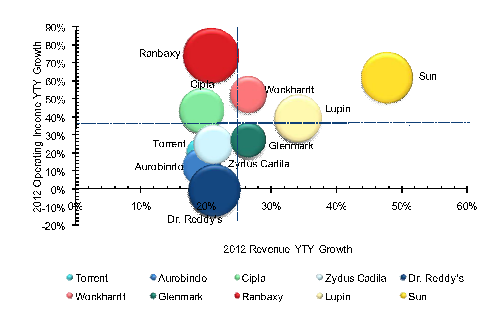
\includegraphics[width=0.8\textwidth]{IndiaPharma.eps}
 	\DIFdelbeginFL %DIFDELCMD < \caption[Competitive Landscape of the Top 10 Pharmaceutical Companies in India, 2012]{%%%
\DIFdelendFL \DIFaddbeginFL \caption[Competitive Landscape of the Top 10 Pharmaceutical Companies in India]{\DIFaddendFL Competitive Landscape of the Top 10 Pharmaceutical Companies in India, 2012. source:~\DIFdelbeginFL \DIFdelFL{\cite{Research-and-Markets:2013}}\DIFdelendFL \DIFaddbeginFL \DIFaddFL{\citep{Research-and-Markets:2013}}\DIFaddendFL }\label{fig:IndiaPharma}
\end{figure}

Many European \pharma companies have merged with or have been purchased by US firms. 
We will focus on firms that have no original ties with the US through mergers and that stem from the European mainland.
As counterparts for the Indian firms we will choose Novartis and GSK as the European contenders.
Both the European firms are top 20 of \pharma~companies\footnote{\url{http://www.contractpharma.com/issues/2013-07/view_features/top-20-pharma-report-/}} in the world.\\
As for the ICT services firms in India there is a lot of choice. 
Here we opt for pure Indian companies were not only the operations are performed in India but the management and ownership are also Indian.
Here Infosys and WiPro have been chosen. 
%(TCS) is used as a backup company as they are not purely a ICT company.
Both companies are among the largest~\gls{IT} services firms in India feature in Gartner's Magic Quadrant for~\gls{IT} services firms~\cite{Gartner:2013a} and not a subsidiary from a larger company.
This would be the fact with TCS as this is part of the Tata group.

For the European Firms the choice is less broad. 
Pure European ICT firm are not as prevalent as Indian ICT services firms~\DIFdelbegin \DIFdel{\cite{Deloitte:2010}}\DIFdelend \DIFaddbegin \DIFadd{\citep{Deloitte:2010}}\DIFaddend . 
This said Capgemini and T-systems as well as Atos are all very good examples of international ICT services firm. 
There are a number of local (national) ICT services for a good diversity of information these are not included.\\
Here the choice is Capgemini and T-systems as they again rank among the largest companies in this field in Europe.
T-systems and Capgemini have roots in different European countries~\DIFdelbegin \DIFdel{\cite{capgemini:2013aa,T-systems:2013} }\DIFdelend \DIFaddbegin \DIFadd{\citep{capgemini:2013aa,T-systems:2013} }\DIFaddend (France and Germany) this could provide an additional richness of data.\\
The firms in their respected economic areas and industries will be summarised in table~\ref{tab:firms}.

\begin{table}
  \centering
  \caption[Firms of under investigation]{Firms of under investigation. Source Author}\label{tab:firms}%
\begin{tabularx}{0.6\textwidth}{lXX} 
 % \toprule
 & \de (EU)& \ee (India)\\ 
  %\midrule 
  \midrule
  Services & Capgemini& Infosys \\
Industry  &T-Systems&WiPro\\
   \midrule
 Manufacturing &Novatis&Ranbaxy\\
 Industry &GSK & Cipla\\
  \bottomrule
  \end{tabularx}
\end{table}

The Firms will be described in more detail in the following section.

\paragraph{Detailed description of the firms}\label{sec:sevicesFirms}

The way~\gls{IT} services firms operates within the~\gls{IT} services business is largely the similar for Indian or European firms~\cite{Gardner:2013}. 
Therefor these working practices are described for the entire sector and not repeated in table~\ref{tab:ServfirmsDescriptions}.
\DIFdelbegin %DIFDELCMD < \\%%%
\DIFdel{~}\DIFdelend \gls{IT} services firms generally provide~\gls{IT} maintenance and development through outsourcing (in near or offshore locations) and~\gls{BPO} services~\DIFdelbegin \DIFdel{\cite{Wipro:2013aa,Infosys:2013aa,capgemini:2013aa,T-systems:2013}}\DIFdelend \DIFaddbegin \DIFadd{\citep{Wipro:2013aa,Infosys:2013aa,capgemini:2013aa,T-systems:2013}}\DIFaddend . 

The majority of \mne~have their own (proprietary)~\gls{IT} application landscape that is vital to their operations~\DIFdelbegin \DIFdel{\cite{Willcocks:2004ce}}\DIFdelend \DIFaddbegin \DIFadd{\citep{Willcocks:2004ce}}\DIFaddend . 
As part of the application management services,~\gls{IT} services firms can maintain the current~\gls{IT} application landscape and also develop new applications (or replace applications build with old technology) that are specifically tailored for their clients~\DIFdelbegin \DIFdel{\cite{Cusumano:2008ta}}\DIFdelend \DIFaddbegin \DIFadd{\citep{Cusumano:2008ta}}\DIFaddend .
The~\gls{IT} services firms typically, by acquiring the account to maintain and develop the~\gls{IT} applications also take over part of the personnel that was working at the parent company. 
Subsequently (a large) part of the development work done, is transferred to low-wage-countries~\DIFdelbegin \DIFdel{\cite{Barthelemy:2001ui}}\DIFdelend \DIFaddbegin \DIFadd{\citep{Barthelemy:2001ui}}\DIFaddend . 
The employees of these companies are located both in the home country of the client and in the home country of the~\gls{IT} services firms~\DIFdelbegin \DIFdel{\cite{Lacity:2009dk}}\DIFdelend \DIFaddbegin \DIFadd{\citep{Lacity:2009dk}}\DIFaddend .
This trend that has been observed is that these companies want to focus on their core business~\DIFdelbegin \DIFdel{\cite{Willcocks:2004ce}}\DIFdelend \DIFaddbegin \DIFadd{\citep{Willcocks:2004ce}}\DIFaddend . 
As~\gls{IT} is not their core business they outsource this to other companies or set up a second company to perform these services~\DIFdelbegin \DIFdel{\cite{Earl:2012vd}}\DIFdelend \DIFaddbegin \DIFadd{\citep{Earl:2012vd}}\DIFaddend . 
Firms that are more heavily~\gls{IT} reliant are telecommunications and financial services firms~\DIFdelbegin \DIFdel{\cite{Gonzalez:2006eh}}\DIFdelend \DIFaddbegin \DIFadd{\citep{Gonzalez:2006eh}}\DIFaddend . 
Some~\gls{IT} services firms started life as subsidiary that is operating (semi) independently, this is the case with T-Systems or have a spin-of company that is now competing in the market on its own~\DIFdelbegin \DIFdel{\cite{T-systems:2013}}\DIFdelend \DIFaddbegin \DIFadd{\citep{T-systems:2013}}\DIFaddend . 
Others started out as pure~\gls{IT} firms that have grown to become~\gls{IT} services firms partly by insourcing employees from their (former) customers~\DIFdelbegin \DIFdel{\cite{Barthelemy:2001ui}}\DIFdelend \DIFaddbegin \DIFadd{\citep{Barthelemy:2001ui}}\DIFaddend . 
The firms in the~\gls{IT} services area are described in table~\ref{tab:ServfirmsDescriptions}.

%\newpage
\begin{sidewaystable}
  %\tablefootnote{}
  \centering
  \caption[Services Firm Details]{Services Firm Details. Source \DIFdelbegin \DIFdel{: }\DIFdelend Author}\label{tab:ServfirmsDescriptions}%
   \footnotesize
\begin{tabular}{lp{4cm}p{4cm}p{4cm}p{4cm}} 
 % \toprule

 \textbf{FirmName} 
& 
\includegraphics[width=.14\textwidth]{capgemini_logo.eps}      
& 
\includegraphics[width=.145\textwidth]{T-systems_logo.eps} 
& \DIFdelbegin %DIFDELCMD < \includegraphics[width=.08\textwidth]{wipro_logo.eps} 
%DIFDELCMD < %%%
\DIFdelend \DIFaddbegin \includegraphics[width=.08\textwidth]{wipro_logo_BB.eps} 
\DIFaddend & 
\includegraphics[width=.08\textwidth]{infosys_logo.eps}\\

 \textbf{Economy}             & \glsdesc{AE}           & \glsdesc{AE}   & \glsdesc{EE}  & \glsdesc{EE}\\

 \textbf{Industry Type}     & \DIFdelbegin %DIFDELCMD < \multicolumn{4}{c}{ICT Services}%%%
\DIFdelend \DIFaddbegin \DIFadd{ICT Services     }& \DIFadd{ICT Services }& \DIFadd{ICT Services }& \DIFadd{ICT Services}\DIFaddend \\

 \textbf{Home Country}       & France         & Germany & India   & India\\

 \textbf{Employees}          & 100.000+       &  48.000 & 135.000 &150,000+\\

  \DIFaddbegin \DIFadd{\textbf{Year Founded}   }& \DIFadd{1967   }& \DIFadd{2000  }& \DIFadd{1945 }& \DIFadd{1981}\\

 \DIFaddend \textbf{Revenue (2012)}     & \euro~\DIFdelbegin \DIFdel{10Bn   }\DIFdelend \DIFaddbegin \DIFadd{10.26Bn     }\DIFaddend & \euro~\DIFdelbegin \DIFdel{9Bn 
 }\DIFdelend \DIFaddbegin \DIFadd{10.02Bn 
 }\DIFaddend & \euro \DIFaddbegin \pgfmathdivide{337.340}{\ExRupee} \pgfmathprintnumber[precision=2]{\pgfmathresult}\DIFadd{Bn}\tablefootnote{revenue was posted as \rupee~(337.340Bn) using table~\ref{tab:currencies} Euro value was calculated} 
 & \euro \DIFaddend \pgfmathdivide{433.608}{\ExRupee} \pgfmathprintnumber[precision=2]{\pgfmathresult}Bn\tablefootnote{revenue was posted as \rupee~(433.608Bn) using table~\ref{tab:currencies} Euro value was calculated}\DIFaddbegin \\

 \DIFadd{\textbf{Profit\footnote{EBITDA} (2012)} }\DIFaddend &\euro\DIFdelbegin %DIFDELCMD < \pgfmathdivide{337.340}{\ExRupee} %%%
\DIFdelend \DIFaddbegin \DIFadd{~829Mn }&\euro\DIFadd{~350Mn 
 }&
 \euro \pgfmathdivide{74.142}{\ExRupee} \DIFaddend \pgfmathprintnumber[precision=2]{\pgfmathresult}Bn\DIFdelbegin %DIFDELCMD < \tablefootnote{revenue was posted as \rupee~(337.340Bn) using table~\ref{tab:currencies} Euro value was calculated}%%%
\DIFdelend \DIFaddbegin \tablefootnote{revenue was posted as \rupee~(74.142Bn) using table~\ref{tab:currencies} Euro value was calculated} 
 &
 \euro \pgfmathdivide{100.61}{\ExRupee} \pgfmathprintnumber[precision=2]{\pgfmathresult}\DIFadd{Bn}\tablefootnote{revenue was posted as \rupee~(100.61Bn) using table~\ref{tab:currencies} Euro value was calculated} \DIFaddend \\
 \DIFaddbegin 

 \DIFaddend \midrule
 \textbf{Description} &

Capgemini is a listed company at the Euronext stock exchange in Paris. The  main business of Capgemini are ICT and consulting services. The latter was acquired via a takeover of Ernst\& Young Consulting. \newline The name came to be from a merger between CAP, Sogeti and Gemini inc. Now Sogeti is wholly owned daughter of Capgemini. Typical clients are found in large manufacturing companies, banking and insurance, but also the public sector and healthcare.  &

 T-systems is a subsidiary of Deutsche Telekom AG\@. 
 Although a subsidiary it does serve other customers than DT\@. 
 The main activities are~\gls{IT} consulting and~\gls{IT} services. 
 These include minting the~\gls{IT} application landscape and building new applications specific for the client. 
 Typical clients are found in large manufacturing companies, banking and insurance, but also the public sector. &

WiPro is an Indian ICT services company, that unlike others started of as an company that manufactured oils, soaps and waxes as the `Western India Vegetable Products'.
 This heritage is still maintained in its company logo of a sunflower. 
In 1981 WiPro diversifies into~\gls{IT} services. The business is now known for. \newline 
Their main clients other \glspl{MNE}~that are located in the financial services, healthcare, manufacturing and telecommunications domains. \DIFdelbegin %DIFDELCMD < \\
%DIFDELCMD < %%%
\DIFdelend \DIFaddbegin &
\DIFaddend In 1981 Infosys Consultants was established. In 1992 the name was changes to Infosys Technologies. Infosys is a NYSE listed global consulting and~\gls{IT} services company stemming from India. 
Similar to other Indian~\gls{IT} services firms the clients are \glspl{MNE}~that are located in the financial services, healthcare, manufacturing and telecommunications domains \\
  \bottomrule 
  \end{tabular}
\end{sidewaystable}



In general in the pharmaceutical business one can distinguish four phases in the process of the drug to hitting the market.
The drug has to be researched (a) and than (b) developed, then is has to be manufactured (c) and finally it has to be marketed and sold (d)~\DIFdelbegin \DIFdel{\cite{Paul:2010ff}}\DIFdelend \DIFaddbegin \DIFadd{\citep{Paul:2010ff}}\DIFaddend . 
The research and development stages are among the most cash intensive to the process to come up with a new (blockbuster) drug~\DIFdelbegin \DIFdel{\cite{Munos:2009bg}}\DIFdelend \DIFaddbegin \DIFadd{\citep{Munos:2009bg}}\DIFaddend .
The drugs have to be approved by the appropriate authorities\footnote{These are the \gls{FDA} in the US and the \gls{EMA} in Europe}. 
Manufacturing and marketing of the drug can begin only after this approval has been received~\DIFdelbegin \DIFdel{\cite{Kessel:2011go}}\DIFdelend \DIFaddbegin \DIFadd{\citep{Kessel:2011go}}\DIFaddend .\\
Normally a drug that has been newly developed will also be granted a patent for a certain number of years. 
After this patent expires the drug can be \manu by anyone~\DIFdelbegin \DIFdel{\cite{Kaitin:2009dg}}\DIFdelend \DIFaddbegin \DIFadd{\citep{Kaitin:2009dg}}\DIFaddend .
This dug becomes a so-called generic drug. 
Manufacturing generic drugs can might have different implications from manufacturing proprietary drugs~\DIFdelbegin \DIFdel{\cite{Kessel:2011go}}\DIFdelend \DIFaddbegin \DIFadd{\citep{Kessel:2011go}}\DIFaddend .

Indian \pharma companies have seen tremendous growth between 1970 and 1991~\DIFdelbegin \DIFdel{\cite{Chaturvedi:2006da,Bruche:2011uf}}\DIFdelend \DIFaddbegin \DIFadd{\citep{Chaturvedi:2006da,Bruche:2011uf}}\DIFaddend .
In 1970 the Patent Act was passed, which allowed the domestic manufacturing and marketing of patented products without a licence.
This fuelled a large reverse-engineering spree of patented drug by (almost all) Indian \pharma companies~\DIFdelbegin \DIFdel{\cite{Bruche:2011uf}}\DIFdelend \DIFaddbegin \DIFadd{\citep{Bruche:2011uf}}\DIFaddend .
This practice was halted in 1991 with the signing of~\gls{trips}. 
\gls{trips} marked the \DIFdelbegin \DIFdel{turningpoint }\DIFdelend \DIFaddbegin \DIFadd{turning point }\DIFaddend of Indian policy regime towards the world~\DIFdelbegin \DIFdel{\cite{Chaturvedi:2006da}}\DIFdelend \DIFaddbegin \DIFadd{\citep{Chaturvedi:2006da}}\DIFaddend .
The reverse engineering practices came to a halt. 
The new patent regime that did not allow reverse engineering of known molecules, together with the pressure exerted by liberalisation and globalisation, is forcing firms to transform their R\&D activities and realign their competencies~\DIFdelbegin \DIFdel{\cite{Chaturvedi:2006da}}\DIFdelend \DIFaddbegin \DIFadd{\citep{Chaturvedi:2006da}}\DIFaddend .

%\newpage
\begin{sidewaystable}
  \centering
  \caption[Manufacturing Firm Details]{Manufacturing Firm Details. Source Author}\label{tab:ManfirmsDescriptions}
   \footnotesize
\begin{tabular}{lp{3cm}p{3cm}p{5.5cm}p{4.3cm}}  
 \textbf{Firm Name}           & 
\includegraphics[width=.12\textwidth]{novartis_logo.eps}    & 
\includegraphics[width=.12\textwidth]{gsk_logo.eps}   &  \includegraphics[width=.13\textwidth]{ranbaxy_logo2}    &\DIFdelbegin %DIFDELCMD < 
\includegraphics[width=.09\textwidth]{cipla_logo.jpg}%%%
\DIFdelend \DIFaddbegin \includegraphics[width=.09\textwidth]{Cipla_Logo.jpg}\DIFaddend \\
 \toprule
 \textbf{Economy}             & \de          & \de   & \ee  & \ee\\

 \textbf{Industry Type}     &  \manu     & pharma \manu & pharma \manu & pharma \manu\\

 \textbf{Home Country}    & Switzerland             & UK & India& India\\

 \textbf{Employees}          & 120.000+       &  95.000 & 10.000+ &16,000+\\

 \DIFaddbegin \DIFadd{\textbf{Year Founded}    }& \DIFadd{pre 1900    }&\DIFadd{pre 1900  }& \DIFadd{1961   }& \DIFadd{1935 }\\

 \DIFaddend \textbf{Revenue (in 2012)}             
 &
 \euro~\pgfmathdivide{56.7}{\ExDollar} \pgfmathprintnumber[precision=2]{\pgfmathresult}Bn\tablefootnote{revenue was posted as \$~56.7Bn  using table~\ref{tab:currencies} Euro value was calculated}
   &
 \euro~\pgfmathdivide{26}{\ExPound} \pgfmathprintnumber[precision=2]{\pgfmathresult}Bn
\tablefootnote{revenue was posted as \pounds~26Bn  using table~\ref{tab:currencies} Euro value was calculated}
 &
 \euro \pgfmathdivide{123}{\ExRupee} \pgfmathprintnumber[precision=2]{\pgfmathresult}Bn
\tablefootnote{revenue was posted as \rupee 123Bn using table~\ref{tab:currencies} Euro value was calculated}
 &
 \euro \pgfmathdivide{85.24}{\ExRupee} \pgfmathprintnumber[precision=2]{\pgfmathresult}Bn
\tablefootnote{revenue was posted as \rupee 85.24Bn using table~\ref{tab:currencies} Euro value was calculated} 
 \\
 \DIFdelbegin %DIFDELCMD < 

%DIFDELCMD <  %%%
\DIFdelend %DIF > total operating profit
\DIFaddbegin \DIFadd{\textbf{Profit (in 2012)}   }&\euro\DIFadd{~}\pgfmathdivide{11.511}{\ExDollar} \pgfmathprintnumber[precision=2]{\pgfmathresult}\DIFadd{Bn  
}& 
\euro\DIFadd{~}\pgfmathdivide{7.4}{\ExPound} \pgfmathprintnumber[precision=2]{\pgfmathresult}\DIFadd{Bn
}&
 \euro \pgfmathdivide{(-1642.83}{\ExRupee} \pgfmathprintnumber[precision=2]{\pgfmathresult}\DIFadd{Mn
  }&
  \euro \pgfmathdivide{122.4}{\ExRupee} \pgfmathprintnumber[precision=2]{\pgfmathresult}\DIFadd{Bn}\\
 \DIFaddend \midrule
 \textbf{Description} &

Novartis is the product of a merger between Ciba-Geigy and Sandoz Laboratories in 1996. In this merger the \pharma devisions continued operation under the name Novartis while the other operations were divested. Novartis engages in research, development, manufacturing and marketing of prescription (proprietary) drugs. These four stages mentioned earlier.
\cite{businessweek:Novartis}

&
GlaxoSmithKline in full or GSK, was formed through a merger of Glaxo Wellcome and SmithKline Beecham in 2000. GSK has a portfolio of products for major diseases and also a large consumer healthcare division. GSK engages  research, development, manufacturing and marketing of prescription and over-the-counter drugs.
\cite{Businessweek:GSK}
&
Ranbaxy was founded in 1937 as a distributor of Japanese manufactured drugs. 
The name Ranbaxy is a aggregation of the names of its first owners \textbf{Ran}bir and Gur\textbf{bax}.   
In 2008 Daiichi Sankyo of Japan acquired a controlling share in Ranbaxy.
Ranbaxy however remains listed on the Indian stock exchange. 
\newline
In later stages Ranbaxy developed~\gls{ndds} techniques, thereby adding their own value to the existing products.
There is an tendency though seen at Ranbaxy to seriously pursue new drug discovery programmes. It is suggested that Ranbaxy, generally,  has been investing more in the R content of R\&D and have gradually moved away from reverse engineering~\cite{Chaturvedi:2006da}.
However the bulk of the Ranbaxy business lies in manufacturing, marketing (and selling) pharmaceuticals products\cite{Businessweek:Ranbaxy,maheshsundar:2013}
&
Cipla was founded as the Chemical, Industrial and Pharmaceutical Laboratories in 1935. 
Nowadays it is better known as its acronym then by its full name.
 Cipla \manu OTC prescriptions drugs. 
 Next to this they also manufacture \gls{API} and drug intermediates. 
 \newline 
Cipla is engaged in manufacture and marketing (sales) of pharmaceutical products in India and internationally.
Cipla focusses on improving their manufacturing efficiency and establishing large production facilities. Cipla has invested more in the D content and have strengthened their infrastructure and financial position through process efficiencies, economies of scale and large product baskets rather than research\cite{Chaturvedi:2006da}.\\
  \bottomrule 
  \end{tabular}
\end{sidewaystable}

%\subsection{WTO and the environment change}
\DIFdelbegin %DIFDELCMD < 

%DIFDELCMD < \newpage
%DIFDELCMD < %%%
\DIFdelend %DIF > \newpage
\section{Data Collection}

Since a \mcs method will be used, the data is sourced from \DIFdelbegin \DIFdel{mayor newspapers.
}\DIFdelend \DIFaddbegin \DIFadd{major newspapers.
\cite{Martin:2013fz} has identified that doing a newspaper (with keyword search) can provide almost similar results as doing semi structured interviews.
``We found }[\DIFadd{\ldots}] \DIFadd{evidence that interviews and articles provide highly overlapping information in terms of both the entities discussed (articles covered just about all entities in interviews)''~\citep[p.10]{Martin:2013fz}.
He continues with ``the high degree of conceptual overlap observed suggests that, in general, the expense of interviews is not warranted if the goal is to find new or different information from what is available in newspaper articles.''~\citep[p.10]{Martin:2013fz}}\\
\DIFaddend To find the data, a comprehensive keyword search has been conducted in the LexisNexis database. 
In every search the company name has been used as a keyword.
For some companies it was necessary to use additional keywords, using only the company name rendered to many results. 
In Table~\ref{tab:keyword_company} the combination of company names, keywords and  relevant newspapers is given, along with the total number of clippings and the number of useful clippings. 
When necessary the newspaper data was enhanced using annual accounts from the companies under investigation.
These most relevant newspapers that were included in the search are listed \DIFaddbegin \DIFadd{in table~\ref{tab:keyword_company}.
Some newspapers are not listed specifically in table~\ref{tab:keyword_company}, but have been used in the search, these are itemised }\DIFaddend below.
%\setlist{nolistsep} 
 \begin{itemize}%[nolistsep]\label{datasources}
%DIF > \item Times of India % high circulation, higher level of English writing, \url{http://timesofindia.indiatimes.com/}
\item \DIFdelbegin \DIFdel{Times of India %DIF <  high circulation, higher level of English writing, \url{http://timesofindia.indiatimes.com/}
}%DIFDELCMD < \item %%%
\DIFdelend Hindustan Times% very high circulation, medium level of English, \url{http://www.hindustantimes.com/}
\item The Hindu %low circulation%, \url{http://www.hindustantimes.com/}
\DIFdelbegin %DIFDELCMD < \item %%%
\DIFdel{Financial Times %DIF < Country of origin is the UK written in English,\url{www.ft.com}
}\DIFdelend %DIF > \item Financial Times %Country of origin is the UK written in English,\url{www.ft.com}
%\item [Financieel Dagblad]  Country of origin is the Netherlands written in Dutch,\url{www.fd.nl}
%\item [Financial Times Deutschland] Country of origin is Germany, written German, no longer in circulation
%DIF > \item The Guardian
%DIF > \item The Times (of London)
%DIF > \item The New York Times
\item The \DIFdelbegin \DIFdel{Guardian
}%DIFDELCMD < \item %%%
\DIFdel{The Times (of London)
}%DIFDELCMD < \item %%%
\DIFdel{The New York Times
}%DIFDELCMD < \item %%%
\DIFdel{The }\DIFdelend Washington Post
\item The Wall Street Journal
\item The \DIFdelbegin \DIFdel{international }\DIFdelend \DIFaddbegin \DIFadd{International }\DIFaddend Herald Tribune
\item The Business Times Singapore
\item Africa News
\item \DIFdelbegin \DIFdel{Handelsblatt (German)
}%DIFDELCMD < \item \gls{IT} %%%
\DIFdel{Business (German)
}\DIFdelend \DIFaddbegin \DIFadd{Straits Times
%DIF > \item Handelsblatt (German)
%DIF > \item \gls{IT} Business (German)
}\DIFaddend \end{itemize}

Once the searches had been completed every newspaper clipping was scanned to determine the usefulness in this thesis.
The scan was performed taking into account the keywords and the topic discussed in this thesis.
Those clippings that were determined to be relevant, have been analysed in more detail.\\
Using the information in the relevant clippings, a narrative of the firms strategic decisions and responses has been constructed.
This method has previously been described by~\DIFdelbegin \DIFdel{\cite{Kolk:2013ks,Maguire:2009bg} }\DIFdelend \DIFaddbegin \DIFadd{\citep{Kolk:2013ks,Maguire:2009bg} }\DIFaddend in their 2013 and 2009 papers respectively.\\  
The availability of different sources, not only from different newspapers but also from different countries, on the same topic, added the possibility of triangulation of data.


\DIFaddbegin \begin{table}[htdp!]
\centering
\caption{\DIFaddFL{Key words used in search}}\label{tab:keyword_company}
\begin{tabular}{llp{6cm}ll}
%DIF >   &&&\multicolumn{2}{c}{Search results}\\
	\DIFaddFL{Company Name   }&\DIFaddFL{Keywords }& \DIFaddFL{Newspapers consulted}&\DIFaddFL{Total }& \DIFaddFL{Useful}\\ 
	\toprule
\multirow{3}{*}{Cipla}    &\DIFaddFL{WTO         }&\multirow{3}{*}{English Language Newspapers}&\DIFaddFL{41   }&\DIFaddFL{12}\\ 
                          &\DIFaddFL{Patent      }&  &\DIFaddFL{556  }&\DIFaddFL{43}\\
                          & \DIFaddFL{TRIPS      }&  &\DIFaddFL{80   }&\DIFaddFL{12}\bigskip\\

\multirow{3}{*}{Ranbaxy}  &\DIFaddFL{WTO         }&\multirow{3}{*}{English Language Newspapers}&\DIFaddFL{35   }&\DIFaddFL{10}\\
                          &\DIFaddFL{Patent      }&        &\DIFaddFL{1150  }&\DIFaddFL{44}\\
                          &\DIFaddFL{TRIPS       }& &\DIFaddFL{56   }&\DIFaddFL{9 }\bigskip\\

\multirow{4}{*}{\glsfull{GSK}}&\DIFaddFL{WTO         }&\DIFaddFL{English Language Newspapers}&\DIFaddFL{101   }&\DIFaddFL{25}\\
                          & \DIFaddFL{Patent     }&\DIFaddFL{Times (England)        }&\DIFaddFL{351   }& \DIFaddFL{41}\\
                          & \DIFaddFL{Patent     }&\DIFaddFL{Guardian (England) }&  \DIFaddFL{177  }&\DIFaddFL{35 }\\
                          & \DIFaddFL{TRIPS      }&\DIFaddFL{English Language Newspapers}&\DIFaddFL{1027}& \DIFaddFL{15}\bigskip\\

\multirow{4}{*}{Novartis} &\DIFaddFL{WTO        }&\DIFaddFL{English Language Newspapers}&\DIFaddFL{70}&\DIFaddFL{30}\\
                          &\DIFaddFL{Patent     }&\DIFaddFL{The Times (England)         }& \DIFaddFL{125       }&\DIFaddFL{41  }\\
                          &\DIFaddFL{Patent     }&\DIFaddFL{NY Times (Unites States)     }&\DIFaddFL{104}&\DIFaddFL{33}\\
                          &\DIFaddFL{TRIPS       }&\DIFaddFL{English Language Newspapers}&\DIFaddFL{444}&\DIFaddFL{11}\bigskip\\
  %DIF >       \midrule                  
\multirow{3}{*}{T-Systems}      &\DIFaddFL{Outsourcing}&\DIFaddFL{English Language Newspapers}&\DIFaddFL{101  }&\DIFaddFL{18}\\
                                &\DIFaddFL{Non }&\DIFaddFL{Handelsblatt (Germany)      }& \DIFaddFL{33  }&\DIFaddFL{15}\\
                                &\DIFaddFL{Non}&\DIFaddFL{B}\"{o}\DIFaddFL{rsenZeitung (Germany)   }& \DIFaddFL{347 }&\DIFaddFL{22}\bigskip\\

\multirow{4}{*}{Capgemini}    &\DIFaddFL{Non}&\DIFaddFL{Financial Times (England)                }& \DIFaddFL{689}& \DIFaddFL{50}\\
                              &\DIFaddFL{Non}&\DIFaddFL{The Guardian (England)                 }&\DIFaddFL{103}& \DIFaddFL{23}\\
                              &\DIFaddFL{Non}&\DIFaddFL{The Times (England)                    }&\DIFaddFL{185}& \DIFaddFL{19}\\
                              &\DIFaddFL{--}&\DIFaddFL{Company Annual Report of 2012    }&\DIFaddFL{-- }&\DIFaddFL{--}\bigskip\\
\multirow{2}{*}{WiPro}        &\DIFaddFL{Outsourcing}&\DIFaddFL{Times of India        }&\DIFaddFL{271    }&\DIFaddFL{37}\\
                              &\DIFaddFL{Outsourcing}&\DIFaddFL{Economic Times (India)        }&\DIFaddFL{491    }&\DIFaddFL{44}\bigskip\\
\multirow{2}{*}{Infosys}      &\DIFaddFL{Outsourcing}&\DIFaddFL{Times of India        }&\DIFaddFL{372    }&\DIFaddFL{53}\\
                              &\DIFaddFL{Outsourcing}&\DIFaddFL{Economic Times (India)       }&\DIFaddFL{612    }&\DIFaddFL{61}\\	\bottomrule
\end{tabular}
\end{table}

\DIFaddend Considering the timeframe for the data collection one has to recognise that
both the~\gls{IT} services and the \pharma manufacturing industries have been touched by the \rr of the WTO\DIFaddbegin \@\DIFaddend . 
The international~\gls{IT} services industry was significantly changed when in 1999 \gls{ita} was introduced and exports (from India)have grown spectacularly following the introduction (of \gls{ita})~\cite{LeeMakiyama:2011wz}.
The \pharma~industry in India has seen significant change following adoption of TRIPS in 2005 for \pharma~products (the Indian government changed the patent law to recognise foreign (often western) \pharma~patents~\cite{Chandran:2005vu}).
Being an \glsdesc{EE}, India could use a 10 year transition period to comply with the \gls{trips}~\rr and thus did so.\\
Taking into account the changes that have been happening in both the~\gls{IT} services and the \pharma~industries a suitable timeframe for the data collection had to be considered. 
The timeframe we will be looking are the years surrounding the change in environment, the firms in both industries have encountered.
The timeframe for both industries also had to be similar to facilitate a cross case analysis (Similar economic regions but different industries).
To accommodate for a cross-case analysis and to have a sufficient time period to observe the firm responses, without having an unreasonably long time period, the 10 years spanning 2003 to 2013 have been chosen for the analysis.
%Here we could capture the influence of TRIPS and the surging of ~\gls{IT} services and outsourcing practices
%The working propositions have been linked to codes.
%The following table gives the link between the working propositions and the coded words.
%\subsubsection{Data sources}
%The data used in this thesis is sourced form major (english and german) world news papers.
%The selection of the 8 companies has been done based on criteria that will be described in the following section.


\section{Conclusion}%
This multiple case study is the preferred method to conduct this study.
The data collection has been done according to the methods describe in~\DIFdelbegin \DIFdel{\cite{Saunders:2009wn,Miles:1994wi,Kolk:2013ks,Maguire:2009bg}}\DIFdelend \DIFaddbegin \DIFadd{\citep{Saunders:2009wn,Miles:1994wi,Kolk:2013ks,Maguire:2009bg}}\DIFaddend .
The method of narrative description has been found very effective to consolidate the information for this thesis.
It was also a useful tool to ensure data triangulation.
%This research design will ensure this thesis meets the necessary requirements.
The findings of are discussed in Chapter~\ref{ch:Result}.
%After having collected the required data for the purposes of this~\mcs is to derive answers to the earlier formulated working propositions and the main thesis research question.\\



\DIFdelbegin %DIFDELCMD < \newpage %%%
\DIFdelend \chapter{Results}\DIFaddbegin \label{ch:Result}%DIF > 
\DIFadd{This chapter discusses the results of the analysis are.
First, the within-case analysis is performed, which describes similarities and differences of  particular cases of the manufacturing and services industries in similar economic regions.
Secondly the cross-case analysis is done, in which the cases are compared across the industries and across economies.
The cross-case analysis is executed to eventually find patterns that could support our working propositions~\citep{Eisenhardt:1989ww}.
The sequence of analysis will  be done along the lines indicated in Figure~\ref{fig:Case_Analysis}.
Here (1) represents the within-case analysis and (2) and (3) represent the cross-case analysis.
}

\begin{figure}[ht!]
\centering
\tikzsetnextfilename{Case_Analysis}
\begin{tikzpicture}[scale=0.75, node distance=3.0cm, auto]
  %DIF > \usetikzlibrary{positioning}

\tikzset{  
   punkt/.style={
           rectangle,
           rounded corners,
           draw=black, thick,
           text width=4.5cm,
           minimum height=2em,
           text centered}
           }
    %DIF >  Define arrow style
\tikzset{      
    pil/.style={
           ->,
           thick,
           shorten <=2pt,
           shorten >=2pt}
           }

 \node[punkt, inner sep=5pt] \DIFaddFL{(euph) }{\DIFaddFL{European}\\ \DIFaddFL{Pharmaceutical (GSK and Novartis)}}
      \DIFaddFL{edge }[\DIFaddFL{pil,loop above}] \DIFaddFL{node }{\DIFaddFL{1}} \DIFaddFL{();
 }

 \node[punkt, inner sep=5pt, below=2.0cm of euph] \DIFaddFL{(eurit) }{\DIFaddFL{European }\\ \DIFaddFL{IT Services (Capgemini and T-systems)}}     
 \DIFaddFL{edge}[\DIFaddFL{pil,<->,bend left=45}] \DIFaddFL{node }[\DIFaddFL{right}] {\DIFaddFL{3}} \DIFaddFL{(euph.west)
     edge}[\DIFaddFL{pil,loop below}] \DIFaddFL{node }{\DIFaddFL{1}} \DIFaddFL{(); 
     }

 \node[punkt, inner sep=5pt, right=2.0cm of euph] \DIFaddFL{(inph) }{\DIFaddFL{Indian }\\ \DIFaddFL{Pharmaceutical (Cipla and Ranbaxy)}}
      \DIFaddFL{edge}[\DIFaddFL{pil,<->}] \DIFaddFL{node }{\DIFaddFL{2}} \DIFaddFL{(euph.east)
      edge }[\DIFaddFL{pil,loop above}] \DIFaddFL{node }{\DIFaddFL{1}} \DIFaddFL{();
      }

 \node[punkt, inner sep=5pt, below=2.0cm of inph] \DIFaddFL{(init) }{\DIFaddFL{Indian }\\ \DIFaddFL{IT services (Infosys and WiPro)}}
      \DIFaddFL{edge}[\DIFaddFL{pil,<->,bend right=45}] \DIFaddFL{node }{\DIFaddFL{3}} \DIFaddFL{(inph.east)
      edge}[\DIFaddFL{pil,<->}] \DIFaddFL{node }{\DIFaddFL{2}} \DIFaddFL{(eurit.east)
      edge }[\DIFaddFL{pil,loop below}] \DIFaddFL{node }{\DIFaddFL{1}} \DIFaddFL{(); 
}\end{tikzpicture}
 \caption{\DIFaddFL{Within and across case analysis}}\label{fig:Case_Analysis}
\end{figure}


%DIF > The cases will be analysed `within case analysis' according to (1) than the analysis will be expanded to a `cross case analysis' such as (2) and (3) indicate in the same figure.
%DIF > De sequence of analysis will be following the numbering that is given in the figure.

\section{\DIFadd{Within-Case Analysis}}
\DIFadd{In the within-case analysis, firms in the same industries and the same economic regions are analysed (See figure~\ref{fig:Case_Analysis}). 
Here the analysis will commence by investigating the the two Indian }\pharma \DIFadd{companies (Cipla and Ranbaxy), than two European Pharmaceutical with each other (GSK and Novaris).
Than the two European IT services firms (T-systems and CapGemini) will be analysed. 
The within-case analysis will be concluded with the analysis of, the two Indian IT services firms (WiPro and Infosys).
Part of the case analysis will be a short description of challenges the industry in these economic area have faced in the 10 year (2003-2013), the time period that has been analysed.
}

\subsection{\DIFadd{Indian Pharmaceutical Industry}}
%DIF > \subsubsection{background}
\DIFadd{Both companies have been producers of generic }\pharma \DIFadd{products, often of patented medicines thorough reverse engineering.
Generics are medicines, like aspirin, that are no longer patented. 
Generics producers have claimed legitimacy over recent years due to the fact that 
it helped to combat the AIDS epidemic (mainly in Africa) with affordable and quality medicines and ageing populations of the developed world.}\\ %DIF > The Guardian (London) - Final Edition March 27 GSK_patent_guardian_28
\DIFadd{Both Cipla and Ranbaxy have become major pharmaceutical players due to their ability to reverse engineer patented drugs under the Indian patent act of 1970.
India agreed to the }\gls{trips} \DIFadd{agreement during the Doha trade rounds in 1995.
Then it was agreed that India would recognise pharmaceutical (product) patents in the same way the European and North American countries do.
After a 10 year `grace' period in 2005, India changed its patent act.
The Indian patent law not only now protected processes but also protected products }\glsfull{IP}\DIFadd{.
From 2005 on, the Indian }\pharma \DIFadd{could no longer resort to reverse engineering medicines under the Indian patent law.
}

\subsubsection{\DIFadd{Comparison between Cipla and Ranbaxy}}
\DIFadd{Both Cipla and Ranbaxy recognised the upcoming changes and started to prepare for these changes.
Ranbaxy}\footnote{\DIFadd{Ranbaxy has bought Romanian generics manufacturer Terapia and also bought out Allen SpA of Italy and Ethimed of Belgium~\cite{Singapore:2006,The-Nikkei-Weekly:2006}}} \DIFadd{responded by buying European generic }\pharma \DIFadd{manufactures. 
Cipla responded by buying into an African generics manufacturer.
Acquiring European generics firms served the Indian companies two goals:
}\begin{itemize}
\item \DIFadd{The high cost in legally opposing Big Pharma's}\footnote{\DIFadd{Big Pharma is used in the same sense as Big Oil and are considered major global pharmaceutical companies mainly located in Western-Europe and the US}} \DIFadd{extension of their (patents) on drugs has not resulting in sufficient success and revenue~\citep{Singapore:2006}.
}\item \DIFadd{Takeovers of an established European company, which already has approval to sell several generic drugs and an established customer base in Europe, give the firms access to the European market~\citep{Singapore:2006}.
}\end{itemize}
\DIFadd{Lower manufacturing cost in India of approved drugs for the european market is one of the opportunities to recoup the investment~\citep{Singapore:2006}.
%DIF > (The Business Times Singapore May 25, 2006 Thursday).
There is an other reason to enter into the European market.
Three of the top five pharmaceutical markets are located in Europe~}\pcite{The-International-Herald-Tribune:2008}\DIFadd{.
}

\DIFadd{Acquiring these generics manufacturing is inline with responses (adaption and spatial adjustment) that firms employ according to~\citep{Cantwell:2009hg,Oliver:1991tm,Lawton:2009vw}.
%DIF > They speak of complying with \rr~\cite{Oliver:1991tm} or adaption of \rr~\cite{Cantwell:2009hg}, where the line of thought of~\cite{Lawton:2009vw} is a spatial adjustment.
The similarity in strategy employedby both firms, is a sign of mimic }\iso \DIFadd{to institutional }\rr \DIFadd{changes as described by among others~\citep{DiMaggio:1983wt, Westney:2005vv, Zucker:1987vn, Kostova:2008cs}. 
This also corresponds with the `Comply-Imitate' formulation of~\citep{Oliver:1991tm}.}\\
\DIFadd{Since reverse engineering is no longer a proposition for both companies they have to find other ways (internal adjustment~\citep{Lawton:2009vw}) to conduct their business.
Here a significant difference can observe between Ranbaxy and Cipla.
Cipla is still challenging patents of mainly }\glsfull{AE} \pharma \DIFadd{firms.
The Cipla CEO (Yusuf Hamied) is against monopolies and has been quoted to say: \emph{I am willing to pay a royalty on a new invention but I am against monopolies. Monopolies imply higher prices.}
He also is giving an example how to deal with this: \emph{Canada copied any drug or product it chose to, provided it paid a 4 per cent royalty to the patent holder on the sales. There were no protests from the multinationals.}}\\
\DIFadd{This stance on monopolies and to a lesser degree, patents is exemplary of the company's stance on these issues. 
Cipla has been in numerous legal battles over patent infringement with AE }\pharma \DIFadd{firms.
Some of these legal battles have been won by Cipla (in Indian courts).
This strategy can be seen as avoidance or even defiance more often observed in weaker institutional environments~\citep{Cantwell:2009hg}.
Cipla is employing a combination of what~\cite{Oliver:1991tm} dubbed `defiance and avoidance'.
}

\DIFadd{The strategy of Cipla can be seen in contrast to the strategy adopted by Ranbaxy. 
Ranbaxy does not promote the same view on this topic.
They have chosen to comply~\citep{Oliver:1991tm} with the new patent }\rr\DIFadd{.
Ranbaxy is starting up R}\&\DIFadd{D activities to discover new molecules and they are also innovating their }\glsfull{ndds} \DIFadd{activities.
This is also a clear signal that Ranbaxy is adhering to the new }\rr \DIFadd{and inline with the adoption strategy of~\citep{Cantwell:2009hg}.}\\
\DIFadd{On patent issues, instead of fighting over patents, Ranbaxy settles with its western (}\glsfull{AE}\DIFadd{) competitors.
Currently Ranbaxy is actively seeking cooperation with patent holders to come to arrangement over generics. 
This new approach is very much the vision of the chairman of Ranbaxy (grandson to the original founder of the company).
Here the difference in the strategies of both (Indian) companies and the opinions of both companies towards patents and monopolies, is considered the result of differentiating opinions in the (top) management teams of both companies.
This difference can be explained using }\rbt\DIFadd{~\citep{Barney:2011jp,Barney:1991ur}.
It is an example of different (human) resources having different outcomes in the company choice of strategy and is inline with the findings of }\glsfull{RBT}\DIFadd{~\citep{Barney:1991ur,Barney:2011jp}.
}

\subsubsection{\DIFadd{Conclusion}}
\DIFadd{The two }\pharmas \DIFadd{Indian companies expanded into other geographic markets in the last 10 years.
However the responses were not homogenous. 
The firms took different routes to overcome the institutional changes.
Where Cipla challenged and even fought~\citep{Bartlett:1989vl} to combat the changes,
Ranbaxy sought the route of coevolution~\citep{Cantwell:2009hg}.
Even going into R}\&\DIFadd{D projects for~}\glsfull{nme}\DIFadd{.
These actions made them an interesting partner for AE }\pharma \DIFadd{firms.
  }



\subsection{\DIFadd{European Pharmaceutical industry}}
\DIFadd{The European (and also the US) }\pharma \DIFadd{industry has relied on patents for a long time.
A host of mergers was fuelled by the lure of long term profitable `blockbuster' drugs that benefitted from 20 year patents.
Companies like GSK and Novartis have extensive pipelines with possible new drugs.
During the decade that is investigated in this thesis, two themes have emerged for the European }\pharma \DIFadd{companies.}\\
\DIFadd{In the early part of the 2000s, profits were high in the }\pharma \DIFadd{industry.
However the availability (a) of cheap }\gls{arv} \DIFadd{drugs in poor, mostly African countries, at affordable prices was almost non existent.
The }\pharma \DIFadd{companies like }\gls{GSK} \DIFadd{were under heavy scrutiny and pressure to provide these }\gls{arv} \DIFadd{drugs at `generic' prices to the African countries.
Finally the WTO in 2003 brokered a deal where affordable }\gls{arv} \DIFadd{drugs could be manufactured and supplied to African countries.
This somewhat silenced the discussion on the affordable drugs for poor countries.}\\
\DIFadd{In the later stages of the 2000s the drying of the pipeline (b) and simultaneous ending of patents became a more prudent concern for the global and European }\pharma \DIFadd{companies. 
}

\DIFadd{Austerity has also hit European health budgets.
Budgets have fallen by 9\% in 2012.
This is pressuring the revenues of }\pharma \DIFadd{firms and is putting pressure on the bottom-line. 
Drug prices have to come down following the measures from European governments.
}

\subsubsection{\DIFadd{Novartis and }\glsfull{GSK}}

\DIFadd{Novartis and GSK have been employing similar strategies in seeking `blockbuster' drugs and selling them to European and North-American customers at very high, patent protected prices. 
This business model is under pressure.
GSK and Novartis are still working at filling their pipeline with new molecules to compensate for those drugs that go off patent.
Over the years R}\&\DIFadd{D departments have been overhauled in }\pharma \DIFadd{firms (also Novartis and GSK)
The second similar and classic response of }\pharma \DIFadd{firms is to go on a shopping spree when faded with diminishing revenue streams. 
Both GSK and Novartis have adopted this tactic.
Both have acquired other firms over the past 10 years in order to keep the revenue stream going.}\\
\DIFadd{This type of response, repeating the same behaviour (}\acq \DIFadd{other firms), is consistent with~\cite{Carney:2003un}.
The internal adjustment are consistent with~\cite{Cantwell:2009hg}.
The two responses in both firms are consisted with the acquiesce (imitate) strategy as defined by~\citep{Oliver:1997wj} and the tactic of compliance.
GSK and Novartis are both successful firms in the }\pharma \DIFadd{environment. 
The fact that both are using the same strategy in acquiring other firms and applying a diversification strategy is also evidence of mimic }\iso\DIFadd{~\citep{DiMaggio:1983wt, Westney:2005vv, Zucker:1987vn, Kostova:2008cs}.
}

\DIFadd{However the type of }\acq \DIFadd{made by Novartis is different from the ones made by GSK}\@\DIFadd{.
They are responding by only diversifying their product portfolio, while Novartis also made an }\acq \DIFadd{to diversify its product range.
Novartis already has a generics devision and has made }\acqs \DIFadd{in the field of generics producers thus increasing its generics volume. 
Novartis is already active in the generics production.
This }\acq \DIFadd{might be evidence of historical (heritage) factors influencing decision making~\citep{Carney:2003un} within a firm, opposed to GSK only diversifying into a different product range.
Diversification strategies are evidence of spatial adjustment~\cite{Lawton:2009vw} by both firms and institutional adaption~\cite{Cantwell:2009hg}.
The similarity in the (diversification) strategy is inline with }\iso \DIFadd{and the attractive power that successful companies have on each other.
}

\DIFadd{In order to counter the price pressures, }\pharmas \DIFadd{are investigating how to decrease their cost structure.
Again Novartis and GSK use similar strategies. 
Both have formed alliances with Indian Pharmaceutical companies to reduce costs and cooperate in R}\&\DIFadd{D activities.
The possibility of going into these partnerships has been brought on by the possibility of enforcement of product patents in India since 2005.
}


\subsubsection{\DIFadd{Conclusion}}
\DIFadd{European (and Western) }\pharma \DIFadd{firms are still responding in a somewhat traditional way.
Buy yourself out of trouble.
Profits are still high in the sector (see Table~\ref{tab:ManfirmsDescriptions}).
The companies have the means to }\acq \DIFadd{other firms in order to bolster their revenue or pipeline.
The responses of Novartis and GSK to the changes is their environment have been largely in the area of spatial adjustments~\citep{Lawton:2009vw} (mostly with }\acqs\DIFadd{).
The institutional change they faced was minor.
It offered more opportunities than hindrance. 
The other change on operational level has been on outsourcing more work.
This combination of internal adjustment~\citep{Lawton:2009vw,Hoekman:2004wa} (in an effort to reduce cost or Capex) and outsourcing (thus spatial adjustment~\citep{Lawton:2009vw}) has been undertaken by both European Firms.
All in all the two European firms have been responding very similar to the changes in the environment.
This is a nice example of (reciprocal) mimic }\iso \DIFadd{behaviour~\citep{DiMaggio:1983wt, Westney:2005vv, Zucker:1987vn, Kostova:2008cs}.
 }


%DIF > A consultancy recently downgraded the entire group of multinational pharmaceutical companies based in Europe with among others GlaxoSmithKline and Novartis(NY times March 6, 2011) due to the fact of them hitting the patent cliff.
%DIF > Some MNE resort to M\&A to either fill their pipeline or diversify into consumer health, generics and other therapeutic areas like vaccines%(The International Herald Tribune April 16, 2008).

%DIF > Although GSK is still considered to have one of the best filled pipelines of all \pharma MNEs they have suffered form expiring patents on for example Augmentin. 
%DIF > GSK changes a number of things including R\&D department that has been split into different disease centres, charged with finding new drugs a practice that has been copied by many of its rivals.%Guardian May 20, 2008 gsk_patent_guardian_81
%DIF > GSK has been shopping of late by acquiring Human Genome Sciences, Cellzome and it acquired Reliant Pharmaceuticals in 2008, Stiefel in 2009 %The Times (London) April 21, 2009 
%DIF > and finally Maximuscle, the protein drink manufacturer in 2010.
%DIF > In 2011 the company announced the buying spree to be at it's end.
%DIF > Austerity has also hit European heath budgets revenue has fallen by 9\% in 2012.
%DIF > The pipeline of GSK is reusable with a number of new drugs entering the market and some in the latest stages of approval. 
%DIF > To combat these losses, GSK have employed a strategy of going into an alliance with Ranbaxy in India to develop potential new medicines initially identified at the company's labs in the UK.
%DIF > GSK is also expanding into Asia in search of cheaper labour.
%DIF > GSK is investigating the possibility to conduct clinical trails in India.
%DIF > However the lace patent laws in India are still hampering the potential investments that can be done by GSK in for example India.
%DIF > GSK has been in the news in a negative way having to pay fines over sales practices and to the controversial diabetes drug Avandia. %Times February 4, 2011  32/184
%DIF > GSK is also fighting the legal battle to extend its patents.
%DIF > Some generics manufacturers are % [evidence zoeken dat er legal battles zijn over patenten]
%DIF > Like its British counterpart, Novartis has also ending patent on for example Diovan.
%DIF > The pipeline of Novartis is considered not as broad as the one that GSK.
%DIF > Novartis has made acquisitions as well. 
%DIF > In 2005 it acquired two manufacturers of generic drugs in Eon Labs and Hexal planning to merge these into its generics manufacturer Sandoz.
%DIF > Later Novartis also purchased Chiron a   (among others Spreedel in 2008 and Alcon in 2011)

\subsection[European IT Services]{\DIFadd{European~}\gls{IT} \DIFadd{Services}}

\DIFadd{The European IT services sector has been in operation since the early 1970s.
It wasn't until the }\glsfull{gats} \DIFadd{that they experienced competition from }\glspl{EE}\DIFadd{.
T-systems and Capgemini both generate the majority of their revenue in European markets. 
Both are under pressure from companies in lower wages economies to keep delivering at a compatible prices.
Hence the hourly rates that they can charge have been under pressure.
}

\subsubsection{\DIFadd{T-systems and Capgemini}}
\DIFadd{First of, there is a difference in the ownership between Capgemini and T-systems.
T-systems is a subsidiary of Deutsche Telecom where Capgemini is a publicly traded company.}\\
\DIFadd{T-systems has no tradition in offshoring}\footnote{\DIFadd{transferring work to low wage countries in Asia or Latin America}} \DIFadd{outsourced work.  
Their model has always been doing the work close to home (near shoring).
This meant that it executed the outsourced work, either in Western or Eastern Europe. 
T-systems did a number }\acqs \DIFadd{between 2003 and 2013 as well, they were mostly in Eastern Europe, hence in near shoring activities.
This is consistent with their long term strategy of near shoring the activities.
The increase in development capacity in Eastern Europe is not viewed as a response or adjustment~\citep{Lawton:2009vw} to the price pressure and increased competition but more as a continuation of the existing practices of T-systems.
To respond to the price pressure T-systems entered into numerous cooperations and partnerships with other IT firms. 
Among others, they gained access to offshoring capabilities (in low wage economies) that they previously did not have.
As seen earlier this is a form of spatial adjustment~\citep{Lawton:2009vw}.
}

\DIFadd{In contrast Capgemini has opened offshore centres (in India) as early as 2006.
Capgemini now employs more staff outside its home country than inside.
The have a long history of growing through }\acq\DIFadd{.
Now they are transitioning and going a different direction.
The chairman wrote \emph{Having acquired many companies of different sizes over the past few years, we decided to take a break in 2012 and concentrate on integrating these newcomers~\citep{Capgemini:2013}.}
}

\DIFadd{In respond to the downturn of the European economy and the competition from mainly India, Capgemini is seeking growth, not by more }\acqs \DIFadd{but organically.
This is an adoption strategy~\cite{Cantwell:2009hg} away from what they know best (growth through }\acq\DIFadd{). 
%DIF > Not only in Europe but also in the US and Latin America.
%DIF > This policy 
By opening these offshore centres the hourly rate can be reduced, by creating a mixing personnel from different high and low wage locations (and thus hourly rates).
This practice can create increased productivity.
In the context of this thesis this is considered as internal adjustment~\cite{Lawton:2009vw} and and adaption strategy in the terms of~\cite{Cantwell:2009hg}.
}

\subsubsection{\DIFadd{Conclusion}}
\DIFadd{T-systems is using alliances (spatial adjustment strategies) to improve its proposition to the global IT outsourcing market. 
The continuously seeking of partners, is a strategy in itself.
However it is not a response to the institutional environment, but ingrained in the T-systems culture.
Capgemini has used both internal and spatial adjustments to respond to changes in its environment.
It is also using adaption strategies to switch to organic growth instead of growing through }\acq\DIFadd{.}\\
\DIFadd{Somewhat surprising is the fact that, though leaders in the European field of IT services, hardly any }\iso \DIFadd{behaviour is observed when comparing T-Systems and Capgemini.
}

\subsubsection[Indian IT Services]{\DIFadd{Indian~}\gls{IT} \DIFadd{Services}}

\DIFadd{The Indian IT services industry grew in the wake of the dot.com crises in the early 2000. 
The majority of the outsourcing contracts (for Indian firms) comes from large US based firms.
Up to the bankruptcy of Lehman in 2008, the industry (Wipro, Infosys and their other competitors) has seen spectacular growth. 
However since 2009 the growth has come with leaps and bounces.
Four major players have been emerging since.
Two are subject of this research (Infosys and Wipro) the others are Tata Consultancy Service (TCS) (part of the Tata Group) and Cognizant an US based IT services firm.
Infosys and Wipro still receive the majority of their revenue from in-sourcing work.
The in-sourced work is mostly }\glsfull{BPO}\DIFadd{, call centres and }\gls{IT} \DIFadd{application development and maintenance.
The companies service mostly financial services companies and banks, other clients are global manufacturing companies, telco's and the oil }\& \DIFadd{gas industry.
From these the financials have the larges IT budgets (around 10\% of total spendings).
Therefor these are the most sought after clients.
}

\subsubsection{\DIFadd{Infosys and Wipro}}

\DIFadd{Infosys and Wipro were up to 2009 very comparable companies.
The are delivering identical services. 
More than once both companies have the same clients at the same time, providing the same services.
Both are invested in high margin, IT outsourcing contracts with major MNE in the US and Europe.
The two differentiating facts are that Wipro did not start as an IT services company and has lagged Infosys a bit in terms of revenue (not growth).
Both companies have seen a (mimic) }\iso \DIFadd{pull towards each other in the products and services they offer.
}

\DIFadd{Come 2010 first Wipro experienced margin pressure due to new delivery models and technologies.
They responded by reshuffling their top system structure and changing the structure of the business units (this is both a adaption~\citep{Cantwell:2009hg} on the strategy level and an internal adjustment~\citep{Lawton:2009vw} on the operational level).
}

\DIFadd{Infosys ran into margin pressure around 2011.
They like Wipro, they revamped their top management and changed the structure of the business units.
This is a combination of an adaption on strategy level, internal (productivity) adjustment~\citep{Lawton:2009vw} on the operational level and }\iso \DIFadd{pull with (regard to Wipro).
As an added measure Infosys are adopting a product line extension where they try to move up in the value chain. 
This can be viewed as a product adjustment~\citep{Lawton:2009vw}. 
}

\subsubsection{\DIFadd{Conclusion}}
\DIFadd{No real differentiation between Wipro and Infosys can be made until 2009.
Both companies mimicked the strategy of their respective competitors (these include TCS and Cognizant).
Since 2009 some differentiation can be observed in that Infosys among others is moving towards product differentiation, where WiPro is sticking to their current product portfolio.
%DIF > In Table~\ref{tab:Infuence_within} the influence the analysis had on the possible support for the \wpro s has been summarised.
%DIF > Any \wpro that was not influence by all four instances (of the with-in case analysis) was omitted.
}

\DIFadd{In table~\ref{tab:Infuence_within} an overview is given of the results of the within case analysis relative to the }\wpros\DIFadd{.
The table indicated if the comparison of the firms yielded a positive (the comparison reenforced the }\wpro\DIFadd{), a negative (the comparison had a invalidating effect on the }\wpro\DIFadd{) or no claim towards the }\wpro \DIFadd{could be made due to the analysis, the influence will be `Neutral'.
If the analysis yielded no information towards the }\wpro \DIFadd{`None' is used.
Any working proposition, that has not been influenced by all four comparisons (in the cross case analysis), has been omitted from the table. 
}

\begin{table}[ht!]
\centering
\caption{\DIFaddFL{Direction of influence of within-case analysis on the WPs}}\label{tab:Infuence_within}
\renewcommand{\arraystretch}{1.5}
\begin{tabular}{p{5cm}lllll}
\toprule
 \DIFaddFL{\textbf{Analysis of} }& \DIFaddFL{\textbf{WP1a} }& \DIFaddFL{\textbf{WP3 } }& \DIFaddFL{\textbf{WP4} }& \DIFaddFL{\textbf{WP5a}}& \DIFaddFL{\textbf{WP7}  }\\ 
\midrule
\DIFaddFL{European }\its         & \DIFaddFL{Positive         }& \DIFaddFL{Positive        }& \DIFaddFL{Neutral        }& \DIFaddFL{None           }& \DIFaddFL{Neutral  }\\
\DIFaddFL{Indian }\its             & \DIFaddFL{Positive         }& \DIFaddFL{Positive        }&  \DIFaddFL{Positive      }& \DIFaddFL{Positive        }& \DIFaddFL{Positive  }\\
\DIFaddFL{European }\pharma    & \DIFaddFL{Positive         }& \DIFaddFL{Positive        }& \DIFaddFL{Positive        }& \DIFaddFL{Positive        }& \DIFaddFL{Neutral  }\\
\DIFaddFL{Indian }\pharma        & \DIFaddFL{Negative        }& \DIFaddFL{Positive        }& \DIFaddFL{Neutral        }& \DIFaddFL{None           }& \DIFaddFL{Positive }\\
\bottomrule
\end{tabular}
\end{table}



\section{\DIFadd{Cross-Case Analysis}}
\DIFadd{Following the guidance of Figure~\ref{fig:Case_Analysis} for the cross case analysis the manufacturing industries of Europe and India will be compared as well as the services industries of Europe and India.
}

\subsection{\DIFadd{Similar Industries Different Economic Region}}

\subsubsection{\DIFadd{Pharmaceutical Industry}}

\DIFadd{The }\pharma \DIFadd{industries in Europe and India have faced very different types of changes over the past 10 years.
%DIF > TRIPS vs Patentcliff
The indian firms had to cope with a change in the patent policy of the Indian government.
Once in 2005 product patents were recognised, this changed the institutional landscape profoundly~\citep{Westney:2005vv,Scott:2008tk}.
No longer could they copy drugs and sell them to Indian or say African customers without the fear of lawsuits and penalties.
The response of the Indian firms had to be significant.
As already observed the response was not homogenous, across the Indian industry.
The change in the patent act and therefor the more rigorous }\glsfull{IP} \DIFadd{enforcement did provide the Indian }\pharma \DIFadd{industry with not only negative effects.
}\Glsdesc{AE} \DIFadd{firms were not afraid to go into partnerships with their Indian colleagues.
Suddenly the Indian firms could diversify their product range. 
Not only were they able to partner, but the could insource part of the procedures that are necessary to bring }\glspl{nme} \DIFadd{to the market.
First of this constituted doing clinical trails and expanding the further development of }\gls{nme} \DIFadd{that has already been researched in the home country R}\&\DIFadd{D facilities.
Gradually even the first stage research work is being in-sourced into Indian }\pharma \DIFadd{firms.
The integration went so far as that Ranbaxy has been }\acq \DIFadd{by and }\glsfull{AE} \pharma \DIFadd{firm (Daiichi Sankyo of Japan).
}

\DIFadd{This type of change has not affected the European }\pharma \DIFadd{firms. 
The degree change they have faced was more economical than institutional. 
Their dwindling pipelines combined with the end of patent life of a number of the `blockbuster' drugs, meant significant changes were to be expected.
Some }\glsfull{AE} \DIFadd{firms generate  more than 15\% of their revenue form one or two drugs.
The change in economic environment has been further enhanced by the austerity politics of the European governments.
Combining these three facts does provide the }\pharmas \DIFadd{with a challenge.
Both companies selected from the European }\pharma \DIFadd{theatre posted a very healthy profit over 2012 (see table~\ref{tab:ManfirmsDescriptions}).
One cannot however, ignore the signals on the wall, change is happening.
The pace of the change is more likely to be in the from of a slow rolling wave at the middle of the ocean.
Everyone can see it coming, unfortunately the speed and height at which the wave will reach the shore are difficult to predict at this point in time.
One thing is certain: It will hit.}\\
\DIFadd{The responses to the changes of the two firms are homogenous and in directions that one might foresee. 
}\Glsdesc{AE} \pharmas \DIFadd{are taking an example of other industries in outsourcing possibilities.
Like IT has been outsourced to low wage economies, the same trend can be observed with clinical trails, }\gls{nme} \DIFadd{development and contract manufacturing of medicines.
The firms are actively looking for ways to decrease the cost of their operations.}\\
\DIFadd{The tightening of the parent laws in especially India does not mean that patent conflicts are in the past. 
Still the major }\glsdesc{AE} \pharma \DIFadd{are fighting legal battles with Indian (not all but some) firms over patents.
Since these }\glsfull{AE} \DIFadd{are so dependant on these patents this is a significant strategy for them to maintain the very lucrative patents.
Some prices of medicines that went off patent, have fallen as much as 80\%.
The longer the AE firms can push this `patent cliff' ahead the more profit the can rake from the medicines. 
}

\subsubsection{\DIFadd{Conclusion}}
\DIFadd{The changes incurred by the }\glsfull{EE} \DIFadd{firms in the }\pharma \DIFadd{(}\manu\DIFadd{) industry were more profound and more sudden than the more `rolling' changes in the }\glsfull{AE}\DIFadd{.
This is consistent with literature form~\citep{Meyer:1995td} in that the changes in the EE are second order changes and the ones in the AE are more consistent with first order changes.
}

\DIFadd{The responses from the firms the two economic regions are different in that the inducement for responses was different.
Indian }\pharma \DIFadd{firms were very much effected by the change in the Indian stance in }\gls{IP} \DIFadd{and patents.
This is in line with~\cite{Peng:2003tt}, where he argues that the role of institutions is more salient in emerging economies because the rules are being fundamentally and comprehensively changed, and the scope and pace of institutional transitions are unprecedented.
}

\DIFadd{One can argue the change has been somewhat beneficial to }\glsfull{AE} \DIFadd{firms and somewhat detrimental to }\glsfull{EE} \DIFadd{firms.
The Indian }\pharmas \DIFadd{have, in some cases, to change their business model.
On the other hand, the change also provides new opportunities in that Indian companies are now doing business in partnerships and outsourcing contract with western (AE) firms.
It is likely that the incentive for }\glsfull{AE} \pharma \DIFadd{firms to cooperate with their Indian counterparts is fuelled by the impending patent cliff, the smaller }\glsfull{nme} \DIFadd{pipeline and the austerity measures from especially European governments.
(At the point of writing this thesis, any effects of `Obamacare' are known)}\\
\DIFadd{The incentive to cooperate with the Indian firms is quite possibly purely driven by price pressure and rising cost of finding }\glsfull{nme}\DIFadd{.
In some sense the IT sector has shown the path to cost reduction buy outsourcing certain activities.
The fact that partnerships and outsourcing has been initiated by }\glsfull{AE} \DIFadd{firms can be explained using~\citep{Prahalad:2003th,Chittoor:2008cj,Newman:2000fc} in the fact that }\glsfull{AE} \DIFadd{firms have more experience in coping with (economical) changes.
The fact that European }\pharma \DIFadd{firms have enlisted the cooperation of Indian firms to combat the margin pressure they have encountered is an interesting development.
 }

 
\subsubsection{\DIFadd{IT Services Industry}}

\DIFadd{The IT services industry has expanded over the years.
this was done on the premise that outsourcing IT tasks to dedicated companies would provide the outsourcer the benefit of cost reduction and the possibly of quality improvement.}\\
\DIFadd{The European IT services companies have had their client base in (mainly) western Europe.
Their rise has come through the necessity of (larger) firms to automate certain activities. 
Large European }\glspl{MNE} \DIFadd{could invest in their own IT departments.
Especially IT intensive companies such as Dutch Unilever and Rabobank, Deutsche Telecom and Swedish Tele2 created their own (in-house) IT departments.
The smaller companies has the same IT need but not the leverage to set up specialised departments.
This void was filled with companies like CapGemini.
Outsourcing only became de rigueur in the 2000s.
By then companies like Deutsche Telecom realised that their `cost centre' IT development could become a `profit centre'.
By catering their services to other customer (than their parent) money could be made.
Since outsourcing was now becoming an accepted practice companies like T-systems were actively hunting for new clients and competing with the likes of Capgemini.
}

\DIFadd{Based on the two European companies that have been investigated, it is hard to define a common strategy for the European IT services business.
One is seeking partnerships to achieve its goals, where the other is setting up offshore centres to do the same.
One theme can be identified, the customers of the two European companies are for the majority other European companies.
Also the pressure on the rates they can charge are increasing.
Austerity does not only effect the healthcare budgets of European governments, but also the IT budgets of the large customers.
When looking for cost reduction, reducing the outsourcing prices is an effective measure. 
Given the location of the development centres from the European IT services companies, the wage costs are still those of middle or high wage economies.
}


\DIFadd{The Indian IT services companies have gained a lot of ground over the past 10 years.
The top 4 companies in India are now posting billion dollar revenue figures and each employ over 100.000+ employees each.
Growth for the Indian firms has been largely organic. 
Some }\acq \DIFadd{have been make but this was not the primary growth strategy for the Indian firms.
The companies have benefitted from a large population with a good education system.
Yearly a large number of new, university educated, people enter the Indian labour market.
This amount exceeds the European or US number. 
Secondly, the hourly wage in Indian is much lower than  the cost for the same person in Europe (or the US).
Due the high growth numbers (figure differ from 10 to 20\% on an annual basis) there is some pressure on the wages in India.
The yearly salary hikes for the employees (as they are called) are around the 10\%.
Growth for both companies has slowed down somewhat.
This slowdown was the major reason for the restructuring that went on in both companies.
However growing is still what both companies are doing.
%DIF >  infy ebitda 2.55B  Wipro 1.63Bn
Recently Indian off-shoreders have received critiques from the US}\@\DIFadd{.
The fact that they are shipping jobs out of the US have not received favourable critiques.
In response more development centres have been opened in the US by both.
}


\subsubsection{\DIFadd{Conclusion}}
\DIFadd{In the institutional environment there have not been significant changes.
Since }\gls{ita} \DIFadd{came into play at the end of the last century tariff have come down significantly.
This has not changed in the last decade.
The significant changes in the IT services environment have been of economic nature.
The number of outsourcing contracts is not increasing as much as it has been in the past.
Also there is pressure on the hourly rate all companies can charge their customers.}\\
\DIFadd{Both, the European and Indian companies, provide the same kind service and compete for the same customers.
The playing field is a truly global one.
The changes and challenges all four companies have faced over the last 10 years, are broadly speaking the same.
The total value of the outsourcing contracts available is not increasing.
}

\DIFadd{The European companies have, to some extend, experience with slow growth and diminishing opportunities.
This is one of the reasons offshoring of work was done in the first place.
So they have experience in changes in the environment, albeit the changes coming slowly and should be able to react to this phenomenon more effectively~\citep{Prahalad:2003th}.}\\
\DIFadd{Growth is ingrained in the Indian IT services companies and growth has come relatively easy for the the Indian IT services companies.
This is in contrast to their European competitors who are more used to lower growth figures.
One reason for this could be that the Indian companies have a more balanced customer based.
Not only on the types of companies they service, but also geographically.
For the majority of the IT services companies this is the first time (ever) they do not see `double digit growth'.
They are not as experienced in these kinds of low growth situation.
So the responses are in some way experiments as well~\citep{Newman:2000fc,Chittoor:2008cj}.
Leadership and structure change within the Indian IT services companies have followed the lower growth numbers.
}

\DIFadd{Whether the Indian and European companies have different tools to respond to the changes is to be seen.
All companies are embedded globally, with development centres all around the world (India, South Africa, China and Latin America).
For any of the companies to differentiate from the others is difficult.
The Indian and European companies have roughly the same measure they can take because of them being multiple embedded~\citep{Westney:2005vv,Meyer:2011vt}.
There is one slight advantage the Indian companies might have.
They can `mix' their proposition possibly better.
The `mix' is the percentage of onsite personnel compared to the  offshore personnel.
The wages that are paid (and charged) for offshore personnel are in the order of one third of the wages of onsite personnel.
Thus they could have an better position to improve their internal productivity or margin~\citep{Lawton:2009vw}.
}


\subsection{\DIFadd{Similar Economic Regions Different industry}}


\subsubsection{\DIFadd{European IT Services vs European Pharmaceutical Industry}}
%DIF >  institution change different for pharma and IT services
\DIFadd{The }\cc \DIFadd{of the European }\manu \DIFadd{and }\its \DIFadd{industries have encountered were very different.
The European }\pharma \DIFadd{companies are following the outsourcing direction into low wage economies. 
This path has already been taken by the European }\its \DIFadd{companies.
Spatial adjustment~\citep{Lawton:2009vw} is still on the table for the European }\pharma \DIFadd{companies as a mode of coping with the changes in institutional and economic environment.
This road has been taken by the European }\its \DIFadd{firms.
The possibilities for the European }\its \DIFadd{firms lie mostly in the area of product adjustment.}\\
\DIFadd{The AE }\its \DIFadd{companies have equal size competitors (in the EE), where the AE }\pharma \DIFadd{companies are still are in a league of their own.
This size advantage in combination with the profit margins (see Table~\ref{tab:ManfirmsDescriptions}) give the European firms the financial backing to expand their product portfolio.
A clear form of product adjustment has been witnessed in the European }\pharma \DIFadd{business.
The profitability of the European }\its \DIFadd{firms (see Table~\ref{tab:ServfirmsDescriptions}) is much lower than that of the }\pharma \DIFadd{firms.
So they have less capital to available to expand their operations in new business lines (no signs of product adjustments).
%DIF > This has been observed in the European \its companies.
Organic growth and to some extend consolidation are in favour with the European }\its \DIFadd{industry.
This tactic is considered a mild form of internal adjustment.
Through the consolidation and organic growth strategies, the }\its \DIFadd{firms try to increase their margins and thus achieve productivity increases. 
}


\subsubsection{\DIFadd{Indian IT Services vs Indian Pharmaceutical Industry}}
\DIFadd{The WTO }\rr \DIFadd{affected the }\pharma \DIFadd{and }\its \DIFadd{very differently.
}\Gls{trips} \DIFadd{enabled outsourcing of work to indian }\its \DIFadd{firms.
In contrast, the Indian }\pharma \DIFadd{firms were at an disadvantage due to new WTO }\rr\DIFadd{.
As the }\its \DIFadd{firms accelerated and became global outsourcing players, the }\pharma \DIFadd{firms needed to reworked their strategies due to the patent restrictions.
The Indian }\its \DIFadd{industry had matured and is fully engaged in global competition.
The Indian }\pharma \DIFadd{firms did not have to compete in the global theatre, before India adapting the current stance on patents.
They were engaged in their home market and exported to mainly to the African theatre.
As observed this changed in 2005.
The industry mostly complied with the new }\rr \DIFadd{and formed offshoring, }\gls{crams}\DIFadd{, and other alliances.
The Indian }\pharma \DIFadd{industry in a way, has been following in the footsteps of the }\its \DIFadd{industry with their outsourcing and alliances deals.
Here mimic }\iso \DIFadd{are at play, where successful IT firms (like Wipro and Infosys) are being copied.
Not by firms in the same line of business but by }\pharma \DIFadd{firms in the same economy.
The resemblance in similar strategies (IT and }\pharma\DIFadd{) to work with the AE firms is striking.
A US }\pharma \DIFadd{manager was quoted saying: \emph{``Pharmaceuticals is going to be the next big thing in India after IT.''}~\citep{TELEGRAPH:2004}}\\
\DIFadd{The Indian }\its \DIFadd{firms are further in their development and are facing different }\cc\DIFadd{.
Their adjustment is internally focussed, looking for new business and moving up the `value chain'.
A member of the Infosys board was quoted: \emph{``We are constantly looking at moving up the value chain. Our investment in consulting and package implementation package is in that direction.''}~\citep{Economic-Times:2011}
These actions are in contrast to the directions of the }\pharma \DIFadd{firms.
Currently they are moving their business with the aid of AE allies not on their own account.
Ones own account could also be }\acq \DIFadd{other companies to enter the new business line.
When learning from history, the hurdles the }\its \DIFadd{firms faced, could still be on the path of the }\pharma \DIFadd{companies.
Comparing both industries a difference might be observed in the responses they have to the }\cc \DIFadd{of now.
}

\DIFadd{In table~\ref{tab:Infuence_cross} an overview is given of the results of the cross case analysis relative to the }\wpros\DIFadd{.
The table indicated if the comparison of the firms yielded a positive (the comparison reenforced the }\wpro\DIFadd{), a negative (the comparison had a invalidating effect on the }\wpro\DIFadd{) or no claim towards the }\wpro \DIFadd{could be made due to the analysis, the influence will be `Neutral'.
If the analysis yielded no information towards the }\wpro \DIFadd{`None' is used.
Any working proposition, that has not been influenced by all four comparisons (in the with-in case analysis), has been omitted from the table. 
}

%DIF > Complete Table 
\begin{sidewaystable}[h]
  \centering
  \caption{\DIFadd{Direction of influence of cross-case analysis on the WPs}}\label{tab:Infuence_cross}
  \renewcommand{\arraystretch}{2.5}
\begin{tabular}{p{6.5cm}llllllllll}
\toprule
\DIFadd{\textbf{Comparison}           }&\DIFadd{\textbf{WP1b}}& \DIFadd{\textbf{WP1c}}& \DIFadd{\textbf{WP2} }& \DIFadd{\textbf{WP3} 
}& \DIFadd{\textbf{WP4}}& \DIFadd{\textbf{WP5a} }& \DIFadd{\textbf{WP5b} }& \DIFadd{\textbf{WP6} }\\
 \midrule
\DIFadd{European }\its \DIFadd{and }\pharma   & \DIFadd{Positive       }& \DIFadd{None          }& \DIFadd{None          }& \DIFadd{Positive    
}& \DIFadd{Positive      }& \DIFadd{None       }& \DIFadd{None          }& \DIFadd{Negative }\\
\DIFadd{Indian }\its \DIFadd{and }\pharma       &  \DIFadd{Positive      }& \DIFadd{None           }& \DIFadd{None          }& \DIFadd{Positive    
}& \DIFadd{Positive      }& \DIFadd{None       }& \DIFadd{None          }&  \DIFadd{Negative            }\\
\DIFadd{European and Indian  }\its     & \DIFadd{None          }& \DIFadd{Negative       }& \DIFadd{Positive      }& \DIFadd{Positive    
}& \DIFadd{Neutral      }& \DIFadd{Positive    }& \DIFadd{Positive     }& \DIFadd{None         }\\
\DIFadd{European and Indian }\pharmas& \DIFadd{None          }& \DIFadd{Positive        }& \DIFadd{Neutral       }& \DIFadd{Positive    
}& \DIFadd{Positive  }& \DIFadd{Positive       }& \DIFadd{Positive     }& \DIFadd{None        }\\
\bottomrule
\end{tabular}
\end{sidewaystable}

\chapter{\DIFadd{Discussion}}
\DIFadd{This chapter discusses to what extend the working propositions derived in~\ref{ch:LitReview} are supported by the outcome of the analysis, that was done in chapter~\ref{ch:Result}.
The outcome gives an indication to if and to what extend the theoretical findings can be applied to real-live situations.
This can give an insight as to the influence of institutions such as the WTO on }\glsfull{AE} \DIFadd{respectively }\glsfull{EE}\DIFadd{.
}

\DIFadd{The within-case analysis provided insight in the responses of similar firms in the two industries across both economic regions.
The firms in the European economic area have shown similar or almost similar responses to the }\cc \DIFadd{that came from the }\rr \DIFadd{that are imposed by the WTO}\@\DIFadd{.
The only dissonant behaviour has been observed by Cipla.
They are actively resisting the new }\rr \DIFadd{(Patent Laws) and engaged in multiple lawsuits because of this stance.
As a sample for the entire Indian }\pharma \DIFadd{industry, the stance of Cipla could be atypical.
The claim that \textit{Firms in the same economic region and in similar industries (Services or Manufacturing) are likely to have a homogenise response to changes in the institutional environment} (WP1a) is partially supported.
}

\DIFadd{Different Industries face different issues at any given time.
This is reflected in the different responses by firms at that given time.
Indian }\pharma \DIFadd{firms are copying the strategy it the }\its \DIFadd{firms to some extend. 
Only this strategy was employed by the }\its \DIFadd{firms some 10 years ago.
At present they have very different problems and thus responses.
The element of time is very important when judging the responses.}\\
\its \DIFadd{firms from both economic regions faces similar problems and choose somewhat identical responses.
All four companies have gone through leadership changes in the last 3 years. 
All are or have been reorganising in more or less similar degree.
Here the maturity of the companies (and industry) might also be a factor.
An argument could be made that the }\pharma \DIFadd{industry in Europe is more mature}\footnote{\DIFadd{Company maturity has not been a factor in this research and no literature has been consulted on this topic, when making any statements on this part}}\DIFadd{.
Maturity here, is based on the number of years the companies have existed.
Significant differences were found between the responses of European }\pharmas \DIFadd{and Indian }\pharmas\DIFadd{.
As fas as such a claim can be made,  maturity of the firms, relative to the industry as a whole, is suspected to have an influence.
}

\DIFadd{Especially the }\its \DIFadd{companies gave support for the claim that multiple embeddedness can have a homogeneous effect on firm responses.
The fact that all companies are truly global enterprises, all four are on the same playing field when it comes to the services (or IT products) they provide. 
This is not the case in the }\pharma \DIFadd{industry.
The }\glsfull{AE} \DIFadd{firms are far bigger than the }\glsfull{EE} \DIFadd{firms in the }\pharma \DIFadd{industry.
This size difference creates a very different playing field.
The analysis of the four }\pharma \DIFadd{companies does not support this claim that multiple embeddedness can have a homogeneous effect on firm responses.
}

\DIFadd{The changes in }\rr \DIFadd{that occurred during the period under investigation, all had a radical and fundamental impact on the industries under investigation.
The WTO }\rr \DIFadd{can be considered second order changes as defined by~\cite{Meyer:1995td}.
}

\DIFadd{That firm history is in important influence on the type of response a company chooses has been observed in the European }\pharma \DIFadd{industry.
As a matter of automatic response the }\pharma \DIFadd{start to }\acq \DIFadd{other companies when revenues tend to go down.
The majority of the companies that are considered `Big Pharma' have been the results of mergers (GSK, Pfizer, Sanofi, and AstraZeneca).
The press has linked Novartis and Roche (both Swiss) more than once in merger rumours~\citep{The-New-York-Times:2011}.
The companies in the other industries have not disproven this claim, however no indication has been found to contradict this claim either. 
This working proposition is therefor supported.
}

\Glsdesc{AE} \DIFadd{firms, especially in the }\pharma \DIFadd{industry have faced almost no institutional change.
The effect of the change they have seen, only provided them with opportunities in outsource and offshore certain types of works (o.a. }\gls{crams} \DIFadd{and clinical trails).
The }\glsfull{EE} \DIFadd{have seen a lot of change in the institutional environment.
The adoption of }\gls{trips} \DIFadd{by India is the foremost example.
This effectuated a change in the way they had to do business.
The }\gls{EE} \its \DIFadd{firms did see some institutional change.
This was not initiated by the WTO, it was the public opinion that, especially in the US, turned negative towards offshoring work and thus shipping jobs to other countries.
The European }\its \DIFadd{companies did not face this kind of critique.
Even if they also had work done by people in low wage economies.
Working Proposition~\ref{WP:AE_lower_inst_cha} is thus supported.
}

\DIFadd{Working Proposition~\ref{WP:greater_diff_heterogeneous_responses} is also supported 
Following the same reasoning as above  and considering the following.
The institutional difference in the }\rr \DIFadd{between the }\glsfull{AE} \pharma \DIFadd{firms and the }\glsfull{EE} \pharma \DIFadd{firms is far greater than of the }\its \DIFadd{firms.
This resulted in very different response to these institutional changes.
While the Indian }\its \DIFadd{firms merely started a PR campaign, the Indian }\pharma \DIFadd{firms could no longer revert to reverse engineering drugs.
}

\DIFadd{The modes by which firms choose to adjust is not necessarily heterogeneous across industries.
All firms have }\acq \DIFadd{other firms, either for growth or diversification purposes. 
No clear division has been observed between the }\pharma \DIFadd{and }\its \DIFadd{industries in terms of response choices.
}\wpro \DIFadd{has therefor been rejected.
}

\DIFadd{Though it is difficult to determine the effects of internal resources through the analysis of newspapers articles, the effects of chairman and CEO's has been found in these sources.
The CEO's of Ranbaxy and Cipla both have been quote in Indian newspapers.
Their influence can be said to be quite high.
The }\rbt \DIFadd{by~\citep{Barney:2011jp,Barney:1991ur} considers all  resources in the company.
Here the only resources that have been considered are human beings.
The analysis of the other firms did not result in such explicit differences in firm behaviour to similar changes in (institutional) }\rr\DIFadd{.
Considering the difference between Cipla and Ranbaxy is the only well founded example, }\wpro\DIFadd{~\ref{wp:rbt}is considered at least partially supported.
It is not fully supported due to the lack of additional evidence.  
}


\begin{table}
\centering
\caption{\DIFaddFL{Working Propositions and level of support. Source: Author}}\label{tab:support4WP}\renewcommand{\arraystretch}{1.333}
    \begin{tabular}{p{2.06cm}p{9.5cm}p{1.8cm}}
%DIF > & \multicolumn{2}{c}{European}& \multicolumn{2}{c}{Indian}\\
    \DIFaddFL{\textbf{Working Proposition}  }&\centering \DIFaddFL{\textbf{Description}  }&  \DIFaddFL{\textbf{Findings}}\\

\toprule
\DIFaddFL{\textbf{WP 1.A} }&%DIF > 
     \DIFaddFL{Firms in the same economic region and in similar industries (Services or Manufacturing) are likely to have a homogenise response to changes in the institutional environment  %DIF > 
                                                     }&  \DIFaddFL{Partially Supported         }\\
\DIFaddFL{\textbf{WP 1.B} }&%DIF > 
    \DIFaddFL{Firms in the same economic region, but in different industries (Services or Manufacturing) are likely to have a heterogenous response to changes in the institutional environment%DIF >                                    
                                                    }& \DIFaddFL{Supported                       }\\
\DIFaddFL{\textbf{WP 1.C} }&
    \DIFaddFL{Firms in the same industry (Services or Manufacturing) but in different economic regions are expected to have a heterogenous response to changes in the institutional environment  
                                                    }& \DIFaddFL{Supported                      }\\
\DIFaddFL{\textbf{WP 2} }&
    \DIFaddFL{Multiple embeddedness is expected to have a homogenising effect on the responses of firms in similar industries across different economic regions.                          
                                                    }& \DIFaddFL{Supported       }\\
\DIFaddFL{\textbf{WP 3}}&
    \DIFaddFL{The WTO rules and regulations are expected to incur only second order changes        
                                                    }&\DIFaddFL{Rejected       }\\
\DIFaddFL{\textbf{WP 4}  }&%DIF > 
    \DIFaddFL{Firms are more likely to adopt to change in a manor they have grown accustomed to over time (they use strategies they have used in 
                                                    }& \DIFaddFL{(Partially) Supported              }\\
\DIFaddFL{\textbf{WP 5.A} }&%DIF > 
    \DIFaddFL{Advanced economy firms are expected to face a lower degree of institutional change compared to emerging economy firms with respect to (changes in) WTO rules and regulations                                         
                                                     }& \DIFaddFL{Supported                }\\
\DIFaddFL{\textbf{WP 5.B}  }&%DIF > 
    \DIFaddFL{The greater the difference in institutional change between regions in response to WTO rules and regulations the more likely heterogeneous responses are from firms in the same industry in their respective regions  
                                                    }& \DIFaddFL{Supported             }\\
\DIFaddFL{\textbf{WP 6}  }&%DIF > 
    \DIFaddFL{The preferred mode of adjustment to WTO rules and regulations for MNE in different industries is likely to be heterogeneous     
                                                    }& \DIFaddFL{Rejected                      }\\
\DIFaddFL{\textbf{WP 7}  }&%DIF > 
    \DIFaddFL{The diversity in internal resources (humans and knowledge) within firms could be responsible for the heterogeneity of firms responses to changes institutional environment                                    
                                                     }& \DIFaddFL{Supported              }\\
 \bottomrule                                                                                                                                                                                                                                                   
    \end{tabular}
\end{table}

%DIF > \input{Discussion/Table_Cross}
 \DIFaddend \newpage \DIFaddbegin \chapter{\DIFadd{Conclusions}}
\DIFadd{In this chapter, the conclusions regarding the findings will be presented.
Also any limitations of the research shall be discussed as well as the implications and suggestions for additional and future research.
}\DIFaddend 

%DIF < \nocite{*} 
\DIFdelbegin %DIFDELCMD < \printbibliography %%%
%DIF < \addcontentsline{toc}{chapter}{Bibliography}
\DIFdelend \DIFaddbegin \section{\DIFadd{Conclusions}}
\DIFadd{This research has been investigating the effects of WTO (institutional) }\rr \DIFadd{changes on }\glsfull{AE} \DIFadd{and }\glsfull{EE} \DIFadd{firms.
There is not much novelty in pitching firms from AE and EE regions against each other.
China and the US are prime the usual suspects in this case.
Now Europe and India have been selected to supply the necessary companies to fill our data set.%DIF > 
Also this research has looked at firms in different industries, the }\manu \DIFadd{industry through }\pharma \DIFadd{firms and the services industry through }\its \DIFadd{firms.}\\
\DIFadd{When it comes to response to change, firms can employ a number of tactics.
Responses can be found on strategy level (avoidance, adaption and coevolution are available~\citep{Cantwell:2009hg}) and on operational level (Internal, spatial and product adjustment~\citep{Lawton:2009vw,Hoekman:2004wa}).
More than often the responses are a copies~\citep{Scott:2008,DiMaggio:1983wt} of successful changes by firms that form a example.
Sometimes the change or response is a human factor.
Internal resources (as defines by~\cite{Barney:1991ur}) thinking in a certain direction.
This is than adopted by that company.}\\
\DIFadd{To answer the research question, a }\mcs \DIFadd{of four European and four Indian (eight in total) has been conducted.
See in Figure~\ref{fig:8firms} how the firms are divided of the the economic regions and industries.
}\DIFaddend 

%DIF < \begin{appendices}
%DIF < geen include gebruiken aangezien dit al gebruikt is
\DIFaddbegin \begin{figure}[!htb]
    \centering
    \tikzsetnextfilename{alle_8_firms}
    \begin{tikzpicture} [
        \DIFaddFL{title/.style=}{\DIFaddFL{font=}\fontsize{18}{18}}\DIFaddFL{,
        capt/.style=}{\DIFaddFL{font=}\fontsize{30}{30}}\DIFaddFL{,
        firm/.style=}{\DIFaddFL{rectangle, draw, rounded corners, minimum width=6em, minimum height=6.2em,fill opacity=0.5}}\DIFaddFL{,
        industry/.style=}{\DIFaddFL{rectangle, draw, fill=black!23, rounded corners, minimum width=28.95em,fill opacity=0.3}}\DIFaddFL{,
        region/.style=}{\DIFaddFL{rectangle, draw, fill=black!23, rounded corners, minimum width=8em,fill opacity=0.3, minimum height=17.5em}}\DIFaddFL{,
        }]
%DIF >          Place nodes
        \node \DIFaddFL{(dummy) }{\DIFaddFL{Industry}}\DIFaddFL{;
        }\node [\DIFaddFL{title}] \DIFaddFL{(in)  }[\DIFaddFL{right=2.55cm of dummy}] {\DIFaddFL{India}}\DIFaddFL{;
        }\node [\DIFaddFL{title}] \DIFaddFL{(eur) }[\DIFaddFL{right=6.03cm of dummy}] {\DIFaddFL{Europa}}\DIFaddFL{; 
        }\node [\DIFaddFL{right=2.01cm of eur}] \DIFaddFL{(dummy2) }{\DIFaddFL{Industry}}\DIFaddFL{;
        }\DIFaddendFL 

        \DIFaddbeginFL \node [\DIFaddFL{title}] \DIFaddFL{(infy) }[\DIFaddFL{below=10mm of in}] {\DIFaddFL{Infosys}}\DIFaddFL{;
        }\node [\DIFaddFL{title}] \DIFaddFL{(cap)  }[\DIFaddFL{below=10mm of eur}] {\DIFaddFL{CapGemini}}\DIFaddFL{;
                }

        \node [\DIFaddFL{title}] \DIFaddFL{(Ts)   }[\DIFaddFL{below=20mm of eur}] {\DIFaddFL{T-systems}}\DIFaddFL{;        
        }\node [\DIFaddFL{title}] \DIFaddFL{(wp)   }[\DIFaddFL{below=20mm of in}]  {\DIFaddFL{WiPro}}\DIFaddFL{;
             }

        \node [\DIFaddFL{title}] \DIFaddFL{(ran) }[\DIFaddFL{below=3.75cm of in}]  {\DIFaddFL{Ranbaxy}}\DIFaddFL{;
        }\node [\DIFaddFL{title}] \DIFaddFL{(cip) }[\DIFaddFL{below=4.75cm of in}]  {\DIFaddFL{Cipla}}\DIFaddFL{;
        }

        \node [\DIFaddFL{title}] \DIFaddFL{(nov) }[\DIFaddFL{below=3.75cm of eur}]  {\DIFaddFL{Novartis}}\DIFaddFL{;
        }\node [\DIFaddFL{title}] \DIFaddFL{(gsk) }[\DIFaddFL{below=4.75cm of eur}]  {\DIFaddFL{GSK}}\DIFaddFL{;
        }

        
        \node [\DIFaddFL{firm}] \DIFaddFL{(InIt) }[\DIFaddFL{draw=black!50, fit= (infy) (wp)}] {}\DIFaddFL{;        
        }\node [\DIFaddFL{firm}] \DIFaddFL{(EuIt) }[\DIFaddFL{draw=black!50, fit= (cap) (Ts)}] {}\DIFaddFL{;
  }

        \node [\DIFaddFL{capt}] \DIFaddFL{(its) }[\DIFaddFL{anchor=west,below=1.5cm of dummy}] {\DIFaddFL{IT Services}}\DIFaddFL{;
        }\node [\DIFaddFL{capt}] \DIFaddFL{(ph)  }[\DIFaddFL{anchor=east,below=4.25cm of dummy2}] {\DIFaddFL{Pharmaceutical}}\DIFaddFL{;
        }

        \node [\DIFaddFL{industry}][\DIFaddFL{draw=black!50, fit=(its)(InIt)(EuIt)}]{}\DIFaddFL{; 
               }

        \node [\DIFaddFL{firm}] \DIFaddFL{(EuPh) }[\DIFaddFL{draw=black!50, fit= (nov) (gsk)}]  {}\DIFaddFL{;
        }\node [\DIFaddFL{firm}] \DIFaddFL{(InPh) }[\DIFaddFL{draw=black!50, fit= (ran) (cip)}]  {}\DIFaddFL{;
        }

        \node [\DIFaddFL{region}] [\DIFaddFL{draw=black!50, fit=(eur)(EuPh)}]{}\DIFaddFL{; 
        }\node [\DIFaddFL{region}] [\DIFaddFL{draw=black!50, fit=(in)(InPh)}]{}\DIFaddFL{; 
        }\node [\DIFaddFL{industry}] [\DIFaddFL{draw=black!50, fit=(ph)(InPh)(EuPh)}]{}\DIFaddFL{; 
        }

    \end{tikzpicture}
    \caption{\DIFaddFL{Firms per Industry and Region}}\label{fig:8firms}
\end{figure}


\DIFadd{The results of the analysis show, EE are influenced more by changes in WTO }\rr \DIFadd{than their AE cousins.
Especially the EE }\pharma \DIFadd{firms faced significant institutional change.
To overcome this change they has to change~\citep{Lawton:2009vw,Cantwell:2009hg} or challenge~\citep{Bartlett:1989vl} the existing }\rr\DIFadd{.}\\
\DIFadd{The history of the firm~\citep{Chittoor:2008cj} and also the internal resources~\citep{Barney:1991ur} (in the form of their leadership) were also influences of the choices that the firms made facing the new (institutional) reality.
The multinational character of the investigated firms was of harmonising effect on their responses.
}

\section{\DIFadd{Limitations}}
\DIFadd{This study has been conducted by analysing newspapers articles from various large mostly english language newspapers. %DIF > This has worked for the Indian and English companies.
However the amount of sources for the Swiss, German and French companies has been limited.
Some German language newspapers have been consulted. 
This increased the number of sources to some extend.
However it did not provide the same number of sources as was available for the Indian and British companies.
This limited the information availability.
On the other hand the number of sources that were available on especially the Indian companies was very large.
This rendered a keyword selection necessary to limit the amount of `hits'.
Only two newspapers have been used with one keyword. 
This limits the information that has been found and also limits the diversity of the information sources.
This made the sources biased to some extend towards those keywords.
The nature and origin of search engines influences the data that is used.
Better quality data is generated when using multiple search engine sources~\citep{Torralba:2011uw}.
He found that ``Obtaining data from multiple sources (e.g. multiple search engines from multiple countries) can somewhat decrease selection bias''~\citep[p.1527]{Torralba:2011uw}.
}

\section{\DIFadd{Implications}}
\DIFadd{This study can contribute in two ways.
First it shows that what is equal on paper is not always equal in their effects.
The WTO }\rr \DIFadd{are equal for }\glsfull{AE} \DIFadd{and }\glsfull{EE} \DIFadd{alike.
The responses from the companies in those economies are not.
Taking into account that the location of a company is of influence on the response direction of that company, can help in better formulating the new }\rr\DIFadd{.}\\
\DIFadd{Secondly it can also be a stepping stone for the formulation of future WTO }\rr\DIFadd{.
This study give the insight that, in different economic regions WTO }\rr \DIFadd{are effecting firms differently.
When considering future }\rr\DIFadd{, the implications mentioned in this study can be helpful in formulation more balanced }\rr \DIFadd{towards advanced and emerging economies.
}

\section{\DIFadd{Future Research}}

\DIFadd{Further research can be done by extending the newspaper search to include sources from the home countries of the companies involved in the study.
Most hits have been found when the newspaper and the company have the same home country.
Finding information in Swiss, German and French newspapers in their respective companies is suggested.
Furthermore seeking more diverse sources on the indian companies omitting keywords when finding sources can broaden the scope of information.}\\
\DIFadd{This research has only chosen a subset of }\manu \DIFadd{and services companies.
To increase the quality, a larger set of companies within the subsets of }\manu \DIFadd{and services companies is suggested.
The extending to more than two companies increases the change of finding outliers in the information set.
Cipla in their, somewhat activist stance, could be one of those outliers.}\\
\DIFadd{This study did not take the maturity of the companies or the industry into account.
The analysis gives some indication that maturity of the industry and companies in that industry can have an implication on the type and direction of the response towards the industry }\cc\DIFadd{.
 }\newpage 
%DIF > \nocite{*} 
%DIF > \printbibliography %\addcontentsline{toc}{chapter}{Bibliography}
\DIFaddend \appendix
%DIF > geen include gebruiken aangezien dit al gebruikt is
\chapter{Classification of \DIFdelbegin \DIFdel{Economic }\DIFdelend \DIFaddbegin \DIFadd{economic }\DIFaddend regions}\label{app:AEnEE}

The world's economic regions can be classified into `advanced economies', `emerging economies' and `frontier economies'.
The word `economies is used instead of `countries' or as financials would like to do `markets' for the status of Hong Kong, Macao and Taiwan Province of China, the word `countries' was dropped in favour of the word `economies'~\DIFdelbegin \DIFdel{\cite{Nielsen:2011vq}}\DIFdelend \DIFaddbegin \DIFadd{\citep{Nielsen:2011vq}}\DIFaddend .
Hence here the term `economy' will be used.

A number of international organisations have come up  with country classification systems~\DIFdelbegin \DIFdel{\cite{Nielsen:2011vq}}\DIFdelend \DIFaddbegin \DIFadd{\citep{Nielsen:2011vq}}\DIFaddend .
Three of them (the~\gls{undp}\footnote{the UNDP is a subsidiary body of the UN established pursuant to a UN General Assembly resolution}, the \gls{IMF} and the World Bank) will be used to define what countries can be classified into what `Economies' and how to interpret these classifications.

In table~\ref{tab:Naming} the naming conventions and thresholds for the different types of economies is given.
The different international organisations that research this country classification use different terms.
In order to avoid confusion the terms advanced economies', `emerging economies' and if necessary`frontier economies' will be used.
The reason for using the term emerging is that `developing' and `developed' are easily misinterpreted.  

\begin{table}
\centering
\caption[Country Classification System]{Country Classification System (loosely adopted from~\cite{Nielsen:2011vq})}\label{tab:Naming}
\begin{tabularx}{.99\textwidth}{p{3.25cm}XXX}
& \textbf{IMF} & \textbf{UNDP} &\textbf{World Bank}\\
 \toprule 
Name for Advanced Economy   & Advanced country & Developed country & High-income country\DIFdelbeginFL %DIFDELCMD < \medskip%%%
\DIFdelendFL \\ 
\DIFdelbeginFL %DIFDELCMD < 

%DIFDELCMD < %%%
\DIFdelendFL %DIF >  \medskip
Name for Emerging Economy   & Emerging and developing country & Developing country & Low and middle income country\DIFdelbeginFL %DIFDELCMD < \medskip%%%
\DIFdelendFL \\
\DIFdelbeginFL %DIFDELCMD < 

%DIFDELCMD < %%%
\DIFdelendFL %DIF > \medskip
Threshold for Advanced Economy & Not explicit & Top 25 percentile in the HDI distribution & GNI of 12,616 or more (in \$US)\DIFdelbeginFL %DIFDELCMD < \medskip%%%
\DIFdelendFL \\
\DIFdelbeginFL %DIFDELCMD < 

%DIFDELCMD < %%%
\DIFdelendFL %DIF > \medskip
Threshold for Emerging Economy & Not explicit & Between 25--75 percentile in the HDI distribution & GNI between 1,036--12,615 (in \$US)\\
\bottomrule
\end{tabularx}
\end{table}

\section{Advanced Economies}
The IMF has publicised a list of countries they define as `advanced economies'~\cite{InternationalMonetaryFund:2013vn}.
The list can be found in table~\ref{tab:AE}.\\
The~\gls{undp} list of `advanced economies' is somewhat more extensive than the list of the IMF\DIFaddbegin \@\DIFaddend .
The~\gls{undp} base their finding on the~\gls{HDI} that they (yearly) publish.
The~\gls{undp} considers a number of additional countries as `advanced economies' on top of the IMF list.
The additional~\cite{UNDP:2013vx} `advanced economies' are given in table~\ref{tab:AE}.\\
Finally, the World Bank uses the term `high income economies' for the reference to the other terms see table~\ref{tab:Naming}.
The distinction of `high-income' creates the largest group of all.
The World Bank definition extends the list with 34 countries and regions.
Among these are a number of island states and constituent countries\footnote{The listing of the World Bank in this thesis is copied without prejudice}~\cite{WorldBank:2013Country}.
The countries that make up the `high income' group are given in the last part of table~\ref{tab:AE}.\\
For the purpose of this thesis the countries as defined by the IMF will be seen as `advances economies'.


\newpage
\begin{table}\caption{List of Countries and regions with Advanced Economies}\label{tab:AE}
  \centering
  \begin{tabular}{ccc} 
\multicolumn{3}{c}{\textbf{Advanced Economies according to~\cite{InternationalMonetaryFund:2013vn}}}          \\
\toprule
Austria     & Germany     & Greece \\
Ireland     & Italy       & Luxembourg \\
Malta       & Belgium     & Cyprus \\
Estonia     & Finland     & France\\
Netherlands & Portugal    & Slovak Republic\\
Slovenia    & Spain       & Norway\\
San Marino  & Singapore   & Sweden\\
Switzerland & Taiwan Province of China & Australia\\
United States&Japan & Canada\\
 Czech Republic & Denmark & United Kingdom\\
 Hong Kong SAR\tablefootnote{On July 1, 1997, Hong Kong was returned to the People’s Republic of China and became a Special Administrative Region of China.}
 & Iceland        & Israel \\
Korea         & New Zealand    &  \DIFdelbeginFL %DIFDELCMD < \medskip%%%
\DIFdelendFL \\
\DIFaddbeginFL \midrule
\DIFaddendFL \multicolumn{3}{c}{\textbf{Additional (to IMF) Advanced Economies according to~\cite{UNDP:2013vx}}}\\
\midrule
Barbados& Brunei Darussalam& Estonia\\
Hungary& Poland& Qatar \\
&United Arab Emirates & \DIFdelbeginFL %DIFDELCMD < \medskip%%%
\DIFdelendFL \\
\DIFaddbeginFL \midrule
\DIFaddendFL \multicolumn{3}{c}{\textbf{Additional (to UNDP) Advanced Economies according to~\cite{WorldBank:2013Country}} }\\
\midrule
The Bahamas         &Croatia                &Equatorial Guinea\\
Kuwait              &Latvia                 &Oman\\
Saudi Arabia        &Russian Federation     &Andorra \\
Antigua and Barbuda &Bahrain                &Bermuda\\
Uruguay             &Liechtenstein          &Monaco\\
Sint Maarten        &St. Martin             &Macao SAR\tablefootnote{On December 20, 1999, Macua was returned to the People’s Republic of China and became a Special Administrative Region of China.}\\
St. Kitts and Nevis &Turks and Caicos Islands&Virgin Islands (U.S.)\\
New Caledonia	   &Northern Mariana Islands&Puerto Rico\\
Greenland           &Guam                    &Faeroe Islands\\
Curaçao             &Aruba          &French Polynesia\\
Cayman Islands     &Channel Islands         &Isle of Man\\
    &Trinidad and Tobago              &\\
\bottomrule
 \end{tabular}
\end{table}


\section{Emerging Economies}

The IMF categorises all countries not being the `advanced economies' as `emerging market and developing economies'~\cite{InternationalMonetaryFund:2013vn}.
According to the~\cite{InternationalMonetaryFund:2013vn} this is a total of 153 countries.
The IMF does not state what the difference is between an `emerging market economy' and a `developing economy' if there is a difference at all.
In the~\gls{WEO} of 2012~\cite{InternationalMonetaryFund:2012tz} the IMF provides a list of what it considers `emerging market economy'.
The countries listed are:\\
Argentina, Brazil, Bulgaria, Chile, China, Colombia, Estonia, Hungary,
India, Indonesia, Latvia, Lithuania, Malaysia, Mexico, Pakistan, Peru,
Philippines, Poland, Romania, Russia, South Africa, Thailand, Turkey,
Ukraine, and Venezuela~\cite{IMF:2012}.


The World Bank provides a different scope. 
They measure the \gls{GNI} per capita\footnote{for the calculation method of the\DIFaddbegin \DIFadd{~}\DIFaddend \gls{GNI} refer to \url{http://data.worldbank.org/about/data-overview/methodologies}} and determine accordingly the categorisation shown in table \ref{tab:GNI}.



\begin{table}\caption[GNI income distribution]{GNI income distribution source~\cite{WorldBank:2013Classification}}\label{tab:GNI}
    \centering
  \begin{tabular}{ccc}
   \textbf{Income range } & \textbf{\gls{GNI} per capita (in \$ US)}& \textbf{Type of Economy}\\
   \toprule
    Low-income            & 1,035 or less        & Frontier Economy\\
    Lower-middle-income\tablefootnote{India is considered as Lower-Middle-Income in this characterisation~\cite{WorldBank:2013Country}.}   & 1,036 to 4,085       & Frontier or Emerging Economy \\
    Upper-middle-income   & 4,086 to 12,615      & Emerging Economy\tablefootnote{The distinction of Emerging Market Economies is not specifically given in the world bank documentation. However based on the list of countries that is included, such as Eastern European countries, China, Brazil and South Africa, the author feels the terminology is justified.}\\
    High-income           & 12,616 or more       & Advanced Economy\\
    \bottomrule
  \end{tabular}
\end{table}

The list of countries that are included in the High-income range (see table\DIFaddbegin \DIFadd{~}\DIFaddend \ref{tab:AE}) is larger than the list that the IMF is keeping. 
In the classification that the worldBank uses, countries such as Brunei Darussalam, the Russian Federation, Oman, Saudi Arabia and Chile are seen as part of the High-Income group~\cite{WorldBank:2013Country}.
The World Bank does not provide a clear group that can be classified as `emerging economies'~\cite{Nielsen:2011vq}. \\
Perhaps the most \DIFdelbegin \DIFdel{usefull }\DIFdelend \DIFaddbegin \DIFadd{useful }\DIFaddend classification of `emerging economies' has been made by several banks and other financial institutions.
In the landmark piece on Emerging Markets~\cite{ONeill:2001wa} the term BRICs was coined as an acronym introducing Brazil, Russia, India and China as the leading Emerging Markets. 
Others have also identified South Africa as a leading emerging market or emerging economy~\cite{DW:2011}.\\
In table~\ref{tab:EE} the emerging economies according to the IMF, the FTSE, MSCI, S\&P Dow Jones and the~\gls{EMGP} project, maintained by the Colombia University.
The table provides a somewhat conclusive view of what countries and regions can be classified as emerging economies.\\
The majority of the consulted institutes consider both (south) Korea and Israel as advanced economies. 
The IMF considers the Czech Republic and Slovenia to be an advanced market economy.
All institutes include India as an emerging economy in their classifications.

\newcommand{\tick}{\large\ding{51}}
\newpage

\begin{table}
  \centering
  \caption{Emerging Market Economies according to different sources}\label{tab:EE}
    \begin{tabular}{lcccccc} \textbf{Institute}     & IMF  & FTSE\tablefootnote{\cite{FTSE:2012to}}  &  MSCI~\tablefootnote{\cite{MSCI:2013}}  &  S\&P Dow Jones\tablefootnote{\cite{StandardandPoors:2013vd}}   &  EMGP\tablefootnote{the Emerging Market Global Player project is maintained by the Columbia University \url{http://www.vcc.columbia.edu/content/emerging-market-global-players-project}} \\
 \textbf{Country}       &      &       &        &              &    \\    
 \toprule
    Argentina           &\tick & ~     & ~      & ~            & \tick                       \\
    Brazil              & \tick& \tick & \tick  & \tick        & \tick                        \\
    Bulgaria            & \tick& ~     & ~      & ~            & ~                        \\
    Chile               & \tick& \tick & \tick  & \tick        & \tick                        \\
    China		       & \tick& \tick & \tick  & \tick        & \tick                        \\
    Columbia            & ~    & \tick & \tick  & \tick        & ~                        \\
    Czech Republic      & ~    & \tick & \tick  & \tick        & ~                        \\
    Egypt		       & ~    & \tick & \tick  & \tick        & ~                        \\
    Estonia			   & \tick& ~     & ~      & ~            & ~                        \\
    Hungary             & \tick& \tick & \tick  & \tick        & \tick                        \\
    India	           &\tick & \tick & \tick  & \tick        & \tick                        \\
    Indonesia		   &\tick & \tick & \tick  & \tick        & ~                        \\
    Latvia		       &\tick & ~     & ~      & ~            & ~                        \\
    Lithuania	       &\tick& ~     & ~      & ~            & ~                        \\
    Malaysia            & \tick& \tick & \tick  & \tick        & ~                        \\
    Mexico		       & \tick& \tick & \tick  & \tick        & \tick                        \\
    Morocco			   & ~    & \tick & \tick  & \tick        & ~                        \\
    Pakistan	           & \tick & \tick & ~      & ~           & ~                        \\
    Peru    	           & \tick & \tick & \tick  & \tick       & ~                        \\
    Philippines		   & \tick & \tick & \tick  & \tick       & ~                        \\
    Poland		       & \tick & \tick & \tick  & \tick       & \tick                        \\
    Romania			   & \tick & ~     & ~      & ~           & ~                        \\
    Russia			   & \tick & \tick & \tick  & \tick       & \tick                        \\
    South Africa	       & \tick & \tick & \tick  & \tick        & ~                      \\
    Taiwan		       & ~     & \tick  & \tick & \tick        & \tick                        \\
    Thailand		       & \tick  & \tick & \tick & \tick        &                         \\
    Turkey		       & \tick  & \tick & \tick & \tick        & \tick                        \\
    UAE				   & ~     & \tick  & ~     & ~            & ~                        \\
    Ukraine			   & \tick & ~      & ~     & ~            & ~                        \\
    Venezuela		   & \tick & ~      & ~     & ~            &  ~        \\ 
 \bottomrule 
   \end{tabular}
\end{table}




\section{Frontier Economies}

All three institutions come to a somewhat similar conclusion of what are advanced economies constitutes.
The thresholds that are used to define whether a country (or region) belongs to an advanced economy are given in the table~\ref{tab:Naming}.
However there is a lack of clarity around how these thresholds
have been established in all organisations~\cite{Nielsen:2011vq}.

For Economies of the bottom 25 percentile in the~\gls{HDI} no specific term is found.
However some banks\footnote{\DIFdelbegin \DIFdel{Deutschebank }\DIFdelend \DIFaddbegin \DIFadd{Deutsche Bank }\DIFaddend has an `Frontier markets' fund \url{http://www.businessinsider.com/deutsche-bank-presents-the-new-african-frontier-2011-12?op=1} as does HSBC (\url{https://www.emfunds.us.assetmanagement.hsbc.com/funds/f-7/hsbc-frontier-markets-fund/a/overview.fs})} and financial institutions\footnote{FTSE and MSCI both have a `frontier market' index} like to use the term `Frontier Markets' for their investment vehicles specialised in what the\DIFaddbegin \DIFadd{~}\DIFaddend \cite{WSJ:2007} called the smaller `emerging' emerging markets.
As the terminology is geared towards investments and financials one can easily adopt this term to the economy, hence `Frontier Economies'.

\chapter{Exchange rates}

The different revenues have been calculated to Euro's. 
The exchanges rates for the currencies that have been use, are given in table~\ref{tab:currencies}  


\begin{table}
\footnotesize
\centering
 \caption[Exchange rates with Euro for selected currencies]{Exchange rates with Euro for selected currencies (rate obtained on \today~source: ECB)}\label{tab:currencies}%
\begin{tabular}{lll}
%\topline
\DTLdisplaydb[Date,JPY,BGN,CZK,DKK,HUF,LTL,LVL,PLN,RON, SEK,CHF,NOK,HRK,RUB,TRY,AUD,BRL,CAD,CNY,HKD,IDR,KRW,MXN,MYR,NZD,PHP,SGD,THB,ZAR,ILS]{Rates}
%\bottomline
\end{tabular}
\end{table}

%\end{appendices}

%\begin{table}
%\footnotesize
%  \caption{Exchange rates with Euro for selected currencies(rate taken \today)}%
%\DTLdisplaydb{transposed}% Display database
%\end{table}
\chapter{Strategy Literature}
\section{\glsentrytext{InBV}} \label{Ch:Porter}

\begin{figure}
\centering
\tikzsetnextfilename{5Forces}
\begin{tikzpicture}[scale=0.8, transform shape]
% STYLES
\tikzset{%
    force/.style={%
node distance = 1cm, 
%auto,
rectangle,
rounded corners, 
fill=black!10,
node distance=3cm,
inner sep=5pt, 
text width=4cm, 
text badly centered, 
minimum height=1.3cm
                          }
             }
% Draw forces
\node [force] (rivalry) {Rivalry among existing competitors};
\node [force, above of=rivalry] (substitutes) {Threat of substitutes};
\node [force, left=1cm of rivalry] (suppliers) {Bargaining power of suppliers};
\node [force, right=1cm of rivalry] (users) {Bargaining power of users};
\node [force, below of=rivalry] (entrants) {Threat of new entrants};

% Draw the links between forces
\path[->,thick] 
(substitutes) edge (rivalry)
(suppliers) edge (rivalry)
(users) edge (rivalry)
(entrants) edge (rivalry);
\end{tikzpicture} 
\caption[Porter's Five Forces Diagram]{Five Forces Diagram source:~\cite{Porter:1980to}}%
\label{fig:5forces} %
\end{figure}

To understand the early thinking in strategy research we have to look at Porter's diamond model (See figure~\ref{fig:diamond}) and his five forces (see figure~\ref{fig:5forces}).  


%% Forces
The five forces model shows how to determine a company's competitive environment, and thus it's \ca, which affects profitability. 
The bargaining power of buyers and suppliers affect ability to increase prices and manage costs, respectively. 
Vise versa\DIFaddbegin \DIFadd{, }\DIFaddend a supplier can have bargaining power over its customers. Low-entry barriers attract new competition, while high-entry barriers discourage it. 
Industry rivalry is likely to be higher when several companies are vying for the same customers, and intense rivalry tend to have a price eroding effect.

\begin{figure}
\centering
\tikzsetnextfilename{Strategy_Diamond}
\begin{tikzpicture}[scale=0.7, transform shape]
% STYLES
\tikzset{%
    force/.style={%
        rectangle,rounded corners, minimum width=100pt,
        align=center,node distance=3cm,fill=black!10,inner sep=5pt,
        text width=3cm,minimum height=1.75cm,>=stealth,text badly centered
    }
}
% Draw forces
\node (rivalry) {};
\node [force, above of=rivalry] (top) {Firm strategy, structure and rivalry};
\node [force, left=1cm of rivalry] (left) {Factor \\ Conditions};
\node [force, right=1cm of rivalry] (right) {Demand \\ Conditions};
\node [force, below of=rivalry] (bottom) {Related and Supporting industries};
% Draw the links between forces
\path[<->,thick]
    (left) edge (right)
    (left) edge (top)
    (left) edge (bottom)
    (top) edge (right)
    (bottom) edge (right);
    (bottom) edge (top);
\end{tikzpicture}

\caption[Porter's Diamond Model]{Porter's Diamond source:~\cite{Porter:1980to}}%
\label{fig:diamond} 
\end{figure}

%Diamond
%Government policies can influence the components of the diamond model. For example, some economists suggest that lower income taxes stimulate consumer demand, which leads to higher sales and profits. 
The four blocks in Porter's `Diamond' show the factors at work that shape the~\ca of different industries in various nations.
Factor endowments refer to resources that are available for the companies. 
This is not just the human part of resources but also natural resources (such as oil in Saudi Arabia or Educated people in India)
Countries that invest in education have a skilled workforce, which helps companies engage in research and development. 
The presence of supporting industries can act as an catalyst for related industries
Supporting industries include raw materials suppliers and component manufacturers. 
A competitive industry structure is also important because companies that can survive tough competition at home are usually able to withstand even tougher competition in a global business environment.
Finally, there should be domestic demand. 
At least in the pre-internet era firms were born locally and than internationalised. The local demand can propel industries to new nights before going global.
\section{\DIFdelbegin %DIFDELCMD < \ibv%%%
\DIFdelend \DIFaddbegin \DIFadd{Institutional Based View}\DIFaddend }\label{ch:peng}

Context and institutions are the prevalent terms when it comes to~\ibv. %\rbv and \inbv.
This~\ibv considers not only the firms (similar to~\cite{Porter:1980to}) and resources (similar to~\cite{Barney:1991ur}) but also engages in considering the institutional constraints.

The \ibv~dictates that firms performance and choices do not only depend on resources and the industry the firm is competing in, but also depends on the (a) environment (institutional constraints) in which managers and firms pursue their interest~\DIFdelbegin \DIFdel{\cite{Peng:2008b}}\DIFdelend \DIFaddbegin \DIFadd{\citep{Peng:2008b}}\DIFaddend .%
The institutional framework can have a positive effect on innovations (in the US for example) and a negative effect in Japan. 
In this case old drug are more profitable than new drugs in Japan~\DIFdelbegin \DIFdel{\cite{Peng:2008b}}\DIFdelend \DIFaddbegin \DIFadd{\citep{Peng:2008b}}\DIFaddend . \\
On the other hand~\ibv proposed that (b) formal and informal institutions combine to govern firm behaviour, in situations where formal constraints fail, informal constraints play a larger role in reducing uncertainty and providing consistency to managers and firms~\DIFdelbegin \DIFdel{\cite{Peng:2008b}}\DIFdelend \DIFaddbegin \DIFadd{\citep{Peng:2008b}}\DIFaddend . \\
Both effects (a) and (b)\DIFaddbegin \DIFadd{s }\DIFaddend can be summarised in the word `\DIFdelbegin \DIFdel{Context}\DIFdelend \DIFaddbegin \DIFadd{context}\DIFaddend '. Context is the third leg~\cite{Peng:2009vt} that influences the various decisions that firms have decide on in~\ib. 
The institutions (which are part of the context) present themselves in two forms `formal' and `informal'~\DIFdelbegin \DIFdel{\cite{Peng:2002ef}}\DIFdelend \DIFaddbegin \DIFadd{\citep{Peng:2002ef}}\DIFaddend . 
The latter are things like accepted social behaviour and come into play when formal constraints fail~\DIFdelbegin \DIFdel{\cite{North:1990vl,DiMaggio:1983wt,Scott:2001tt}}\DIFdelend \DIFaddbegin \DIFadd{\citep{North:1990vl,DiMaggio:1983wt,Scott:2001tt}}\DIFaddend .
The first include political rules, judicial decisions, and economic contracts. 
More on the theory of institutions will be investigated in Section~\ref{sec:InTh}.

So~\ibv~takes into account not only strategic choices driven by industry conditions and firm-specific resources, that traditional strategy research emphasises (\cite{Porter:1980to,Barney:1991ur}), but are also a reflection of the formal and informal constraints of a particular institutional framework that decision makers confront (\cite{Oliver:1997wj,Scott:2001tt}). Given the influence of institutional frameworks on firm behaviour, any strategic choice that firms make is inherently affected by the formal and informal constraints of a given institutional framework (\cite{North:1990vl,Oliver:1997wj}). 

\begin{figure}
\centering
\tikzsetnextfilename{Peng_2000}
\begin{tikzpicture}[scale=0.75, transform shape]
% STYLES
\tikzset{
    ellips/.style={ellipse, draw, minimum width=100pt,
    align=center,node distance=3cm,inner sep=5pt,text width=2.5cm,minimum    
    height=2.0cm,>=stealth}%fill=black!10
}

\node [ellips](Choices) {Strategic Choices};
\node [above=2cm of Choices](dummy) {};
\node [ellips, left=1.5cm of dummy] (Institutions) {Institutions};
\node [ellips, right=1.5cm of dummy] (Organisations) {Organisations};

% Draw the links between 
\path[<->,thick] 
   (Choices) edge node[anchor=center, text width=3.5cm, below left, midway] {Industry conditions and 
    firm-specific resources}  (Institutions) 
   (Choices) edge node[anchor=center, text width=3.5cm, below right, midway] {Formal and informal 
   constraints} (Organisations)
 (Institutions) edge  node [midway, below] {interaction} node[midway, above] {Dynamic} (Organisations);
\end{tikzpicture} 
\caption[Institutions, organisations, and strategic choices]{Institutions, organisations, and strategic choices. Source:~\cite{Peng:2000ut}}%
\label{fig:Peng2000} 
\end{figure}


So \ibv focusses not only on strategy and the firms that make these strategic choices but takes into account the institutions that govern the playing field. Moreover the interaction between the firms, institutions and the strategic choices is what \ibv~is all about.\\
Strategic literature does not discuss the specific relationship between strategic choices and institutional frameworks~\DIFdelbegin \DIFdel{\cite{Peng:2008us}}\DIFdelend \DIFaddbegin \DIFadd{\citep{Peng:2008us}}\DIFaddend .
In contrast to earlier theories,~\ibv~does not exist on it's own. It is merely an extension on earlier theories.This figure (\ref{fig:Peng2000}) shows the dependance on both the theories of~\cite{Barney:2001wq} and~\cite{Porter:1980to} for~\ibv. 
Obviously~\ibv~is not an attempt to dismiss other theories more an attempt to complete theories on strategy as they exist at the moment. 
Strategy is about making the right choices at the correct moment. 


%\tikzsetnextfilename{3rdLeg}
\begin{tikzpicture}[scale=0.7, transform shape]
% STYLES
\tikzset{
    ellips1/.style={ellipse, draw, 
    align=center, node distance=2.5cm, inner sep=5pt, >=stealth,text width=4.0cm},
  %fill=black!10,minimum ,text width=3.3cm, height=2.75cm, text width=2.9cm,
    ellips/.style={ellipse, draw, minimum width=100pt,
    align=center,node distance=3cm,inner sep=5pt, text width=2cm,   
   minimum height=1.0cm,>=stealth}%fill=black!10, 
}
\node [ellips1](Industry) {Industry-Based Competition};
\node [ellips1, below=1cm of Industry](Firm) {Firm Specific Resources and Capabilities};
\node [ellips1, below=1cm of Firm] (Institutional) {Institutional Conditions and Transitions};
\node [ellips, right=1.5cm of Firm] (Strategy) {Strategy};
\node [ellips, right=1.5cm of Strategy] (Performance) {Performance};

% Draw the links between 
\path[->,thick] 
   (Industry.east) edge  (Strategy) 
   (Firm.east) edge  (Strategy)
   (Institutional.east) edge  (Strategy)
   (Strategy) edge  (Performance);
 
\end{tikzpicture} 


\begin{figure}
\centering
%\tikzsetnextfilename{mysphere}
\tikzsetnextfilename{3rdLeg}
\begin{tikzpicture}[scale=0.7, transform shape]
% STYLES
\tikzset{
    ellips1/.style={ellipse, draw, 
    align=center, node distance=2.5cm, inner sep=5pt, >=stealth,text width=4.0cm},
  %fill=black!10,minimum ,text width=3.3cm, height=2.75cm, text width=2.9cm,
    ellips/.style={ellipse, draw, minimum width=100pt,
    align=center,node distance=3cm,inner sep=5pt, text width=2cm,   
   minimum height=1.0cm,>=stealth}%fill=black!10, 
}
\node [ellips1](Industry) {Industry-Based Competition};
\node [ellips1, below=1cm of Industry](Firm) {Firm Specific Resources and Capabilities};
\node [ellips1, below=1cm of Firm] (Institutional) {Institutional Conditions and Transitions};
\node [ellips, right=1.5cm of Firm] (Strategy) {Strategy};
\node [ellips, right=1.5cm of Strategy] (Performance) {Performance};

% Draw the links between 
\path[->,thick] 
   (Industry.east) edge  (Strategy) 
   (Firm.east) edge  (Strategy)
   (Institutional.east) edge  (Strategy)
   (Strategy) edge  (Performance);

\end{tikzpicture} 


\caption[The Institution-Based View as a Third Leg for a Strategy Tripod]{The Institution-Based View as a Third Leg for a Strategy Tripod. Source:~\DIFdelbeginFL \DIFdelFL{\cite{Peng:2009vt}}\DIFdelendFL \DIFaddbeginFL \DIFaddFL{\citep{Peng:2009vt}}\DIFaddendFL }%
\label{fig:Peng2009} 
\end{figure}


Treating institutions as independent variables, an institution-based view on business strategy, therefore, focuses on the dynamic interaction between institutions and organisations, and considers strategic choices as the outcome of such an interaction (see figure~\ref{fig:Peng2000})~\DIFdelbegin \DIFdel{\cite{Peng:2002ef}}\DIFdelend \DIFaddbegin \DIFadd{\citep{Peng:2002ef}}\DIFaddend .
Not only have more scholars come to realise that institutions matter~\DIFdelbegin \DIFdel{\cite{Powell:1991wn,Scott:2001tt}}\DIFdelend \DIFaddbegin \DIFadd{\citep{Powell:1991wn,Scott:2001tt}}\DIFaddend , but also that strategy research cannot just focus on industry conditions and firm resources~\DIFdelbegin \DIFdel{\cite{Khanna:1997wd}}\DIFdelend \DIFaddbegin \DIFadd{\citep{Khanna:1997wd}}\DIFaddend .
Although firms take decisions on the individual resources and capabilities~\cite{Barney:1991ur} the influence of institutions can no longer be ignored. This is where~\ibv extends strategic literature.
When introduced the \gls{RBV} in international business literature this view gained a lot of support. 
The theory has been expanded upon and \gls{IBV} was introduced by~\DIFdelbegin \DIFdel{\cite{Kostova:1999wt,Meyer:2009ue,Wang:2012ge}.
}\DIFdelend \DIFaddbegin \DIFadd{\citep{Kostova:1999wt,Meyer:2009ue,Wang:2012ge}.
}\DIFaddend \section{Critiques on \DIFdelbegin \DIFdel{Barney 1991}\DIFdelend \DIFaddbegin \DIFadd{Industry Based Theory}\DIFaddend }\label{app:critiques_barney}

Using the examples of Google, Apple, Samsung, Boeing and Airbus strategies of the large~\mne~have extended. 
It is no longer just resources and industries that dictate the strategies that companies employ. 
According to~\cite{Peng:2009vt}, the market-based institutional framework has been taken for granted, and formal institutions (such as laws and regulations) and informal institutions (such as cultures and norms) have been assumed away as``background''.

The lack thereof of considering institutions and context is part of the critiques to  Barney and Porter that have emerged~\cite{Narayanan:2005wy}.
Under certain circumstances for example, the pursuit of cost leadership can be deemed unethical in that the raising broilers however sustainable were seen as cruel by modern animal welfare standards. 
Some times the cost-leadership strategy can drive companies to engage in (illegal) price fixing actions. 
In the Dutch mobile phone market, the telecom providers (KPN, Vodafone and T-mobile) have been reprimanded twice in the last decade or so by the \gls{ACM}\footnote{The \gls{ACM} is the new name for the \gls{NMA} witch is the Dutch regulatory agency for competitions, comparable tot the British \gls{OFT} (soon to be \gls{CMA}) } for price fixes deals on mobile calling costs\footnote{Sourced from \url{http://www.volkskrant.nl/vk/nl/2844/Archief/archief/article/detail/3067315/2011/12/07/Mobiel-bellen-blijkt-te-duur-door-kartel.dhtml}}. \\
\cite{Kraaijenbrink:2009bu} also summarised \gls{RBV} critiques in his 2009 paper. 
He concluded that it is mainly the definition of `resource' and `valuable' in combination with the lack of acknowledgement of the combination of bundling resources and the human involvement, that is undermining strength of \gls{RBV}.
Likewise~\cite{Priem:2001vd} concluded that the contexts are missing from \gls{RBV}, where~\cite{Dung:2012wh} states that the ``resource-based view often neglects the issues of strategy implementation, i.e., various activities through which competitive advantage is directly created. 
Some resources may be valuable and rare at some point in time, this can change in an instant``.
Take a look at the operating system that Nokia used in its mobile phones in the early 2000s. 
This was considered the peak of user-friendliness; until the iPhone came along. 
The rare resource of a user-friendly operating system and user interface became defacto obsolete hence non-valuable.\\
The internal forces that underpin~\gls{IBV} are a reaction to criticisms on the theory of~\gls{InBV} (and~\rbv) of a lack of awareness of context~\cite{Narayanan:2005wy}.%DIF > 


 \newpage 

\end{document}
